\newif\ifkokyuroku\kokyurokufalse

%%%%%%%%%%%%%%%
% 講究録原稿の場合は次の一行を有効にする
%\kokyurokutrue

\ifkokyuroku
\documentclass[11pt,a4paper]{jarticle}
\else
\documentclass[10pt,a4paper,twocolumn]{jarticle}
\fi

%%%%%%%%%
% タイトル
\title{変数が隣接しない正規パターンにより \\ 定義される言語の有限和に対するコンパクト性}
%%%%%%%%%

\ifkokyuroku
\usepackage{authblk}

\renewcommand{\qedsymbol}{$\blacksquare$}
\renewcommand\Authsep{\qquad}
\renewcommand\Authand{\qquad}
\renewcommand\Authands{\qquad}

%%%%%%%%%
% 講究録用(著者情報)
\author[1]{著者 あ    author A}
\author[2]{著者 い    author asdf B}
\author[1]{著者 う  author asdf C}
\author[1]{\\著者 え    author D}
\author[2]{著者 お    author asdf E}

\affil[1]{
 ABC大学大学院DEF学研究科 \authorcr
 Graduate School of DEF, ABC University
}
\affil[2]{
 GHI大学JKL学部 \authorcr
 Department of JKL, GHI University
}
% end of 講究録用
%%%%%%%%%

\setlength{\topmargin}{-0.3cm}
\setlength{\textheight}{23cm}
\setlength{\oddsidemargin}{0.5cm}
\setlength{\textwidth}{15.0cm}

\else

%%%%%%%%%
% 予稿用(講演番号と著者情報)
\def\kouenbangou{3S} %数字を自分の講演番号に書き換えて下さい.
\author{
	\begin{tabular}[t]{lll}
	武田 直人\thanks{広島市立大学大学院情報科学研究科知能工学専攻 \\ \ \ \ \ \ (mh67011@e.hiroshima-cu.ac.jp)}  & 		内田 智之 \footnotemark[1]  & 	正代 隆義\thanks{福岡工業大学情報工学部情報工学科}\\
		松本 哲志\thanks{東海大学理学部情報数理学科} &		鈴木 祐介\footnotemark[1] & 	宮原 哲浩\footnotemark[1]
	\end{tabular}
	%「\footnotemark[N]」で第N著者と同じマークが付きます.
}
% end of 予稿用
%%%%%%%%%

\usepackage{amsmath}
\usepackage{amssymb}
\usepackage{amsfonts}
\usepackage{comment}
\usepackage{bm}
\usepackage{multicol}
\usepackage{amsthm}
\usepackage[dvipdfmx]{graphicx}
\usepackage{here} 
\allowdisplaybreaks

\newtheorem{dfn}{Definition} 
\newtheorem{thm}{Theorem}
\newtheorem{lem}{Lemma}
\newtheorem{col}{Corollary}
\newtheorem{ex}{Example}
\newtheorem{cl}{Claim}
\newenvironment{proof}{\noindent{\bf Proof.}}{\par\medskip}
\renewcommand{\labelenumi}{(\arabic{enumi})}
\newcommand{\proofname}{\textbf{Proof.}}
\newcommand{\qedsymbol}{(Q.E.D)}
%\newcommand{\L}{\mathcal{L}}
\newcommand{\Pat}{\mathcal{P}}
\newcommand{\RPat}{\mathcal{RP}}
\newcommand{\PatL}{\mathcal{P\!\!L}}
\newcommand{\RPatL}{\mathcal{RP\!\!L}}
\newcommand{\Patplus}{\Pat^{+}}
\newcommand{\RPatplus}{\RPat^{+}}
\newcommand{\Patkei}{\Pat^{k}}
\newcommand{\RPatkei}{\RPat^{k}}
\newcommand{\PatLkei}{\PatL^{k}}
\newcommand{\RPatLkei}{\RPatL^{k}}
\newcommand{\NAV}{N\!A\!V}
\newcommand{\NAVR}{\RPat_{N\!A\!V}}
\newcommand{\NAVRPplus}{\RPat^{+}_{N\!A\!V}}
\newcommand{\NAVRPkei}{\RPat^{k}_{N\!A\!V}}


\makeatletter
\def\ps@LAheadings{
	\def\@oddhead{}
	\def\@evenhead{}
	\def\@evenfoot{\hfil \kouenbangou\,--\,\thepage\hfill}
	\def\@oddfoot{\hfil \kouenbangou\,--\,\thepage\hfil}
}
\def\ps@LAtitleheadings{
	\def\@oddhead{2023年度冬のLAシンポジウム\,[\kouenbangou]\hfil}
	\def\@evenhead{}
	\def\@evenfoot{\hfil \kouenbangou\,--\,\thepage\hfill}
	\def\@oddfoot{\hfil \kouenbangou\,--\,\thepage\hfil}
}
\makeatother

\pagestyle{LAheadings}
\fi

\date{}



\begin{document}
\maketitle

\ifkokyuroku
\else
\thispagestyle{LAtitleheadings}
\fi

\section*{概要}
正規パターンとは,定数記号と変数記号から成る,各変数記号が高々1回しか出現しない記号列をいう.
正規パターン$p$の変数記号を定数記号列で置き換えることで生成できる定数記号列全体の集合を$L(p)$で表す.
%高々$k$個の正規パターンの集合全体のクラス$\RPat^{k}$に属する正規パターン集合$P$と$Q$に対し,
%任意の正規パターン$p\in P$に対して,
%$p$より汎化された正規パターン$q$が$Q$に存在するとき,$P\sqsubseteq Q$と書く.
高々$k~(k\geq 2)$個の正規パターンから成る集合の全体のクラスを$\RPatkei$で表す.
1998年にSatoら\cite{Sato1}は,各変数記号に対し,長さが高々2の記号列を代入することで$P\in \RPatkei$から得られる記号列の有限集合$S_2(P)$が,
$L(P)=\bigcup_{p\in P}L(p)$の特徴集合であることを示した.
次に,定数記号の数が$2k-1$以上のとき,$\RPatkei$が包含関係に関してコンパクト性をもつことを示した.
これらの結果に対し,本稿では,まずSatoら\cite{Sato1}の結果を検証し,Satoらが与えた定理の証明の誤りを修正した.
さらに,隣接した変数(隣接変数)を持たない正規パターンである非隣接変数正規パターン全体の集合$\NAVRP$を与え,
高々$k~(k\ge 1)$個の非隣接変数正規パターンから成る集合の全体のクラス$\NAVRPkei$に属する集合$P$から得られる$S_2(P)$が$L(P)$の特徴集合であることを示した.
さらに,定数記号の数が$k+2$以上のとき,$\NAVRPkei$が包含に関してコンパクト性をもつことを示した.
これにより,正規パターン言語のときよりも少ない数の定数記号で,非隣接変数正規パターン言語の有限和に関する効率的な学習アルゴリズムが設計できることを示した.


\section{はじめに}
パターンとは,定数記号と変数記号から成る記号列である.
例えば,$a,b,c$を定数記号,$x,y$を変数記号とするとき,$axbxcy$はパターンである.
パターンから成る集合の全体を$\Pat$で表す.
パターン$p\in \Pat$に対し,すべての変数記号を空記号列$\varepsilon$でない定数記号列で置き換えて得られる記号列の集合を,\textbf{$\bm{p}$により生成されるパターン言語}あるいは単にパターン言語といい,$L(p)$と書く.
なお,同じ変数記号には同じ定数記号列で置き換える.
例えば,上記のパターン$axbxcy$により生成されるパターン言語$L(axbxcy)$は$\{ aubucw \mid w,u\mbox{は$\varepsilon$でない定数記号列} \}$を表す.
各変数記号が高々1回しか現れないパターンを\textbf{正規パターン}という.
例えば,パターン$axbxcy$は正規パターンではないが,変数記号$x,y,z$を持つパターン$axbzcy$は正規パターンである.
正規パターンから成る全体の集合を$\RPat$で表す.
パターン$p\in \Pat$がパターン$q\in\Pat$の変数記号をパターンで置き換えることで得られるとき,$q$は$p$の汎化といい,
$p\preceq q$と書く.
例えば,パターン$q=axz$はパターン$p=axbxcy$の汎化である.
$q$の変数記号$z$をパターン$bxcy$で置き換えると$p$が得られるからである.
よって,$p\preceq q$である.
パターン$p,q\in \Pat$に対して,$p\preceq q$ならば$L(p)\subseteq L(q)$であることは明らかである.
しかし,その逆,つまり$L(p)\subseteq L(q)$ならば$p\preceq q$は成り立つとは限らない.
これに対し,Mukouchi\cite{Mukouchi1991}は,定数記号の数が3以上の場合,任意の正規パターン$p,q\in \RPat$に対して,
$L(p)\subseteq L(q)$ならば$p\preceq q$も成り立つことを示した.

$\RPatplus$を$\RPat$の空でない有限集合の集合とする.
$\RPatkei$を高々$k~(k\geq 2)$個の正規パターンから成る集合の全体のクラスとする.
正規パターンの集合$P\in\RPatkei$に対し,$L(P)=\bigcup_{p\in P}L(p)$とし,
$\RPatkei$に対する正規パターン言語のクラス$\{L(P) \mid P\in \RPatkei\}$を$\RPatL^{k}$とする.
$P,Q\in \RPatkei$とし,$Q= \{ q_{1},\ldots ,q_{k} \}$とする.
任意の正規パターン$p\in P$に対し,ある正規パターン$q_{i}$が存在し,$p\preceq q_{i}$が成り立つとき
$P\sqsubseteq Q$と書く.
定義より,$P \sqsubseteq Q$ならば$L(P)\subseteq L(Q)$であることは明らかである.
そこで,Satoら\cite{Sato1}は,$k \ge 3$であり定数記号の数が$2k-1$であるとき,
各変数記号に対し長さが高々2の定数記号列を代入することで$P\in \RPatkei$から得られる定数記号列の有限集合$S_2(P)$が
$L(P)$の特徴集合であること,つまり任意の正規パターン言語$L'\in \RPatL^{k}$に対して,$S_2(P) \subseteq L'$ならば$L(P)\subseteq L'$となることを
示し,$(i) S_2(P) \subseteq L(Q)$,(ii) $P\sqsubseteq Q$ および (iii) $L(P)\subseteq L(Q)$が同値であることを示した.
しかし,この結果の根拠となる補題14\cite{Sato1}に誤りがあるため,
本稿では,まずその修正を行い,Satoらが示した3つの命題の同値性の正しい証明を与えた.
Satoら\cite{Sato1}は,定数記号の数が$2k-1$以上のとき,$\RPatkei$が包含に関してコンパクト性を持つことも示した.
これに対し,本稿では,隣接した変数記号(隣接変数)を持たない正規パターンである非隣接変数正規パターン全体の集合$\NAVRP$を与え,
高々$k~(k\ge 1)$個の非隣接変数正規パターンの集合全体のクラス$\NAVRPkei$に属する集合$P$から得られる$S_2(P)$が$L(P)$の特徴集合であることを示した.
さらに,定数記号の数が$k+2$以上のとき,$\NAVRPkei$が包含に関してコンパクト性を持つことを示した.
表\ref{表1}に本稿の結果をまとめて示す.
\begin{table}
	\begin{center}
	%\vspace{-0.4cm}
	\caption{包含に関してコンパクト性を持つための定数記号の数に関する条件}
	\label{表1}
	\begin{tabular}{llll}
	\hline
	\multicolumn{1}{|c|}{$k$}   & \multicolumn{1}{c|}{2}                            & \multicolumn{1}{c|}{3以上} \\ 
	\hline
	\hline
	\multicolumn{1}{|c|}{$\RPatkei$} & \multicolumn{1}{c|}{4以上}                          & \multicolumn{1}{c|}{$2k-1$以上} \\ \hline
	\multicolumn{1}{|c|}{$\NAVRPkei$} & \multicolumn{2}{c|}{$k+2$以上} \\ \hline
	%\vspace{-1cm}
	\end{tabular}
	\end{center}
	\end{table}

%これは,正規パターン言語のときに下界を示すために用いられた関数$2k-1$より正確な関数表現$k+2$を与えることができ,
本稿の結果は,言語の有限和の表現である正規パターンの集合あるいは非隣接変数正規パターンの集合を対象とした効率的な学習アルゴリズムをそれぞれ与えられることを示唆している.
%その定数記号の数の条件で,非隣接変数正規パターン言語の有限和に関する効率的な学習アルゴリズムが設計できることを示した.

本稿の構成は以下の通りである.
第2節では,準備としてパターン言語,正規パターン言語,コンパクト性などの定義を与え,さらに$\RPatplus$の特徴集合に関するSatoらの結果を紹介する.
第3節では,$S_{2}(P)$は$\RPatL^{k}$における$L(P)$の特徴集合であること,
および$\RPat^{k}$が包含に関するコンパクト性を持つことを示す.
第4節では,非隣接変数正規パターンを与え,$\NAVRPkei$に属する集合$P$から得られる$S_2(P)$が
$L(P)$の特徴集合であること,および$\NAVRPkei$が包含に関してコンパクト性をもつことを示す.



%Angluin \cite{Angluin1980}は,パターン言語族$\mathcal{PL}$はAngluinによって提案された.



\section{準備}
$\Sigma$を有限アルファベットとし,$X$を$\Sigma \cap X=\emptyset$を満たす可算無限集合とする.
$\Sigma$と$X$の要素をそれぞれ定数記号と変数記号という.
%$\Sigma$を少なくとも2つの記号を含む定数記号の有限集合, $X$を変数記号からなる可算集合とする.
%ただし, $\Sigma \cap X = \phi$とする.
$\Sigma$と$X$の記号から成る記号列を\textbf{パターン}という.
また,各変数記号が高々1回しか現れないパターンを\textbf{正規パターン}という.
パターン$p$の長さ,つまりその記号列の長さを$|p|$で表す.
すべてのパターンの集合とすべての正規パターンの集合をそれぞれ$\Pat$と$\RPat$で表す.便宜上,空記号列$\varepsilon$もパターンとしていることに注意する.
つまり,$\Pat=(\Sigma \cup X)^{*}$であり,$\Pat\setminus\{\varepsilon\}=(\Sigma \cup X)^{+}$である.
集合$A$の要素数を$\sharp A$で表す.
本稿では,$\sharp \Sigma \geq 2$と仮定する.
$\Pat$の要素を$p,q,\ldots,p_1,p_2,\ldots,$で表す.

%\begin{comment}
%空文字列を$\varepsilon$で表す.
%$\Sigma$の要素数を$\sharp\Sigma$で表す.
%$\Sigma \cup X$上の全ての文字列を$(\Sigma \cup X)^{\ast}$で表し, $\varepsilon$を除く$\Sigma \cup X$上の全ての文字列を$(\Sigma \cup X)^{+}$で表す.
%\end{comment}

%\textbf{パターン}とは$(\Sigma \cup X)^{\ast}$に含まれる文字列である.
%便宜上,空文字列$\varepsilon$をパターンとして考える.
%全てのパターンの族を$\mathcal{P}$と表し, パターン$p$の文字列の長さを$|p|$で表す.

与えられたパターンの変数記号に長さ1以上のパターンを代入することで,別のパターンを生成することができる.
ただし,同じ変数記号には同じパターンを代入し,空記号列$\varepsilon$は代入しないこととする.
パターン$p \in \Pat$に対し,$p$中の各変数記号$x_i~(i=1,2,\ldots,k)$にそれぞれパターン$q_i$を代入することを$\theta=\{x_1:=q_1,x_2:=q_2,\ldots,x_k:=q_k\}$で表すこととし,
このような代入の操作を$p$に施した結果のパターンを$p\theta$で表す.
便宜上,$\theta$を代入と呼ぶ.
%\textbf{代入}\bm{$\theta$}とは,全ての定数をそれ自身に移すパターンからパターンへの準同型写像をいう.
%代入$\theta$によるパターン$q$の像を$q \theta$で表す.
$q$が$p$の汎化,あるいは$p$が$q$の例化であるとは,
$p=q \theta$を満たす代入$\theta$が存在するときをいい,
\bm{$p \preceq q$}で表す.
また,$p \preceq q$かつ$q \preceq p$であるとき,$p$と$q$は等価であるといい, \bm{$p \equiv q$}で表す.

パターン$p$に対し,$p$が表す言語($\Sigma^{*}$の部分集合)を,$p$に代入を施すことにより生成できる定数記号列の集合$L(p)$,つまり,
$L(p)=\{w\in \Sigma^{+} \mid w \preceq p\}$
と定義する.
ここで,$p \equiv q$ならば$L(p)=L(q)$であることに注意する.
パターンおよび正規パターンによって生成される言語をそれぞれパターン言語および正規パターン言語という.
また,すべてのパターン言語の集合および正規パターン言語の集合をそれぞれ$\PatL$および$\RPatL$で表す.
%$\Sigma$上の言語$L$は, $L=L(p)$を満たすパターン$p$が存在するとき, \textbf{パターン言語}といい, 全てのパターン言語の族を$\mathcal{PL}$で表す.
%正規パターンのパターン言語を\textbf{正規パターン言語}といい, 全ての正規パターンの族を$\mathcal{RP}$, 全ての正規パターン言語の族を$\mathcal{RPL}$で表す.
%正規パターン$p, q$に対して, $p \preceq q$ならば$L(p) \subseteq L(q)$となる.この逆は一般に成立しない.
%正規パターンに関して,次のような結果が得られている.
正規パターンについては,次の補題が成り立つ.
%\begin{comment}
\begin{lem}[Mukouchi\cite{Mukouchi1991}]\label{補題1}
  $\sharp \Sigma \geq 3$とする.
  %$p, q$を正規パターンとする.%このとき,
  任意の正規パターン$p,q \in \RPat$に対して,
$p \preceq q$ならばその時に限り$L(p) \subseteq L(q)$である.
\end{lem}
%\end{comment}
%次にパターン言語の有限和を考える.
$\Pat$の空でない有限部分集合の集合を$\Patplus$で,
高々$k~(k\geq 1)$個のパターンから成る$\Pat$の部分集合$\{P\in \Patplus \mid \sharp P \leq k\}$を$\Pat^{k}$で表す.
また,高々$k~(k\geq 1)$個のパターン集合$P\in \Pat^{k}$に対して,$P$が表すパターン言語$\bigcup_{p\in P}L(p)$を$L(P)$で,
$\Pat^{k}$に属するパターン集合が表すパターン言語のクラス$\{ L(P) \ | \ P \in \Pat^{k} \}$を$\PatL^{k}$で表す.
同様に,$\RPat$の空でない有限部分集合の集合を$\RPatplus$で,
高々$k~(k\geq 1)$個のパターンから成る$\RPat$の部分集合$\{P \in \RPatplus \mid \sharp P \leq k\}$を$\RPat^{k}$,
$\RPat^{k}$に属するパターン集合が表すパターン言語のクラス$\{L(P) \mid P\in \RPat^{k}\}$を$\RPatL^{k}$で表す. 
%\begin{dfn}\label{bi}
$P, Q$を$\Patplus$に属するパターン集合とする.
このとき,任意のパターン$p \in P$に対して,あるパターン$q\in Q$が存在し,
$p\preceq q$が成り立つとき$P \sqsubseteq Q$と書く.
%\end{dfn}
%全ての$p \in P$に対して,$p \preceq q$を満たす$q \in Q$が存在するとき,二項関係$P \sqsubseteq Q$が成り立つ.
%
このとき,$P \sqsubseteq Q$ならば$L(P) \subseteq L(Q)$である.
なお,一般にこの逆は成り立たないことに注意する.

%\section{特徴集合としての$S_{1}(P)$}
%この章では,$\sharp\Sigma \ge 2k+1$のとき,$S_{1}(P)$は$\mathcal{RPL}^{k}$における$L(P)$の特徴集合となることを示す..

$\RPat^{k}$について,任意のパターン$p\in \RPatplus$に対し,ある特定の有限部分集合$S \subseteq L(p)$が存在して,$S \subseteq L(Q)$ならば,ある$q \in Q$に対して$L(p) \subseteq L(q)$となることが知られている\cite{Mukouchi1991}.
また,$S \subseteq L(Q)$ならば$L(p) \subseteq L(Q)$である.
これにより,$S$は次の定義される$L(p)$の特徴集合であることがわかる.
%このような集合$S$は$L(p)$の特徴集合と呼ばれ,次のように定義される.
\begin{dfn}
$\mathcal{L}$を言語クラスとする.$L$を$\mathcal{L}$に属する言語とする.
空でない有限部分集合$S \subseteq \Sigma^{+}$は$\mathcal{L}$における$L$の\textbf{特徴集合}であるとは,
任意の$L^{\prime} \in \mathcal{L}$に対して$S \subseteq L^{\prime}$ならば$L \subseteq L^{\prime}$となるときをいう.
\end{dfn}
\noindent
%この2つの性質は,次のように定義される.
%\begin{dfn}[Wright\cite{Wright} and Motoki et al.\cite{Motoki1}]\label{fe}
%言語族$\mathcal{L}$が有限弾力性を持つとは,全ての$i \ge 1$に対して,次のような文字列の無限列($w_{i})_{i \ge 0}$と$\mathcal{L}$に含まれる言語の無限列($L_{i})_{i \ge 1}$が存在しないことをいう.
%\begin{equation*}
%{ w_{0}, \cdots , w_{i-1} } \subseteq L_{i}, ただし,w_{i} \not \in L_{i}
%\end{equation*}
%\end{dfn}
%\begin{dfn}[Sato\cite{Sato2}]\label{fc}
%$\mathcal{L}$を言語族とする.言語$L$が$\mathcal{L}$における有限交差性を持つとは,次のような文字列の有限集合の無限列$(T_{n})_{n \ge 1}$と$\mathcal{L}$に含まれる言語の無限列$(L_{i})_{i \ge 1}$が存在しないことをいう.
%\begin{align*}
%(\mathrm{i}) T_{1} \varsubsetneq T_{2} \varsubsetneq \cdots, (\mathrm{ii}) \cup_{i=1}^{\infty}T_{i}=L,
%(\mathrm{iii}) T_{i} \subseteq L_{i}, \\ただし,T_{i+1} \not \subseteq L_{i} (i \ge 1)
%\end{align*}
%\end{dfn}
%また,次の2つの補題が与えられる.
%\begin{lem}[Sato\cite{Sato2}]\label{fcfe}
%$\mathcal{L}$を言語族,$L$を言語とする.
%\begin{comment}
%\begin{align*}
%Lは\mathcal{L}における有限交差性を持つ \ \ \ \\
%\Leftrightarrow \ \ \ \ \ \ \ \ \ \ \ \ \ \ \ \ \ \ \ \ \ \ \ \\
%全てのLは\mathcal{L}における有限弾力性を持つ
%\end{align*}
%\end{comment}
%\begin{align*}
%Lは\mathcal{L}における有限交差性を持つ \Leftrightarrow \\
%全てのLは\mathcal{L}における有限弾力性を持つ
%\end{align*}
%\end{lem}
%\begin{lem}[Sato et al.\cite{Sato1}]\label{fcc}
%$\mathcal{L}$を言語族,$L$を言語とする.
%\begin{align*}
%Lは\mathcal{L}における有限交差性を持つ \Leftrightarrow \\ 
%\mathcal{L}におけるLの特徴集合が存在する
%\end{align*}
%\end{lem}
%Wright\cite{Wright}は$\mathcal{PL}^{k}$,その部分集合である$\mathcal{RPL}^{k}$が有限弾力性を持つことを示した.
%したがって,補題\ref{fcfe}, 補題\ref{fcc}より, $\mathcal{RPL}^{k}$における$L$の特徴集合が存在する.

$m~(m\geq 0)$個の変数記号$x_{1},\ldots, x_{m}$を含む正規パターン$p$と$n~(n\geq 1)$に対して,%次のような$L(p)$の部分集合$S_{n}(p)$を定義する.
%\begin{dfn}\label{部分集合}
$p$中の各変数記号に長さが高々$n$の$\Sigma^{+}$の定数記号列を代入して得られるすべての定数記号列の集合を$S_{n}(p)$で表す.
さらに,正規パターンの空でない有限集合$P$に対して,
%\begin{equation*}
$S_{n}(P)= \bigcup_{p \in P} S_{n}(p)$
%\end{equation*}
%\end{dfn}
とする.
このとき,
任意の自然数$n~(n \ge 1)$に対して, $S_{n}(P) \subseteq S_{n+1}(P) \subseteq L(P)$である.
%$L(P)$の特徴集合は有限集合であるため,
よって,次の定理が成り立つ.
\begin{thm}[Sato et al.\cite{Sato1}]
任意の$P \in \RPat^{k}$に対して,$S_{n}(P)$がクラス$\RPatL^{k}$内の正規パターン言語$L(P)$の特徴集合であるような自然数$n~(n \ge 1)$が存在する.
\end{thm}

$p_{1},p_{2},r,q$を正規パターンとし,
$p_{1}rp_{2} \preceq q$が成り立つとする.
また,$x_{1}, \ldots, x_{n}$を$q$に含まれる変数記号とする.
このとき,$q=q_{1}x_{i}q_{2}$に対して,$p_{1}=(q_{1} \theta )r^{\prime}$かつ$p_{2}=r^{\prime\prime}(q_{2} \theta )$を満たす変数記号$x_{i}$と代入$\theta =
\{ x_{1} := r_{1}, \ldots , x_{i} := r^{\prime}rr^{\prime\prime}, \ldots , x_{n} := r_{n} \}$が存在すれば,$p_{1}rp_{2}$に含まれる正規パターン$r$は$q$の変数記号への代入により生成できる.
よって,$p_{1}rp_{2}$に含まれる正規パターン$r$が$q$の変数記号への代入により生成できるとき,$p_{1}xp_{2} \preceq q$が成り立つ.

\begin{lem}[Sato et al.\cite{Sato1}]\label{補題9}
    $p=p_{1}xp_{2}, \ q=q_{1}q_{2}q_{3}$を正規パターンとする.
    以下の{\rm (i), (ii), (iii)}がすべて成り立つとき,$p \preceq q$である.
    \[
    \begin{tabular}{ll}
    $(\mathrm{i})$ $p_{1} \preceq q_{1}q_{2},$
    $(\mathrm{ii})$ $p_{2} \preceq q_{2}q_{3},$\\
    $(\mathrm{iii})$ $q_{2}$は変数記号を含む.
    \end{tabular}
    \]
\end{lem}
\begin{proof}
$y$を$q_{2}$に含まれる変数記号とし,$q_{2}=q_{2}^{\prime}yq_{2}^{\prime \prime}$とする.
$p_{1} \preceq q_{1}q_{2}=q_{1}(q_{2}^{\prime}yq_{2}^{\prime \prime})$より,$p_{1}^{\prime} \preceq q_{1}q_{2}^{\prime}$かつ$p_{1}^{\prime\prime} \preceq yq_{2}^{\prime\prime}$となるような$p_{1}^{\prime},p_{1}^{\prime\prime}$を定義すると,$p_{1}=p_{1}^{\prime}p_{1}^{\prime\prime}$となる.
同様に,$p_{2} \preceq q_{2}q_{3}=(q_{2}^{\prime}yq_{2}^{\prime\prime})q_{3}$より,$p_{2}^{\prime} \preceq q_{2}^{\prime}y$かつ$p_{2}^{\prime\prime} \preceq q_{2}^{\prime\prime}q_{3}$となるような$p_{2}^{\prime},p_{2}^{\prime\prime}$を定義すると,$p_{2}=p_{2}^{\prime}p_{2}^{\prime\prime}$となる.
このとき,$p=p_{1}xp_{2}=p_{1}^{\prime}(p_{1}^{\prime\prime}xp_{2}^{\prime})p_{2}^{\prime\prime} \preceq q_{1}q_{2}^{\prime}(p_{1}^{\prime\prime}xp_{2}^{\prime})q_{2}^{\prime\prime}q_{3}=q\theta \preceq q$となる.
\end{proof}

ある$a \in  \Sigma$に対して,$p \{ x:=a \} \preceq q$のとき,$p_{1}xp_{2} \not \preceq q$ならば,$p_{1}ap_{2}$の定数記号$a$は,$q$の変数記号への代入によって生成することはできない.
すなわち,$p_{1} \preceq q_{1}$かつ$p_{2} \preceq q_{2}$を満たす$q=q_{1}aq_{2}$が存在する.
これにより,次の補題が得られる.
\begin{lem}[Sato et al.\cite{Sato1}]\label{補題10}
$\sharp \Sigma \ge 3$,$p=p_{1}xp_{2},q$を正規パターン,$a,~b,~c$を$\Sigma$に属する相異なる定数記号とする.
このとき,$p_{1}ap_{2} \preceq q$,$\ p_{1}bp_{2} \preceq q$かつ$p_{1}cp_{2} \preceq q$が成り立つならば,
$p\preceq q$が成り立つ.
\end{lem}
\begin{proof}
$p \not \preceq q$と仮定する.
このとき,$p_{1}ap_{2}$の$a$,$p_{1}bp_{2}$の$b$,$p_{1}cp_{2}$の$c$は$q$の変数記号を置き換えることによって生成できない.
よって,
\medskip

\begin{tabular}{llll}
(1) & $p_{1} \preceq q_{1}$ & (1') & $p_{2} \preceq q_{2}bq_{3}cq_{4}$ \\
(2) & $p_{1} \preceq q_{1}aq_{2}$ & (2') & $p_{2} \preceq q_{3}cq_{4}$ \\
(3) & $p_{1} \preceq q_{1}aq_{2}bq_{3}$ & (3') & $p_{2} \preceq q_{4}$
\end{tabular}	
\indent ($q_{1}, q_{2}, q_{3}, q_{4}$は正規パターン) 	
\medskip

\noindent を満たす$q=q_{1}aq_{2}bq_{3}cq_{4}$が存在する.
(2)と(1')より,$q_{2}$に変数記号が含まれる場合,補題\ref{補題9}より,$p \preceq q$となる.
これは仮定に矛盾する.
よって,$q_{2}$は定数記号列である.同様に,(3)と(2')より,$q_{3}$は定数記号列である.
したがって,$w=q_{2}, w^{\prime}=q_{3}$ ($w, w^{\prime}$は定数記号列)とおく.

$|w|=|w^{\prime}|$のとき,(2)と(3)より,$p_{1}$の接尾辞は$awbw^{\prime}$かつ$aw$である.
$|w|=|w^{\prime}|$より,$bw^{\prime}=aw$である.
これは,$b=a$となり,$a, b$が互いに異なる定数記号であることに矛盾する.

$|w| < |w^{\prime}|$のとき,(2)と(3)より,$p_{1}$の接尾辞は$awbw^{\prime}$かつ$aw$である.
$w^{\prime}=w_{1}w$とおくと,$awbw^{\prime}=awbw_{1}w$となる.
このとき,$w_{1}$の最後の記号は$a$となる.
(1')と(2')より,$p_{2}$の接頭辞は$wbw^{\prime}c$かつ$w^{\prime}c$である.
$w^{\prime}=w_{1}w$とおくと,$wbw^{\prime}c=wbw_{1}wc$となり,$w^{\prime}=ww_{2}$とおくと,$w^{\prime}c=ww_{2}c$となる.
$|wbw_{1}|=|ww_{2}c|$より,$w_{1}$の最後の記号は$c$となる.
よって,$w_{1}$の接尾辞は$a=c$となる.
これは,$a, c$が互いに異なる定数記号であることに矛盾する.

$|w| > |w^{\prime}|$のとき,(1')と(2')より,$p_{2}$の接頭辞は$wbw^{\prime}c$かつ$w^{\prime}c$である.
$w=w^{\prime}w_{1}$とおくと,$wbw^{\prime}c=w^{\prime}w_{1}bw^{\prime}c$となる.
このとき,$w_{1}$の最初の記号は$c$となる.
(2)と(3)より,$p_{1}$の接尾辞は$awbw^{\prime}$と$aw$である.
$w=w^{\prime}w_{1}$とおくと,$awbw^{\prime}=aw^{\prime}w_{1}bw^{\prime}$となり, $w=w_{2}w^{\prime}$とおくと,$aw=aw_{2}w^{\prime}$となる.
$|w_{1}bw^{\prime}|=|aw_{2}w^{\prime}|$より,$w_{1}$の最初の記号は$a$となる.
よって,$a=c$となる.
これは,$a, c$が互いに異なる定数記号であることに矛盾する.
\end{proof}
次の補題\ref{2個}は,相異なる定数記号$a, b$に対して,$p \{ x:=a \} \preceq q$かつ$p \{ x:=b \} \preceq q$ならば$p \not \preceq q$となる正規パターン$p, q$が存在することを示している.
\begin{lem}[Sato et al.\cite{Sato1}]\label{2個}
$\sharp\Sigma \ge 3$とする.%$p, q$を正規パターン, 
$a, b$を相異なる定数記号とする.
次の条件{\rm (i), (ii), (iii)}を満たす正規パターン$p=p_{1}AwxwBp_{2}$と$q=q_{1}AwBq_{2}$に対して,
$p \{ x:= a \} \preceq q$かつ$p \{ x:=b \} \preceq q$ならば$p \not \preceq q$である.
ここで,$p_{1}, p_{2}, q_{1}, q_{2}$は正規パターン,$w$は定数記号列である.
\[
    \begin{tabular}{ll}
        $\mathrm{(i)}~p_{1} \preceq q_{1}$,$\mathrm{(ii)}~p_{2} \preceq q_{2}$,\\
        $\mathrm{(iii)}~A=a, B=b \mathrm{ または } A=b, B=a$.
    \end{tabular}
\]

\end{lem}


\begin{comment}
\begin{proof}
$p=p_{1}^{\prime}xp_{2}^{\prime} \ (p_{1}^{\prime}, p_{2}^{\prime}$は正規パターン)とする.
補題\ref{補題10}と同様に考えると, $p \{ x:= a \} \preceq q, \ p \{ x:=b \} \preceq q, \ p \not \preceq q$より,
\medskip

\indent$(1) \ p_{1}^{\prime} \preceq q_{1}, \ (1^{\prime}) \ p_{2}^{\prime} \preceq wBq_{2}$ \\
\indent $(2) \ p_{1}^{\prime} \preceq q_{1}Aw, \ (2^{\prime}) \ p_{2}^{\prime}
 \preceq q_{2}$ 
\medskip

\noindent を満たす$q=q_{1}AwBq_{2}$が存在する.

(1), (2), (1$^{\prime}), (2^{\prime})$より,$p_{1}^{\prime}=p_{1}Aw, \ p_{2}^{\prime} = wBp_{2}$ ($p_{1} \preceq q_{1}, \ p_{2} \preceq q_{2}$)とおける.
よって,$p=p_{1}^{\prime}xp_{2}^{\prime}=p_{1}AwxwBp_{2}$となる.
\end{proof}
\end{comment}

補題\ref{補題10}より,次の定理が成り立つ.
\begin{thm}[Sato et al.\cite{Sato1}]\label{定理10}
$\sharp \Sigma \ge 2k+1$とし,$P \in \RPatplus,~Q \in \RPat^{k}$とする.
このとき,次の{\rm (i), (ii), (iii)}は同値である.
\[
\begin{tabular}{ll}
$(\mathrm{i})$ $S_{1}(P) \subseteq L(Q),$
$(\mathrm{ii})$ $P \sqsubseteq Q,$
$(\mathrm{iii})$ $L(P) \subseteq L(Q).$
\end{tabular}
\]
\end{thm}

次の例は,$\sharp \Sigma = 2k$における定理\ref{定理10}の反例である.
\begin{ex}\label{例題1}
$\Sigma = \{ a_{1}, \ldots , a_{k}, b_{1}, \ldots , b_{k} \}$を$2k$個の定数記号から成る集合,$p$を正規パターン,$Q = \{ q_{1}, \ldots , q_{k} \}$とする.
$w_{1}, \ldots , w_{k}$を
$w_{i} = w_{i+1}b_{i+1}a_{i+1}w_{i+1}$ $(i = 1,2, \ldots , k-1), w_{k} = \varepsilon$
のように定義する.				
\begin{eqnarray*}
p = x_{1}a_{1}w_{1}xw_{1}b_{1}x_{2},
q_{i} = x_{1}a_{i}w_{i}b_{i}x_{2}.
\end{eqnarray*}
$p \{ x:=a_{i} \} \preceq q_{i}$かつ$p \{ x:=b_{i} \} \preceq q_{i}$ $(i = 1,2, \ldots , k)$である場合を考える.
$i=1$のとき,$p \{ x:=a_{1} \} = (x_{1}a_{1}w_{1})a_{1}(w_{1}b_{1}x_{2}) = q_{1} \{ x_{1} := x_{1}a_{1}w_{1} \} \preceq q_{1}$かつ$p \{ x:=b_{1} \} = q_{1} \{ x_{2} := w_{1}b_{1}x_{2} \} \preceq q_{1}$となる.
$i \ge 2$のとき,$w_{i}$の定義より,ある記号列$w^{(i)},w^{\prime (i)}$に対して,$w_{1} = (w_{i}b_{i})w^{(i)} = w^{\prime (i)}(a_{i}w_{i})$となる.
したがって,任意の$i~(i \ge 2)$に対して, 
\begin{eqnarray*}
p \{ x:=a_{i} \} & = & (x_{1}a_{1}w_{1})a_{i}(w_{1}b_{1}x_{2})\\
& = & (x_{1}a_{1}w_{1})a_{i}(w_{i}b_{i}w^{(i)})b_{1}x_{2}\\
& = & (x_{1}a_{1}w_{1})(a_{i}w_{i}b_{i})(w^{(i)}b_{1}x_{2})\\
& = & q_{i} \{ x_{1} := x_{1}a_{1}w_{1}, x_{2} := w^{(i)}b_{1}x_{2} \}\\
& \preceq & q_{i},\\
p \{ x:=b_{i} \} & = & (x_{1}a_{1}w_{1})b_{i}(w_{1}b_{1}x_{2})\\
& = & x_{1}a_{1}(w^{\prime (i)}a_{i}w_{i})b_{i}(w_{1}b_{1}x_{2}) \\
& = & (x_{1}a_{1}w^{\prime (i)})a_{i}w_{i}b_{i}(w_{1}b_{1}x_{2}) \\
& = & q_{i} \{ x_{1} := x_{1}a_{1}w^{\prime (i)}, x_{2} := w_{1}b_{1}x_{2} \}\\
& \preceq & q_{i}.
\end{eqnarray*}

したがって,$S_{1}(p) \subseteq L(Q)$である. 
一方で,$p \not \preceq q_{i}$であるため,
$L(p) \not \subseteq L(q_{i})$ $(i=1, \ldots , k)$である.
\end{ex}

定理\ref{定理10}より,次の系が得られる.
\begin{col}[Sato et al.\cite{Sato1}]
$\sharp \Sigma \ge 3$とし,$p,q$を正規パターンとする.
このとき,次の{\rm (i), (ii), (iii)}は同値である.
\[
\begin{tabular}{ll}
$(\mathrm{i})$ $S_{1}(p) \subseteq L(q),$
$(\mathrm{ii})$ $p \preceq q,$
$(\mathrm{iii})$ $L(p) \subseteq L(q).$
\end{tabular}
\]
\end{col}

%\section{$S_{2}(P)$とコンパクト性}
\section{正規パターン集合のコンパクト性}

この節では,コンパクト性の定義を与え,$\sharp\Sigma \ge 2k-1$と仮定したとき,
$S_{2}(P)$は$\RPatL^{k}$における$L(P)$の特徴集合であることを示し,$\RPat^{k}$が包含に関してコンパクト性を持つことを示す.

\begin{dfn}
クラス$\mathcal{C} \subseteq \RPatplus$が\textbf{包含に関してコンパクト性を持つ}とは,
任意のパターン$p \in \RPat$と任意のパターン集合$Q \in \mathcal{C}$に対して,
$L(p) \subseteq L(Q)$ならば,ある$q \in Q$が存在して$L(p) \subseteq L(q)$であるときをいう.
\end{dfn}
%\begin{comment}
同様にして,クラス$\mathcal{C} \in \Patplus$が包含に関してコンパクト性を持つことが定義できる.
また,クラス$\mathcal{C} \in \RPatplus$が包含に関してコンパクト性を持つとき,補題\ref{補題1}より,任意の$P, Q \in \mathcal{C}$に対して,$P \sqsubseteq Q$ならばその時に限り$L(P) \subseteq L(Q)$であることが示せる.

\begin{lem}[Sato et al.\cite{Sato1}]\label{変数2つ}
$\sharp \Sigma \ge 3$とし,$p,~q$を正規パターンとする.
正規パターンの有限集合$D$が,次の{\rm (i), (ii)}のいずれかで表されるとき,任意の$r \in D$に対して$p \{ x := r \} \preceq q$ならば,$p \{ x := xy \} \preceq q$である.
ただし,$a \ne b$とする.
\[
\begin{tabular}{ll}
$(\mathrm{i})$ $\{ ay, by \}$,
$(\mathrm{ii})$ $\{ ya, yb \}$.
\end{tabular}
\]
\end{lem}
\begin{proof}
$p$に変数記号が含まれない場合は自明である.
したがって,正規パターン$p$には変数記号が現れるとし,その変数記号を$x$とする.
このとき,正規パターン$p_{1},p_{2}$が存在し,$p=p_{1}xp_{2}$と表すことができる.$p \{ x := xy \} \not \preceq q$と仮定して,矛盾を導く.
\smallskip

\noindent
\textbf{(i)} $D=\{ ay, by \} \ (a \ne b)$であるとする.
$p \{ x := xy \} \not \preceq q$のとき,$p_{1}ayp_{2}\preceq q$かつ$p_{1}byp_{2}\preceq q$であることから,正規パターン$q_{1},q_{2}$と変数記号$y_{1},y_{2}$,さらに定数記号列$w$が存在して,$q=q_{1}ay_{1}wby_{2}q_{2}$または$q=q_{1}by_{1}way_{2}q_{2}$と表すことができる.$q=q_{1}ay_{1}wby_{2}q_{2}$と表されるとき,次の(1), (2), (1'), (2')がすべて成り立つ.
\[
\begin{tabular}{llll}
(1) & $p_{1} \preceq q_{1}$ & (1') & \begin{minipage}[t]{3.5cm}$p_{2} \preceq wby_{2}q_{2}$または\\$p_{2} \preceq y^{\prime}wby_{2}q_{2}$\end{minipage} \\
(2) & $p_{1} \preceq q_{1}ay_{1}w$ & (2') & $p_{2} \preceq q_{2}$または$p_{2} \preceq y^{\prime\prime}q_{2}$
\end{tabular}
\]

(2)より,正規パターン$p_{1}^{\prime},p_{1}^{\prime\prime}$が存在して,
$p_{1}=p_{1}^{\prime}p_{1}^{\prime\prime}$,$p_{1}^{\prime} \preceq q_{1}a$かつ$p_{1}^{\prime\prime} \preceq y_{1}w$
が成り立つ.
したがって,
$p=p_{1}xp_{2}=p_{1}^{\prime}p_{1}^{\prime\prime}xp_{2}$であるから,(1')が$p_{2} \preceq wby_{2}q_{2}$のとき,
$p\preceq q_{1}ap_{1}^{\prime\prime}xwby_{2}q_{2}=q \{ y_{1} := p_{1}^{\prime\prime}x \}$となる.また,(1')が$p_2\preceq y'wby_{2}q_{2}$のとき,$p\preceq q_{1}ap_{1}^{\prime\prime}xy'wby_{2}q_{2}=q \{ y_{1} := p_{1}^{\prime\prime}xy' \}$となる.
よって,$p \preceq q$が成り立ち,
仮定$p \{ x := xy \} \not\preceq q$に矛盾する.
\smallskip

\noindent
\textbf{(ii)} $D=\{ ya, yb \} \ (a \ne b)$のときは,記号列$p$と$q$を逆順にすることにより,\textbf{(i)}の場合と同様に, 仮定$p \{ x := xy \} \not\preceq q$に矛盾することを証明できる.
\end{proof}

\begin{lem}\label{補題14}
$\sharp \Sigma \ge 4$とし,$p, q$を正規パターンとする.
正規パターンの有限集合$D= \{ a_{1}b_{1}, a_{2}b_{2}, a_{3}b_{3}, a_{4}b_{4} \}$ $(i \ne j $に対して,$a_{i} \ne a_{j}$かつ$b_{i} \ne b_{j})$で表されるとき,任意の$r \in D$に対して$p \{ x := r \} \preceq q$ならば,$p \{ x := xy \} \preceq q$である.
\end{lem}
\begin{proof}
$p$に変数記号が含まれない場合は自明である.
したがって,正規パターン$p$には変数記号が現れるとし,その変数記号を$x$とする.
このとき,正規パターン$p_{1},p_{2}$が存在し,$p=p_{1}xp_{2}$と表すことができる.
$p \{ x := xy \} \not \preceq q$と仮定して,矛盾を導く.

$D=\{ a_{1}b_{1}, a_{2}b_{2}, a_{3}b_{3}, a_{4}b_{4} \}$ $(i \ne j$に対して,$a_{i} \ne a_{j}$かつ$b_{i} \ne b_{j})$であるとする.
任意の$r \in D$に対して$p \{ x := r \} \preceq q$であることから,
正規パターン$q$には,$a_{1}b_{1}, a_{2}b_{2}, a_{3}b_{3}, a_{4}b_{4}$に対応する長さ2の記号列が存在する.
その4つの記号列は一部を重複して現れることがあることに注意する.
$D$の4つの記号列に対応する$q$の記号列の現れ方には次の15通り存在する.
\[
\begin{tabular}{ll}
(a) $a_{1}b_{1}, a_{2}b_{2}, a_{3}b_{3}, a_{4}b_{4}$    & (i) $a_{1}b_{1}, y_{1}b_{2}, a_{3}y_{2}, a_{4}y_{3}$ \\
(b) $a_{1}b_{1}, a_{2}b_{2}, a_{3}b_{3}, a_{4}y_{1}$        & (j) $a_{1}b_{1}, a_{2}y_{1}, a_{3}y_{2}, a_{4}y_{3}$ \\
(c) $a_{1}b_{1}, a_{2}b_{2}, a_{3}b_{3}, y_{1}b_{4}$        & (k) $y_{1}b_{1}, y_{2}b_{2}, y_{3}b_{3}, y_{4}b_{4}$ \\
(d) $a_{1}b_{1}, a_{2}b_{2}, a_{3}y_{1}, y_{2}b_{4}$            & (l) $y_{1}b_{1}, y_{2}b_{2}, y_{3}b_{3}, a_{4}y_{4}$ \\
(e) $a_{1}b_{1}, a_{2}b_{2}, y_{1}b_{3}, y_{2}b_{4}$            & (m) $y_{1}b_{1}, y_{2}b_{2}, a_{3}y_{3}, a_{4}y_{4}$ \\
(f) $a_{1}b_{1}, a_{2}b_{2}, a_{3}y_{1}, a_{4}y_{2}$            & (n) $y_{1}b_{1}, a_{2}y_{2}, a_{3}y_{3}, a_{4}y_{4}$ \\
(g) $a_{1}b_{1}, y_{1}b_{2}, y_{2}b_{3}, y_{3}b_{4}$                & (o) $a_{1}y_{1}, a_{2}y_{2}, a_{3}y_{3}, a_{4}y_{4}$ \\
(h) $a_{1}b_{1}, y_{1}b_{2}, y_{2}b_{3}, a_{4}y_{3}$  & ($y_{1},y_{2},y_{3},y_{4}$は変数記号)
\end{tabular}
\]

上記\textbf{(e)--(o)}の11通りの記号列を含む正規パターン$q$は,
補題\ref{変数2つ}(i)または(ii)に対応する記号列が現れる.
その場合の証明より仮定$p \{ x := xy \} \not\preceq q$に矛盾する.
したがって,(a)--(d)の4通りついて矛盾を導く.

(a), (b), (c)は,$q$に$a_{1}b_{1}, a_{2}b_{2}, a_{3}b_{3},a_{4}b_{4}$が現れる場合,(d)は, $q$に$a_{1}b_{1}, a_{2}b_{2}, a_{3}y_{1}, y_{2}b_{4}$が現れる場合において,矛盾を導く証明が考えられる.
しかし,(a), (b), (c)は,$q$に$a_{1}b_{1}, a_{2}b_{2}, a_{3}b_{3}$が現れる場合,(d)は, $q$に$a_{1}b_{1}, a_{2}b_{2}, a_{3}y_{1}$が現れる場合と$q$に$a_{1}b_{1}, a_{2}b_{2}, y_{2}b_{4}$が現れる場合において,矛盾を導くことで,証明できる.
よって,本論文では,$q$に$a_{1}b_{1}, a_{2}b_{2}, a_{3}b_{3}$が現れる場合と$q$に$a_{1}b_{1}, a_{2}b_{2}, a_{3}y$ $(y=y_{1})$が現れる場合を証明する.
$q$に$a_{1}b_{1}, a_{2}b_{2}, y_{2}b_{4}$が現れる場合は,記号列$p$と$q$を逆順にすることにより,$q$に$a_{1}b_{1}, a_{2}b_{2}, a_{3}y$が現れる場合の証明から導かれる.
\smallskip

\noindent
\textbf{(abc)} $q$に$a_{1}b_{1}, a_{2}b_{2}, a_{3}b_{3}$が現れる場合,

%\begin{figure}[H]
\begin{figure}
\centering
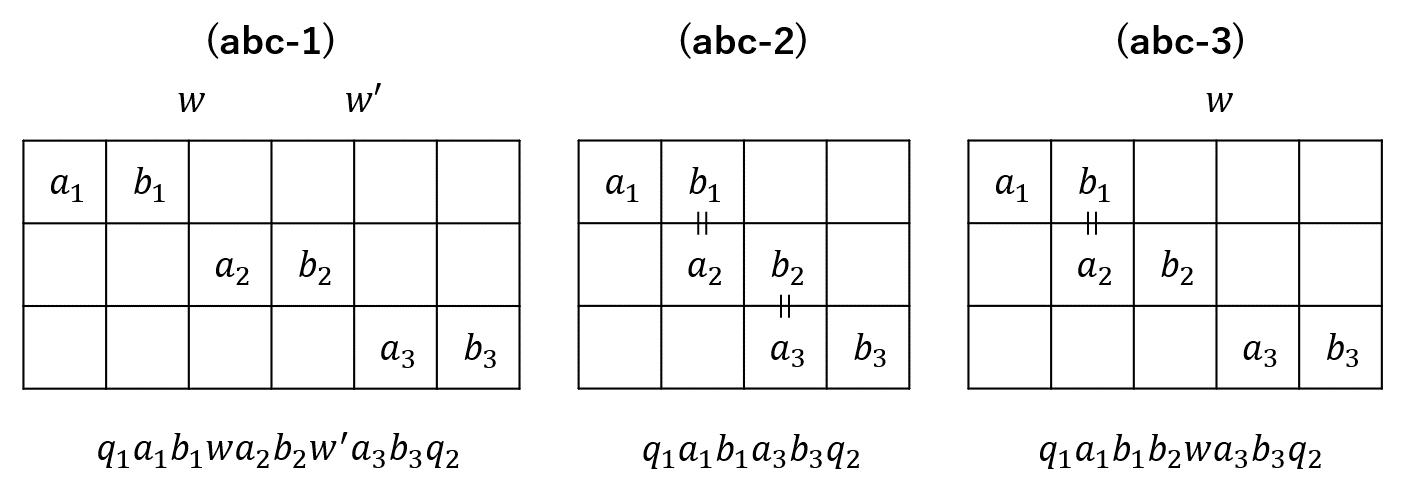
\includegraphics[width=\linewidth]{画像/abc組み合わせ.png}
\vspace{-1cm}
\caption{(abc)の場合分け}
\label{abc組み合わせ}
\end{figure}

図\ref{abc組み合わせ}のように,3つの記号列が重複する場合があるので,次の3つの場合に分けて証明する.
\[
\begin{tabular}{ll}
$\textbf{(abc-1)}$ $q=q_{1}a_{1}b_{1}wa_{2}b_{2}w^{\prime}a_{3}b_{3}q_{2}$,\\
$\textbf{(abc-2)}$ $q=q_{1}a_{1}b_{1}a_{3}b_{3}q_{2}$ ($b_{1}=a_{2}$かつ$a_{3}=b_{2}$),\\
$\textbf{(abc-3)}$ $q=q_{1}a_{1}b_{1}b_{2}wa_{3}b_{3}q_{2}$ ($b_{1}=a_{2}$).
\end{tabular}
\]

\textbf{(abc-1)} $q=q_{1}a_{1}b_{1}wa_{2}b_{2}w^{\prime}a_{3}b_{3}q_{2}$とする.これに対して,次の式が成り立っているものとする.
\begin{align*}
(1)~& p_{1} \preceq q_{1} & (\text{1'})~& p_{2} \preceq wa_{2}b_{2}w^{\prime}a_{3}b_{3}q_{2} \\
(2)~& p_{1} \preceq q_{1}a_{1}b_{1}w & (\text{2'})~& p_{2} \preceq w^{\prime}a_{3}b_{3}q_{2} \\
(3)~& p_{1} \preceq q_{1}a_{1}b_{1}wa_{2}b_{2}w^{\prime} & (\text{3'})~& p_{2} \preceq q_{2}
\end{align*}

$|w|=|w^{\prime}|$のとき,(2)と(3)より,$p_{1}$の接尾辞は$a_{1}b_{1}wa_{2}b_{2}w^{\prime}$かつ$a_{1}b_{1}w$であるので,$a_{1}b_{1}w=a_{2}b_{2}w^{\prime}$となる.よって,$a_{1}b_{1}=a_{2}b_{2}$となり,$a_{1} \ne a_{2}$かつ$b_{1} \ne b_{2}$であることに矛盾する.

$|w|+1=|w^{\prime}|$のとき,(1')と(2')より,$p_{2}$の接頭辞は$wa_{2}b_{2}w^{\prime}a_{3}b_{3}$かつ$w^{\prime}a_{3}b_{3}$である.
$w^{\prime}=ww_{1}$とおくと,$w^{\prime}a_{3}b_{3}=ww_{1}a_{3}b_{3}$となる.
したがって,$wa_{2}b_{2}=ww_{1}a_{3}$より$b_{2}=a_{3}$となる.
(2)と(3)より,$p_{1}$の接尾辞は$a_{1}b_{1}wa_{2}b_{2}w^{\prime}, a_{1}b_{1}w$である.$w^{\prime}=w_{2}w$とおくと,$a_{1}b_{1}wa_{2}b_{2}w^{\prime}=a_{1}b_{1}wa_{2}b_{2}w_{2}w$となる.
したがって,$b_{2}w_{2}w=a_{1}b_{1}w$より,$b_{2}=a_{1}$となる.
$b_{2}=a_{3}$より,$a_{3}=a_{1}$となり,$a_{3} \ne a_{1}$であることに矛盾する.

$|w|+1 < |w^{\prime}|$のとき,(2)と(3)より,$p_{1}$の接尾辞は$a_{1}b_{1}wa_{2}b_{2}w^{\prime}$かつ$a_{1}b_{1}w$である.
$w^{\prime}=w_{1}w$とおくと,$a_{1}b_{1}wa_{2}b_{2}w^{\prime}=a_{1}b_{1}wa_{2}b_{2}w_{1}w$となる.
$|w_{1}| \ge 2$であるため,$w_{1}$の接尾辞は$a_{2}b_{2}$となる.
($1'$)と($2'$)より,$p_{2}$の接頭辞は$wa_{2}b_{2}w^{\prime}a_{3}b_{3}$かつ$w^{\prime}a_{3}b_{3}$である.
$w^{\prime}=ww_{2}$とおくと,$w^{\prime}a_{3}b_{3}=ww_{2}a_{3}b_{3}$となり,$w^{\prime}=w_{1}w$とおくと,$wa_{2}b_{2}w^{\prime}a_{3}b_{3}=wa_{2}b_{2}w_{1}wa_{3}b_{3}$となる.
$|ww_{2}a_{3}b_{3}|=|wa_{2}b_{2}w_{1}|$より,$w_{1}$の接尾辞は$a_{3}b_{3}$となる.
よって,$w_{1}$の接尾辞は$a_{2}b_{2}=a_{3}b_{3}$となり,$a_{2} \ne a_{3}$かつ$b_{2} \ne b_{3}$であることに矛盾する.
\smallskip

\textbf{(abc-2)} $q=q_{1}a_{1}b_{1}a_{3}b_{3}q_{2}$ ($b_{1}=a_{2}$かつ$a_{3}=b_{2}$)とする.
これに対して,次の式が成り立っているものとする.
\begin{align*}
(1)~& p_{1} \preceq q_{1} & (\text{1'})~& p_{2} \preceq a_{3}b_{3}q_{2} \\
(2)~& p_{1} \preceq q_{1}a_{1} & (\text{2'})~& p_{2} \preceq b_{3}q_{2} \\
(3)~& p_{1} \preceq q_{1}a_{1}b_{1} & (\text{3'})~& p_{2} \preceq q_{2}
\end{align*}

(2)と(3)より,$p_{1}$の接尾辞は$a_{1}b_{1}$かつ$a_{1}$であり,$b_{1}=a_{1}$となる.$b_{1}=a_{2}$より,$a_{1}=a_{2}$であるため, $a_{1} \ne a_{2}$であることに矛盾する.
\smallskip

\textbf{(abc-3)} $q=q_{1}a_{1}b_{1}b_{2}wa_{3}b_{3}q_{2}$ ($b_{1}=a_{2}$)とする.これに対して,次の式が成り立っているものとする.
\begin{align*}
(1)~& p_{1} \preceq q_{1} & (\text{1'})~& p_{2} \preceq b_{2}wa_{3}b_{3}q_{2} \\
(2)~& p_{1} \preceq q_{1}a_{1} & (\text{2'})~& p_{2} \preceq wa_{3}b_{3}q_{2} \\
(3)~& p_{1} \preceq q_{1}a_{1}b_{1}b_{2}w & (\text{3'})~& p_{2} \preceq q_{2}
\end{align*}

$w=\varepsilon$のとき,(2)と(3)より,$p_{1}$の接尾辞は$a_{1}$かつ$a_{1}b_{1}b_{2}$であり,(1')と(2')より,$p_{2}$の接頭辞は$b_{2}a_{3}b_{3}$かつ$a_{3}b_{3}$である.
$b_{2}=a_{1}$と$b_{2}a_{3}=a_{3}b_{3}$より,$a_{1}=a_{3}$となり,$a_{1} \ne a_{3}$であることに矛盾する.

$|w| \ge 1$のとき,(2)と(3)より,$p_{1}$の接尾辞は$a_{1}$かつ$a_{1}b_{1}b_{2}w$である.
よって,$w$の最後の記号は$a_{1}$となる.
(1')と(2')より,$p_{2}$の接頭辞は$b_{2}wa_{3}b_{3}$かつ$wa_{3}b_{3}$となる.
よって,$w$の最後の記号は$a_{3}$となる.
したがって,$w$の最後の記号は$a_{1}=a_{3}$となり,$a_{1} \ne a_{3}$であることに矛盾する.
\smallskip

\textbf{(d)} $q$に$a_{1}b_{1}, a_{2}b_{2}, a_{3}y$が現れる場合,記号列$A,B,C$に対して,$\{ A, B, C \} = \{ a_{1}b_{1}, a_{2}b_{2}, a_{3}y \}$とおき,$q=q_{1}AwBw^{\prime}Cq_{2}$とする.
これに対して,次の式が成り立っているものとする.
\begin{align*}
(1)~& p_{1} \preceq q_{1} & (\text{1'})~& p_{2} \preceq wBw^{\prime}Cq_{2} \\
(2)~& p_{1} \preceq q_{1}Aw & (\text{2'})~& p_{2} \preceq w^{\prime}Cq_{2} \\
(3)~& p_{1} \preceq q_{1}AwBw^{\prime} & (\text{3'})~& p_{2} \preceq q_{2}
\end{align*}

$|w|=|w^{\prime}|$のとき,(2)と(3)より,$p_{1}$の接尾辞は$Aw$かつ$AwBw^{\prime}$である.
よって,$Aw=Bw^{\prime}$となり,$A \ne B$であることに矛盾する.

$|w| \ne |w^{\prime}|$とする.
$A=a_{3}y$とすると,$B=a_{1}b_{1}$,$C=a_{2}b_{2}$としてよいので,(2)は$p_{1} \preceq q_{1}a_{3}yw$となる.
したがって,正規パターン$p_{1}', p_{1}''$が存在して,$p_{1}=p_{1}'p_{1}''$,$p_{1}^{\prime} \preceq q_{1}a_{3}$かつ$p_{1}^{\prime\prime} \preceq yw$となる.
これらと(1')より,$p=p_{1}xp_{2}=p_{1}^{\prime}p_{1}^{\prime\prime}xp_{2}\preceq q_{1}a_{3}p_{1}^{\prime\prime}xwa_{1}b_{1}w^{\prime}a_{2}b_{2}q_{2}=q \{ y := p_{1}^{\prime\prime}x \}$となり,$p=q \theta$となる.
これは仮定に矛盾する.
$B=a_{3}y$とすると,$A=a_{1}b_{1}$,$C=a_{2}b_{2}$としてよいので,(3)は$p_{1} \preceq q_{1}a_{1}b_{1}wa_{3}yw^{\prime}$となり,(1')は$p_{2} \preceq wa_{3}yw^{\prime}a_{2}b_{2}q_{2}$である.$q_{1}^{\prime}=q_{1}a_{1}b_{1}$,$q_{2}^{\prime}=wa_{3}yw^{\prime}$,$q_{3}^{\prime}=a_{2}b_{2}q_{2}$とおくと, (3)~$p_{1} \preceq q_{1}^{\prime}q_{2}^{\prime}, (1')~p_{2} \preceq q_{2}^{\prime}q_{3}^{\prime}, q_{2}^{\prime}$は変数記号が含まれる.
補題\ref{補題9}より,$p \preceq q$となり,$p \{ x := xy \} \preceq q$である.
これは仮定に矛盾する.

以上より,$A$または$B$が$a_{3}y$の場合,仮定に矛盾するため,$C=a_{3}y$となる.

%\begin{figure}[H]
\begin{figure}
\centering
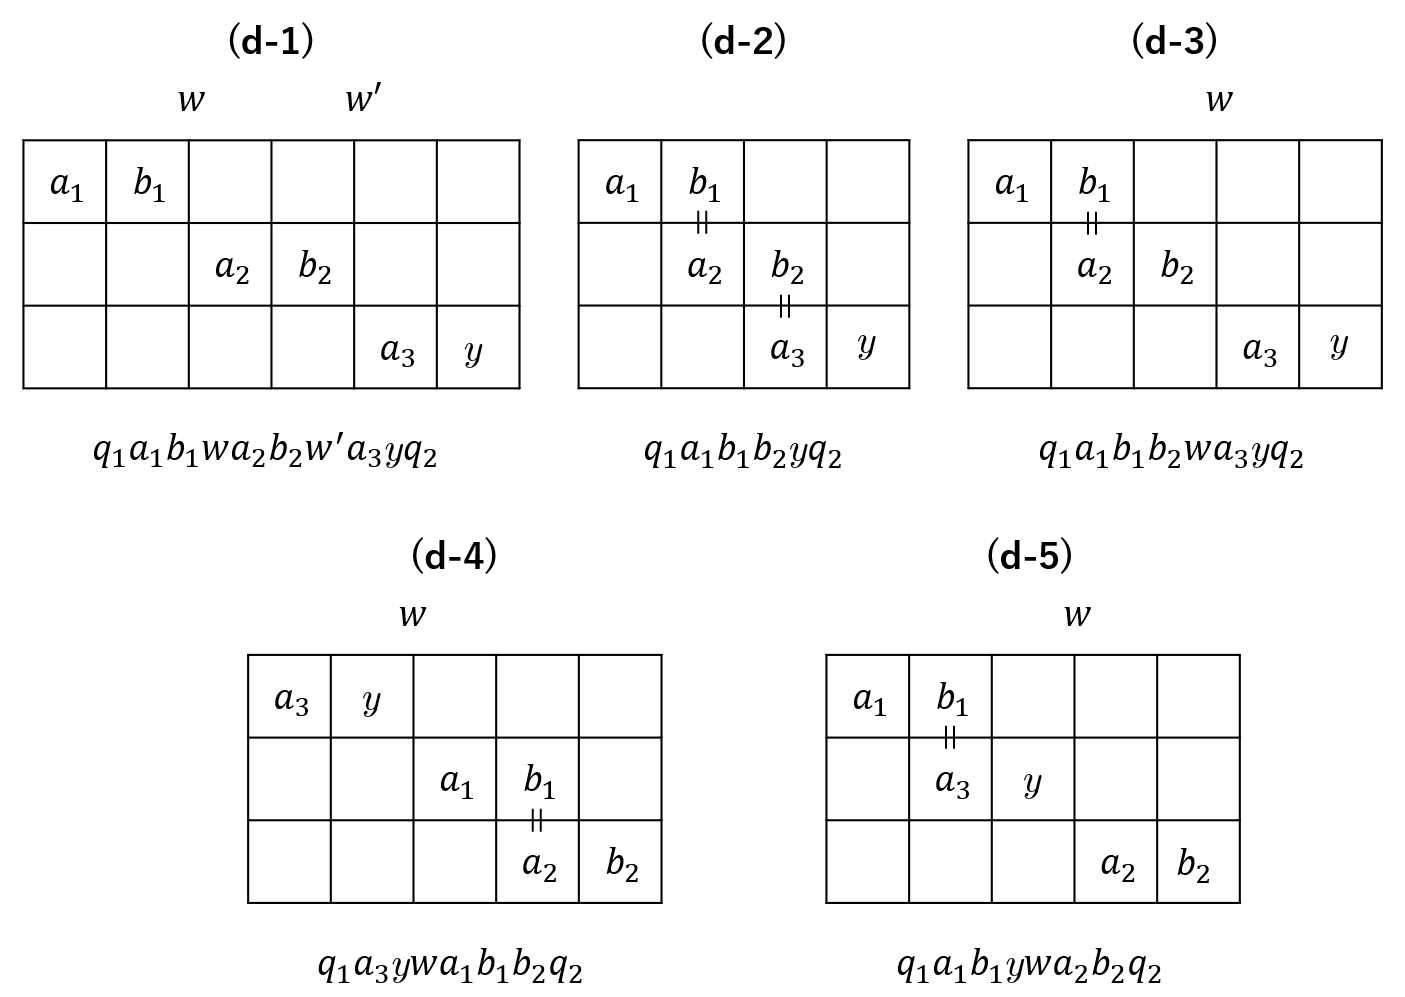
\includegraphics[width=\linewidth]{画像/d組み合わせ.png}
\vspace{-1cm}
\caption{(d)の場合分け}
\label{d組み合わせ}
\end{figure}

$C=a_{3}y$のとき,3つの記号列が重複する場合を考慮して,表\ref{d組み合わせ}のように,5つの場合に分けて証明する.
\[
\begin{tabular}{ll}
$\textbf{(d-1)}$ $q=q_{1}a_{1}b_{1}wa_{2}b_{2}w^{\prime}a_{3}yq_{2}$,\\
$\textbf{(d-2)}$ $q=q_{1}a_{1}b_{1}b_{2}yq_{2}$ ($a_{2}=b_{1}$かつ$a_{3}=b_{2}$),\\
$\textbf{(d-3)}$ $q=q_{1}a_{1}b_{1}b_{2}wa_{3}yq_{2}$ ($b_{1}=a_{2}$),\\
$\textbf{(d-4)}$ $q=q_{1}a_{3}ywa_{1}b_{1}b_{2}q_{2}$ ($b_{1}=a_{2}$),\\
$\textbf{(d-5)}$ $q=q_{1}a_{1}b_{1}ywa_{2}b_{2}q_{2}$ ($b_{1}=a_{3}$).
\end{tabular}
\]

\textbf{(d-1)} $q=q_{1}a_{1}b_{1}wa_{2}b_{2}w^{\prime}a_{3}yq_{2}$とする.これに対して,次の式が成り立っているものとする.
\begin{align*}
(1)~& p_{1} \preceq q_{1} & (\text{1'})~& p_{2} \preceq wa_{2}b_{2}w^{\prime}a_{3}yq_{2} \\
(2)~& p_{1} \preceq q_{1}a_{1}b_{1}w & (\text{2'})~& p_{2} \preceq w^{\prime}a_{3}yq_{2} \\
(3)~& p_{1} \preceq q_{1}a_{1}b_{1}wa_{2}b_{2}w^{\prime} & (\text{3'})~& p_{2} \preceq q_{2}
\end{align*}

$|w|+1=|w^{\prime}|$のとき,(2)と(3)より,$p_{1}$の接尾辞は$a_{1}b_{1}wa_{2}b_{2}w^{\prime}$かつ$a_{1}b_{1}w$である.
$w^{\prime}=w_{1}w$とおくと,$a_{1}b_{1}wa_{2}b_{2}w^{\prime}=a_{1}b_{1}wa_{2}b_{2}w_{1}w$と表すことができる.
$b_{2}w_{1}w=a_{1}b_{1}w$より,$b_{2}=a_{1}$となる.
(1')と(2')より,$p_{2}$の接頭辞は$wa_{2}b_{2}w^{\prime}a_{3}$かつ$w^{\prime}a_{3}$である.
$w^{\prime}=ww_{2}$とおくと, $w^{\prime}a_{3}=ww_{2}a_{3}$と表すことができる.$wa_{2}b_{2}=ww_{2}a_{3}$より,$b_{2}=a_{3}$となる.
よって,$b_{2}=a_{1}$より,$a_{1}=a_{3}$となり,$a_{1} \ne a_{3}$であることに矛盾する.

$|w|+1 < |w^{\prime}|$のとき,(2)と(3)より,$p_{1}$の接尾辞は$a_{1}b_{1}wa_{2}b_{2}w^{\prime}$かつ$a_{1}b_{1}w$である.
$w^{\prime}=w_{1}w$とおくと,$a_{1}b_{1}wa_{2}b_{2}w^{\prime}=a_{1}b_{1}wa_{2}b_{2}w_{1}w$と表すことができる.
よって,$w_{1}$の接尾辞は$a_{1}b_{1}$となる.
(1')と(2')より,$p_{2}$の接頭辞は$wa_{2}b_{2}w^{\prime}a_{3}$かつ$w^{\prime}a_{3}$である.
$w^{\prime}=w_{1}w$とおくと,$wa_{2}b_{2}w^{\prime}a_{3}=wa_{2}b_{2}w_{1}wa_{3}$となる.
さらに,$w^{\prime}=ww_{2}$とおくと,$w^{\prime}a_{3}=ww_{2}a_{3}$と表すことができる.$|a_{2}b_{2}w_{1}|=|w_{2}a_{3}|+1$より,$w_{1}$の最後から2つ目の記号は$a_{3}$となる.よって,$w_{1}$の接尾辞は$a_{1}b_{1}$であり,$a_{1}=a_{3}$となる.
これは,$a_{1} \ne a_{3}$であることに矛盾する.

$|w^{\prime}|+1=|w|$のとき,(1')と(2')より,$p_{2}$の接頭辞は$wa_{2}b_{2}w^{\prime}a_{3}$かつ$w^{\prime}a_{3}$である.
$w=w^{\prime}w_{1}$とおくと,$wa_{2}b_{2}w^{\prime}a_{3}=w^{\prime}w_{1}a_{2}b_{2}w^{\prime}a_{3}$と表すことができる.
$w^{\prime}w_{1}=w^{\prime}a_{3}$より,$w_{1}=a_{3}$となる.(2)と(3)より,$p_{1}$の接尾辞は$a_{1}b_{1}wa_{2}b_{2}w^{\prime}$かつ$a_{1}b_{1}w$である.
$w=w^{\prime}w_{1}$とおくと,$a_{1}b_{1}wa_{2}b_{2}w^{\prime}=a_{1}b_{1}w^{\prime}w_{1}a_{2}b_{2}w^{\prime}$となる.
さらに,$w=w_{2}w^{\prime}$とおくと,$a_{1}b_{1}w=a_{1}b_{1}w_{2}w^{\prime}$と表すことができる.
$|w_{1}a_{2}b_{2}w^{\prime}|=|a_{1}b_{1}w_{2}w^{\prime}|$より,$w_{1}=a_{1}$となる.よって,$w_{1}=a_{3}$より,$a_{1}=a_{3}$となり,$a_{1} \ne a_{3}$であることに矛盾する.

$|w| > |w^{\prime}|+1$のとき,(1')と(2')より,$p_{2}$の接頭辞は$wa_{2}b_{2}w^{\prime}a_{3}$かつ$w^{\prime}a_{3}$である.
$w=w^{\prime}w_{1}$とおくと,$wa_{2}b_{2}w^{\prime}a_{3}=w^{\prime}w_{1}a_{2}b_{2}w^{\prime}a_{3}$と表すことができる.
このとき,$w_{1}$の最初の記号は$a_{3}$となる.(2)と(3)より,$p_{1}$の接尾辞は$a_{1}b_{1}wa_{2}b_{2}w^{\prime}$かつ$a_{1}b_{1}w$である.
$w=w^{\prime}w_{1}$とおくと,$a_{1}b_{1}wa_{2}b_{2}w^{\prime}=a_{1}b_{1}w^{\prime}w_{1}a_{2}b_{2}w^{\prime}$となる.
さらに,$w=w_{2}w^{\prime}$とおくと,$a_{1}b_{1}w=a_{1}b_{1}w_{2}w^{\prime}$と表すことができる.
$|w_{1}a_{2}b_{2}|=|a_{1}b_{1}w_{2}|$より,$w_{1}$の接頭辞は$a_{1}b_{1}$となる.
よって,$w_{1}$の接頭辞は$a_{3}$であり,$a_{1}b_{1}$である.
すなわち,$a_{3}=a_{1}$となる.
これは,$a_{3} \ne a_{1}$であることに矛盾する.
\smallskip

\textbf{(d-2)} $q=q_{1}a_{1}b_{1}b_{2}yq_{2}$ ($a_{2}=b_{1}$かつ$a_{3}=b_{2}$)とする.
これに対して,次の式が成り立っているものとする.
\begin{align*}
(1)~& p_{1} \preceq q_{1} & (\text{1'})~& p_{2} \preceq b_{2}yq_{2} \\
(2)~& p_{1} \preceq q_{1}a_{1} & (\text{2'})~& p_{2} \preceq yq_{2} \\
(3)~& p_{1} \preceq q_{1}a_{1}b_{1} & (\text{3'})~& p_{2} \preceq q_{2}
\end{align*}

(2)と(3)より,$p_{1}$の接尾辞は$a_{1}b_{1}$かつ$a_{1}$である.
よって,$b_{1}=a_{1}$となる.$a_{2}=b_{1}$より,$a_{1}=a_{2}$となり,$a_{1} \ne a_{2}$であることに矛盾する.
\smallskip

\textbf{(d-3)} $q=q_{1}a_{1}b_{1}b_{2}wa_{3}yq_{2}$ ($b_{1}=a_{2}$)とする.これに対して,次の式が成り立っているものとする.
\begin{align*}
(1)~& p_{1} \preceq q_{1} & (\text{1'})~& p_{2} \preceq b_{2}wa_{3}yq_{2} \\
(2)~& p_{1} \preceq q_{1}a_{1} & (\text{2'})~& p_{2} \preceq wa_{3}yq_{2} \\
(3)~& p_{1} \preceq q_{1}a_{1}b_{1}b_{2}w & (\text{3'})~& p_{2} \preceq q_{2}
\end{align*}

$w=\varepsilon$のとき,(2)と(3)より,$p_{1}$の接尾辞は$a_{1}$かつ$a_{1}b_{1}b_{2}$である.
よって,$a_{1}=b_{2}$となる.
(1')と(2')より,$p_{2}$の接頭辞は$b_{2}a_{3}$かつ$a_{3}$である.
よって,$b_{2}=a_{3}$となる.
したがって,$a_{1}=b_{2}$より,$a_{1}=a_{3}$となり,$a_{1} \ne a_{3}$であることに矛盾する.

$|w| \ge 1$のとき,(2)と(3)より,$p_{1}$の接尾辞は$a_{1}$かつ$a_{1}b_{1}b_{2}w$である.
よって,$w$の最後の記号は$a_{1}$となる.
(1')と(2')より,$p_{2}$の接頭辞は$b_{2}wa_{3}$かつ$wa_{3}$である.
よって,$w$の最後の記号は$a_{3}$となる.
したがって,$w$の最後の記号は$a_{1}=a_{3}$となり,$a_{1} \ne a_{3}$であることに矛盾する.
\smallskip

\textbf{(d-4)} $q=q_{1}a_{3}ywa_{1}b_{1}b_{2}q_{2}$ ($b_{1}=a_{2}$)とする.これに対して,次の式が成り立っているものとする.
\begin{align*}
(1)~& p_{1} \preceq q_{1} & (\text{1'})~& p_{2} \preceq wa_{1}b_{1}b_{2}q_{2} \\
(2)~& p_{1} \preceq q_{1}a_{3}yw & (\text{2'})~& p_{2} \preceq b_{2}q_{2} \\
(3)~& p_{1} \preceq q_{1}a_{3}ywa_{1} & (\text{3'})~& p_{2} \preceq q_{2}
\end{align*}

(3)より,正規パターン$p_{1}^{\prime}$と$p_{1}^{\prime\prime}$が存在して,$p_{1}=p_{1}^{\prime}p_{1}^{\prime\prime}$,$p_{1}^{\prime} \preceq q_{1}a_{3}$かつ$p_{1}^{\prime\prime} \preceq ywa_{1}$が成り立つ.
これらより,$p=p_{1}xp_{2}=p_{1}^{\prime}p_{1}^{\prime\prime}xp_{2}\preceq q_{1}a_{3}p_{1}^{\prime\prime}xwa_{1}b_{1}b_{2}q_{2}=q \{ y := p_{1}^{\prime\prime}x \}$となるので,$p \preceq q$となり,$p \{ x := xy \} \preceq q$である.これは仮定に矛盾する.
\smallskip

\textbf{(d-5)} $q=q_{1}a_{1}b_{1}ywa_{2}b_{2}q_{2}$ ($b_{1}=a_{3}$)とする.これに対して,次の式が成り立っているものとする.
\begin{align*}
(1)~& p_{1} \preceq q_{1} & (\text{1'})~& p_{2} \preceq ywa_{2}b_{2}q_{2} \\
(2)~& p_{1} \preceq q_{1}a_{1} & (\text{2'})~& p_{2} \preceq wa_{2}b_{2}q_{2} \\
(3)~& p_{1} \preceq q_{1}a_{1}b_{1}yw & (\text{3'})~& p_{2} \preceq q_{2}
\end{align*}

$q_{1}^{\prime}=q_{1}a_{1}b_{1}$,$q_{2}^{\prime}=yw$,$q_{3}^{\prime}=a_{2}b_{2}q_{2}$とおくと,(3)から,$p_{1} \preceq q_{1}^{\prime}q_{2}^{\prime}$,(1')から$p_{2} \preceq q_{2}^{\prime}q_{3}^{\prime}$が得られ,さらに$q_{2}^{\prime}$は変数記号が含まれるので,補題\ref{補題9}より,$p \preceq q$となり,$p \{ x := xy \} \preceq q$である.
これは仮定に矛盾する.
%\hspace{\fill}\rm{(Q.E.D)}

\end{proof}

\begin{lem}\label{追加部分}
$\sharp \Sigma \ge 3$とし,$p, q$を正規パターンとする.
正規パターンの有限集合$D= \{ ya, bc, dy \}$ $(b \not = a,dかつc \not = a,d)$で表されるとき,任意の$r \in D$に対して$p \{ x := r \} \preceq q$ならば,$p \{ x := xy \} \preceq q$である.
\end{lem}
\begin{proof}
$p$に変数記号が現れない場合は自明である.
したがって,$p=p_{1}xp_{2}$ ($p_{1}, p_{2}$は正規パターン,$x$は変数記号)とおく.$p \{ x := xy \} \not \preceq q$と仮定して,矛盾を導く.

記号列$A,B,C$に対して,$\{ A,B,C \} = \{ y_{1}a,bc,dy_{2} \}$とおき,$q=q_{1}AwBw^{\prime}Cq_{2}$とする.
これに対して,次の式が成り立っているものとする.
\begin{align*}
(1)~& p_{1} \preceq q_{1} & (\text{1'})~& p_{2} \preceq wBw^{\prime}Cq_{2} \\
(2)~& p_{1} \preceq q_{1}Aw & (\text{2'})~& p_{2} \preceq w^{\prime}Cq_{2} \\
(3)~& p_{1} \preceq q_{1}AwBw^{\prime} & (\text{3'})~& p_{2} \preceq q_{2}
\end{align*}

$q^{\prime}_{1}=q_{1}A,q^{\prime}_{2}=wBw^{\prime},q^{\prime}_{3}=Cq_{2}$とおくと,(3)と(1')より,$p_{1} \preceq q^{\prime}_{1}q^{\prime}_{2},p_{2} \preceq q^{\prime}_{2}q^{\prime}_{3}$となる.
補題\ref{補題9}より,$q^{\prime}_{2}$に変数記号が含まれるとき,$p \preceq q$となる.
よって,$B=y_{1}a$または,$B=dy_{2}$である場合,仮定に矛盾する.
したがって,$B=bc$である場合のみを考える.

$A=dy_{2}$とすると,(2)は$p_{1} \preceq q_{1}dy_{2}w$となる.
$p_{1}=p^{\prime}_{1}p^{\prime\prime}_{1}, p^{\prime}_{1} \preceq q_{1}d$かつ$p^{\prime\prime}_{1} \preceq y_{2}w$とおくと,(1')より,$p=p_{1}xp_{2}=p^{\prime}_{1}p^{\prime\prime}_{1}xp_{2} \preceq q_{1}dp^{\prime\prime}_{1}xwbcw^{\prime}y_{1}aq_{2}=q \{ x:=p^{\prime\prime}_{1}x \}$となり,$p=q\theta$となる.
これは仮定に矛盾する.
したがって,$A=y_{1}a,B=bc,C=dy_{2}$である場合のみ考えればよい.

$q=q_{1}y_{1}awbcw^{\prime}dy_{2}q_{2}~(b \not = a,d$かつ$c \not = a,d)$とする.
これに対して,次の式が成り立っているものとする.
\begin{align*}
(1)~& p_{1} \preceq q_{1} & (\text{1'})~& p_{2} \preceq wbcw^{\prime}dy_{2}q_{2} \\
(2)~& p_{1} \preceq q_{1}y_{1}aw & (\text{2'})~& p_{2} \preceq w^{\prime}dy_{2}q_{2} \\
(3)~& p_{1} \preceq q_{1}y_{1}awbcw^{\prime} & (\text{3'})~& p_{2} \preceq q_{2}
\end{align*}

$|w|=|w^{\prime}|$のとき,(2)と(3)より,$p_{1}$の接尾辞は$awbcw^{\prime}$かつ$aw$であるので,$cw^{\prime}=aw$となる.
これは,$c=a$となり,$c \not = a$であることに矛盾する.

$|w| = |w^{\prime}|+1$のとき,(2)と(3)より,$p_{1}$の接尾辞は$awbcw^{\prime}$かつ$aw$である.
$w=w_{1}w^{\prime}$とおくと,$aw=aw_{1}w^{\prime}$となる.
したがって,$bcw^{\prime}=aw_{1}w^{\prime}$より,$b = a$となる.
これは$b \not = a$であることに矛盾する.

$|w| = |w^{\prime}|+2$のとき,(2)と(3)より,$p_{1}$の接尾辞は$awbcw^{\prime}$かつ$aw$であり,(1')と(2')より,$p_{2}$の接頭辞は$wbcw^{\prime}d$かつ$w^{\prime}d$である.

%\begin{figure}[H]
\begin{figure}  
\centering
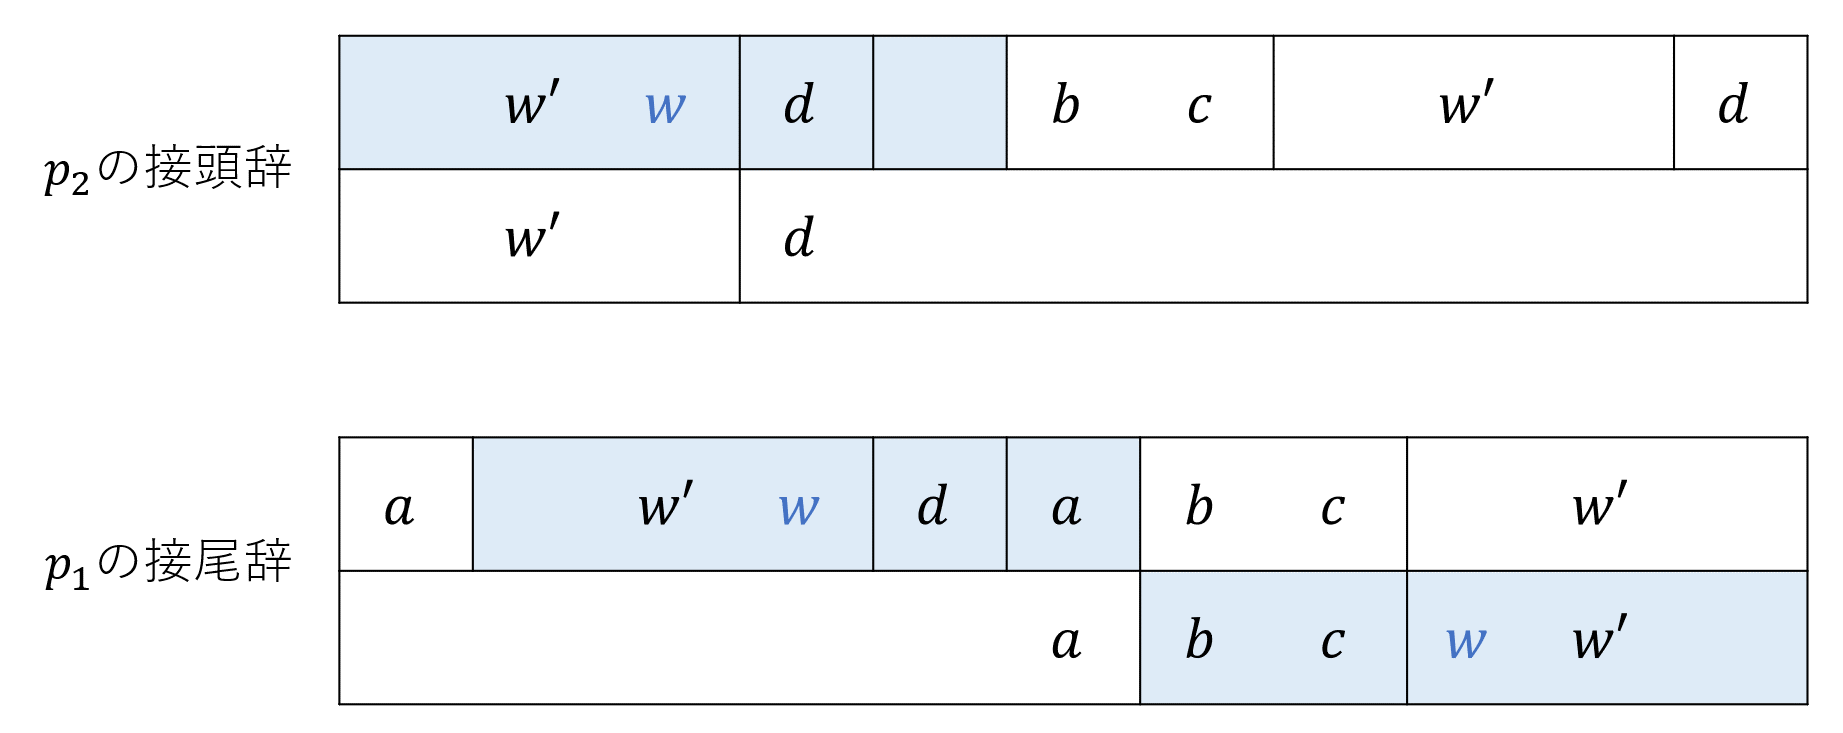
\includegraphics[width=\linewidth]{画像/追加部分1.png}
\vspace{-1cm}
\caption{$|w| = |w^{\prime}|+2$における\,$p_{1}$\,の接尾辞,$p_{2}$\,の接頭辞の関係}
\label{追加部分1}
\vspace*{-.2cm}
\end{figure}

図\ref{追加部分1}のように,$w=w^{\prime}da,w=bcw^{\prime}$となる.
よって,$w^{\prime}da=bcw^{\prime}$となる.

\begin{cl}\label{主張1}
$w^{\prime}$を定数記号列,a,b,c,dを定数記号とする.
このとき,$w^{\prime}da \not =bcw^{\prime}$ $(b \not = a,d$かつ$c \not = a,d)$となる.
\end{cl}

\noindent\textbf{主張\ref{主張1}の証明.}
$w^{\prime}da=bcw^{\prime}$と仮定する.
$|w^{\prime}| \ge 4$のとき,$w^{\prime}=bcw_{1}da$ $(w_{1}は定数記号列)$とおける.
$w^{\prime}da=bcw_{1}dada, bcw^{\prime}=bcbcw_{1}da$であるので,$bcw_{1}dada=bcbcw_{1}da$となる.
$w^{\prime}$と同様に$w_{1}$を考えると,$w_{1}=bcw_{2}da$ $(w_{2}は定数記号列)$とおける.
$w_{2}$以降も同様に定義できる.
ここで,定数記号列の長さを考えていくと,$|w_{1}|=|w^{\prime}|-4, |w_{2}|=|w_{1}|-4$のように,$|w_{i+1}|$は$|w_{i}|$より長さ4ずつ短くなっていく.
そのため,定数記号列を繰り返し定義していくと,最終的に定義できる$w_{n}$は長さ0,1,2,3のいずれかとなる.

%\begin{figure}[H]
\begin{figure}  
\centering
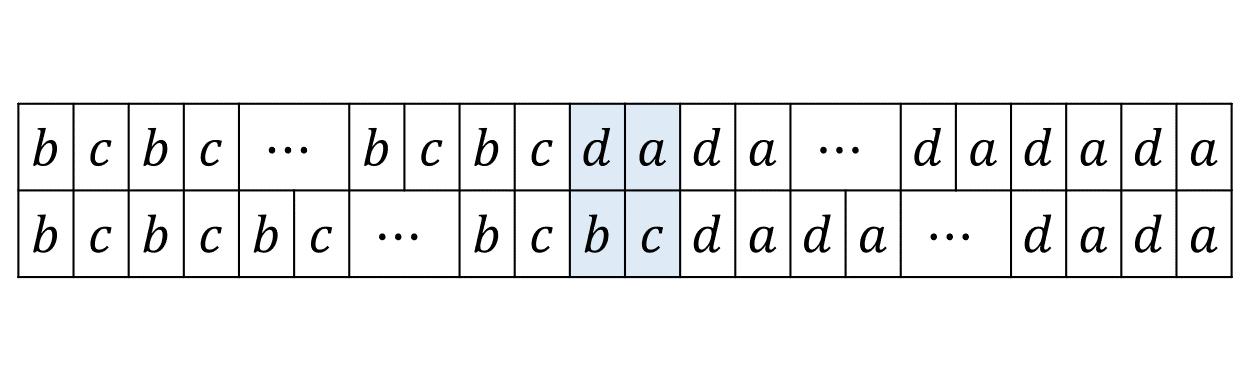
\includegraphics[width=\linewidth]{画像/追加部分2.png}
\vspace{-1.5cm}
\caption{$|w_{n}| = 0$における定数記号列}
\label{追加部分2}
\vspace*{-.2cm}
\end{figure}


$|w_{n}|=0$のとき,図\ref{追加部分2}のように,$da=bc$となる.
これは,$b \not = d$であることに矛盾する.

%\begin{figure}[H]
\begin{figure}
\centering
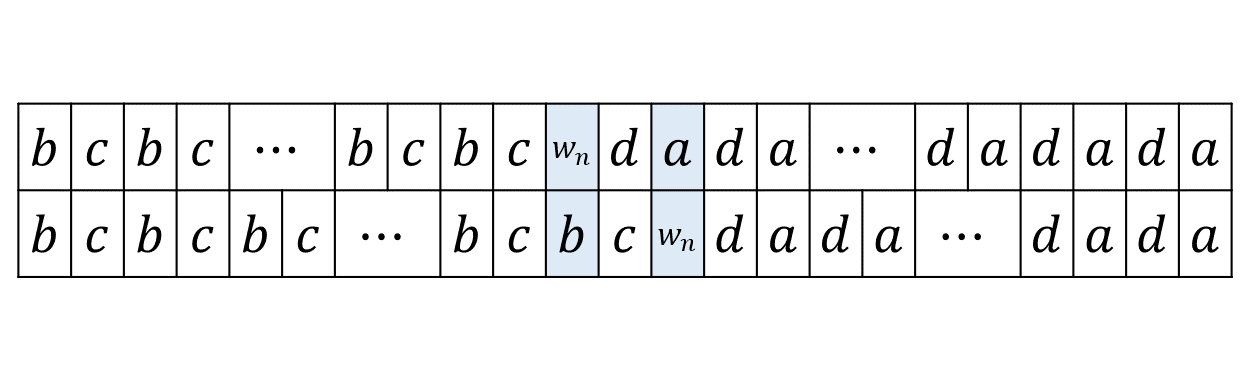
\includegraphics[width=\linewidth]{画像/追加部分3.png}
\vspace{-1.5cm}
\caption{$|w_{n}| = 1$における定数記号列}
\label{追加部分3}
\vspace*{-.2cm}
\end{figure}


$|w_{n}|=1$のとき,図\ref{追加部分3}のように,$w_{n}=a=b$となる.
これは,$b \not = a$であることに矛盾する.

%\begin{figure}[H]
\begin{figure}  
\centering
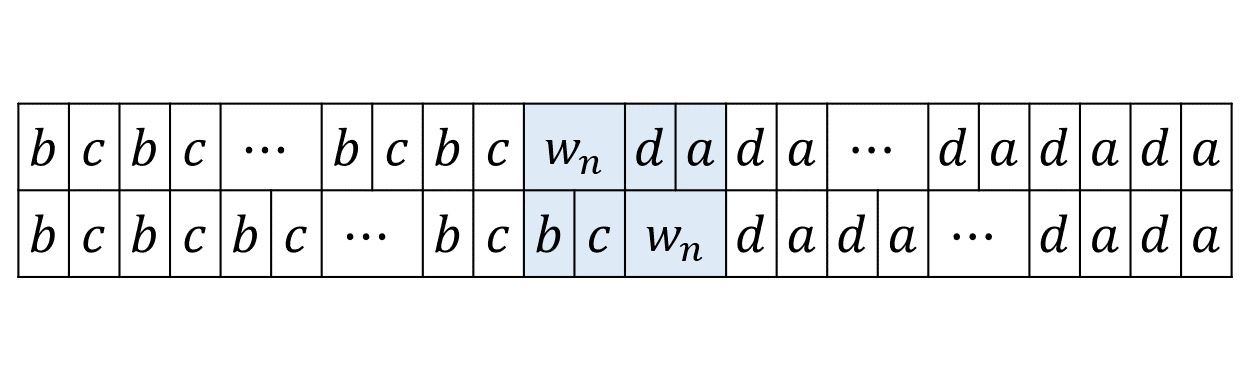
\includegraphics[width=\linewidth]{画像/追加部分4.png}
\vspace{-1.5cm}
\caption{$|w_{n}| = 2$における定数記号列}
\label{追加部分4}
\vspace*{-.2cm}
\end{figure}

$|w_{n}|=2$のとき,図\ref{追加部分4}のように,$w_{n}=bc=da$となる.
これは,$b \not = d$であることに矛盾する.

%\begin{figure}[H]
\begin{figure}  
\centering
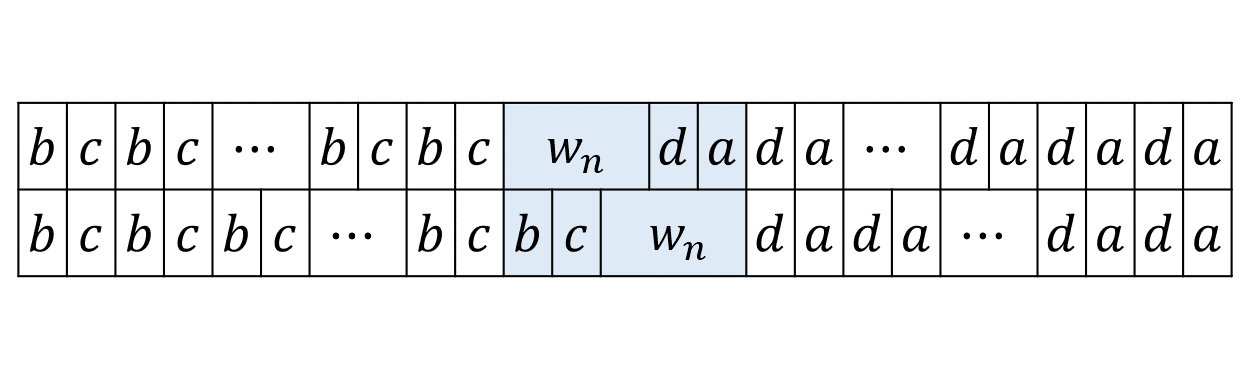
\includegraphics[width=\linewidth]{画像/追加部分5.png}
\vspace{-1.5cm}
\caption{$|w_{n}| = 3$における定数記号列}
\label{追加部分5}
\end{figure}

$|w_{n}|=3$のとき,$w_{n}=w_{n_{1}}w_{n_{2}}w_{n_{3}} (w_{n_{i}}はw_{n}におけるi番目の定数記号)$と表すと,図\ref{追加部分5}のように,$bcw_{n_{3}}=w_{n_{1}}da$となる.
よって,$c=d$となる.
これは,$c \not = d$であることに矛盾する.

以上より,$|w_{n}|=0,1,2,3$のとき,すべての場合において,仮定に矛盾するため,$|w^{\prime}| \ge 4$である場合,$w^{\prime}da \not = bcw^{\prime}$となる.

$|w^{\prime}| \le 3$のとき,$|w_{n}|=0,1,2,3$を$|w^{\prime}|$と置き換えて考えることができるため,すべての場合において仮定に矛盾する.
よって,$w^{\prime}da \not = bcw^{\prime}$となる.

\hspace{\fill}\rm{(主張\ref{主張1}のQ.E.D)}

よって,$w^{\prime}da=bcw^{\prime}$は,主張\ref{主張1}に矛盾する.

%\begin{figure}[H]
\begin{figure}  
\centering
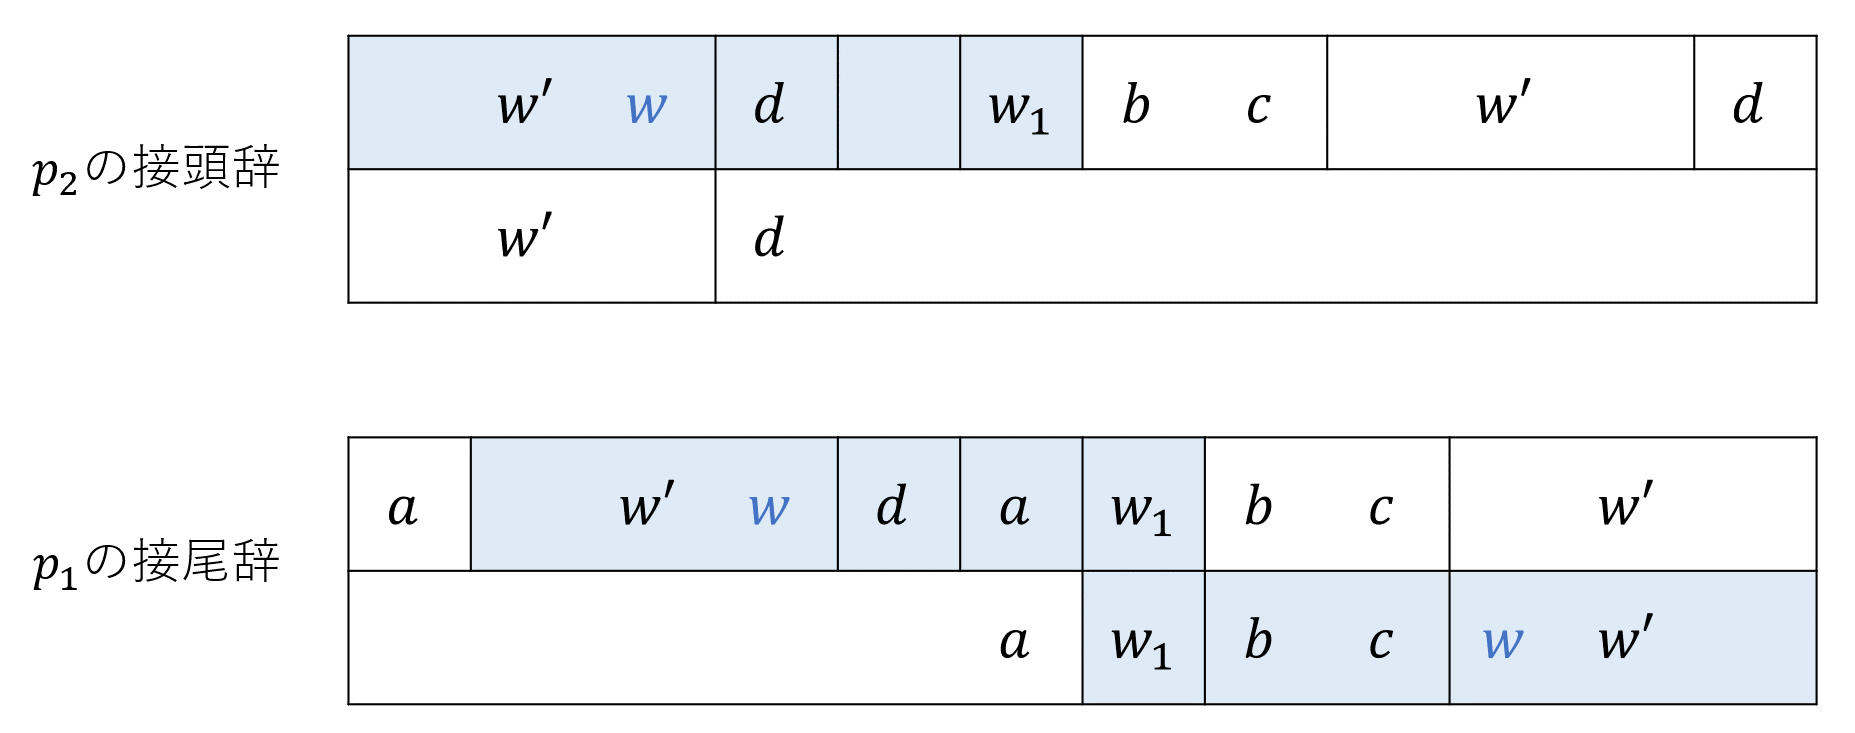
\includegraphics[width=\linewidth]{画像/追加部分6.png}
\vspace{-1cm}
\caption{$|w| \ge |w^{\prime}|+3$における$p_{1}$の接尾辞,$p_{2}$の接頭辞の関係}
\label{追加部分6}
\end{figure}

$|w| \ge |w^{\prime}|+3$のとき,図\ref{追加部分6}のように,$w=w^{\prime}daw_{1}=w_{1}bcw^{\prime}$ $(w_{1}は定数記号列)$となる.
よって,$w^{\prime}daw_{1}=w_{1}bcw^{\prime}$となる.

\begin{cl}\label{主張2}
$w, w_{1}$を定数記号列,a,b,c,dを定数記号とする.
このとき,$wdaw_{1} \not =w_{1}bcw$ $(b \not = a,d$かつ$c \not = a,d)$となる.
\end{cl}

\noindent\textbf{主張\ref{主張2}の証明.}
$wdaw_{1}=w_{1}bcw$と仮定する.
$w$と$w_{1}$の関係を以下のように場合分けして,考えていく.
\[
\begin{tabular}{ll}
$\textbf{(a)}$ $|w_{1}| \le |w| \le |w_{1}|+2$,\\
$\textbf{(b)}$ $2|w_{1}| \le |w| \le 2|w_{1}|+4$,\\
$\textbf{(c)}$ $|w_{1}|=0$,\\
$\textbf{(d)}$ $|w_{1}|+3 \le |w| \le 2|w_{1}|-1$,\\
$\textbf{(e)}$ $|w| \ge 2|w_{1}|+5$. 
\end{tabular}
\]

\noindent$\textbf{(a)}$ $|w_{1}| \le |w| \le |w_{1}|+2$である場合から考える.

%\begin{figure}[H]
\begin{figure} 
\centering
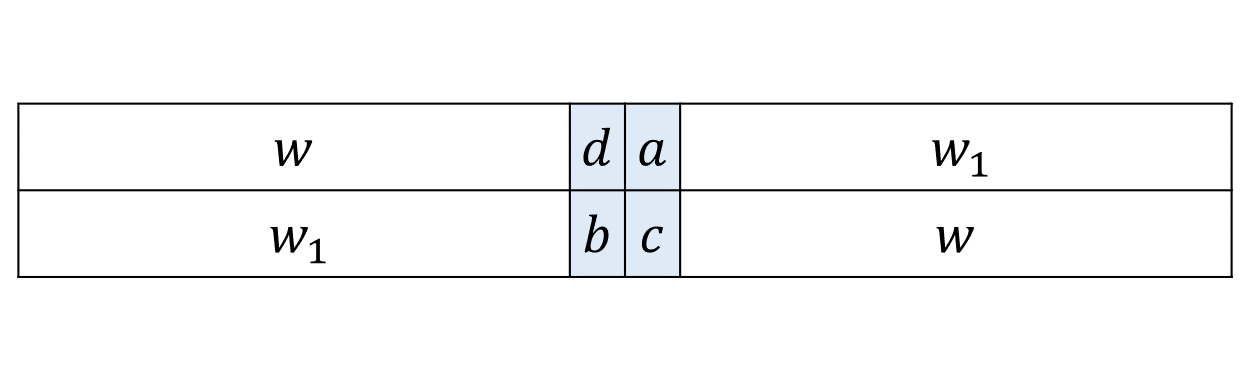
\includegraphics[width=\linewidth]{画像/追加部分7.png}
\vspace{-1.5cm}
\caption{$|w| = |w_{1}|$における定数記号列}
\label{追加部分7}
\vspace*{-.4cm}
\end{figure}

$|w|=|w_{1}|$のとき,図\ref{追加部分7}のように,$bc=da$となる.
これは,$b \not = d$であることに矛盾する.

%\begin{figure}[H]
\begin{figure}  
\centering
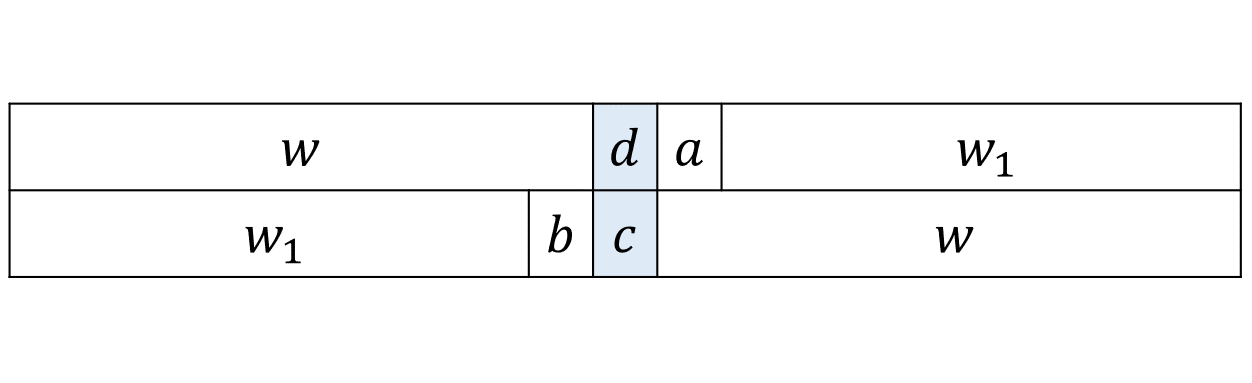
\includegraphics[width=\linewidth]{画像/追加部分8.png}
\vspace{-1.5cm}
\caption{$|w| = |w_{1}|+1$における定数記号列}
\label{追加部分8}
\vspace*{-.4cm}
\end{figure}

$|w|=|w_{1}|+1$のとき,図\ref{追加部分8}のように,$c=d$となる.
これは,$c \not = d$であることに矛盾する.

%\begin{figure}[H]
%\begin{figure}  
%\centering
%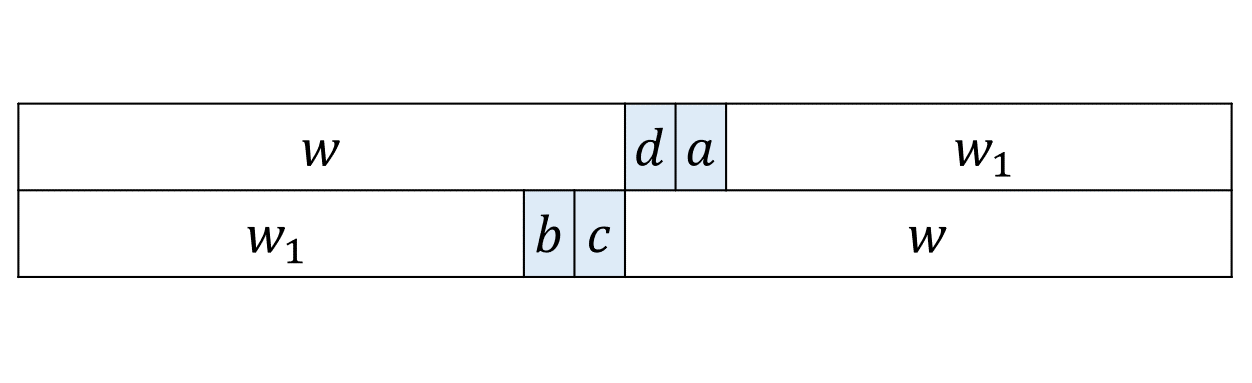
\includegraphics[width=\linewidth]{画像/追加部分9.png}
%\vspace{-1.5cm}
%\caption{$|w| = |w_{1}|+2$における定数記号列}
%\label{追加部分9}
%\vspace*{-.4cm}
%\end{figure}

$|w|=|w_{1}|+2$のとき,図\ref{追加部分9}のように,$w=w_{1}bc=daw_{1}$となる.
これは,主張\ref{主張1}に矛盾する.

\noindent$\textbf{(b)}$ $2|w_{1}| \le |w| \le 2|w_{1}|+4$である場合,

$|w|=2|w_{1}|$のとき,図\ref{追加部分14}のように,$w_{1}da=bcw_{1}$となる.
これは,主張\ref{主張1}に矛盾する.

$|w|=2|w_{1}|+1$のとき,図\ref{追加部分13}のように,$b=a$となる.
これは,$b \not = a$であることに矛盾する.

$|w|=2|w_{1}|+2$のとき,図\ref{追加部分12}のように,$bc=da$となる.
これは,$b \not = d$であることに矛盾する.

$|w|=2|w_{1}|+3$のとき,図\ref{追加部分11}のように,$c=d$となる.
これは,$c \not = d$であることに矛盾する.

%\begin{figure}[H]
\begin{figure}  
\centering
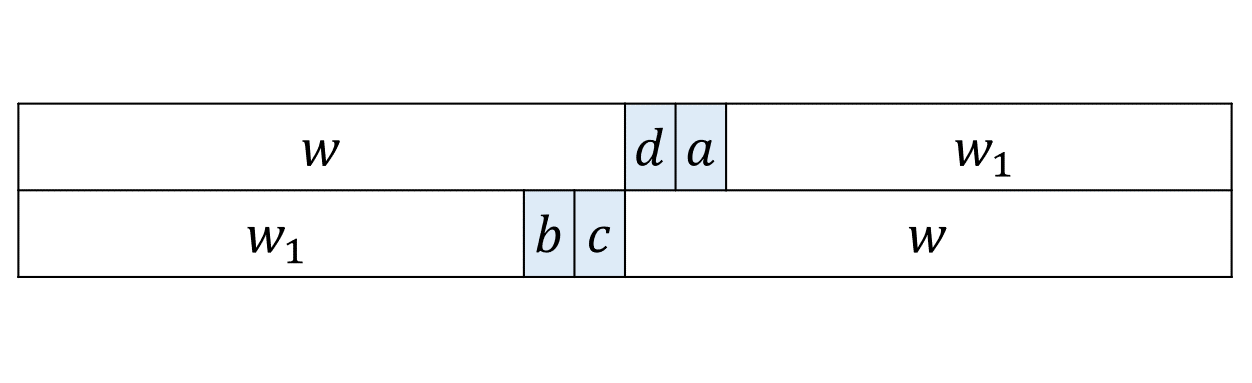
\includegraphics[width=\linewidth]{画像/追加部分9.png}
\vspace{-1.0cm}
\caption{$|w| = |w_{1}|+2$における定数記号列}
\label{追加部分9}
\vspace*{.5cm}

\centering
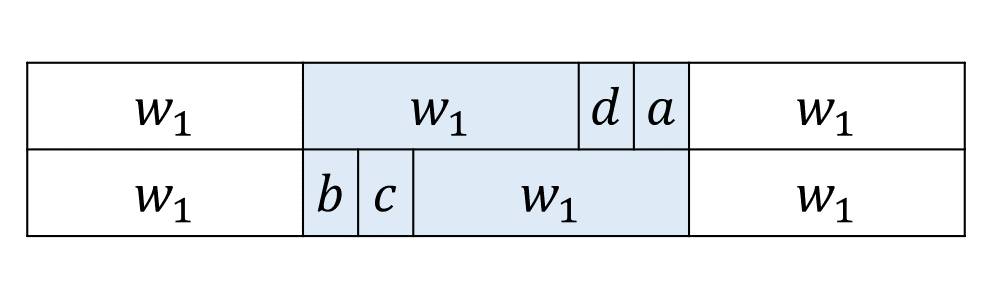
\includegraphics[scale=.4]{画像/追加部分14.png}
\vspace{-.4cm}
\caption{$|w| = 2|w_{1}|$における定数記号列}
\label{追加部分14}
\vspace*{.5cm}
%\vspace*{-.2cm}
%\end{figure}
%
%\begin{figure}[H]
%\begin{figure}  
\centering
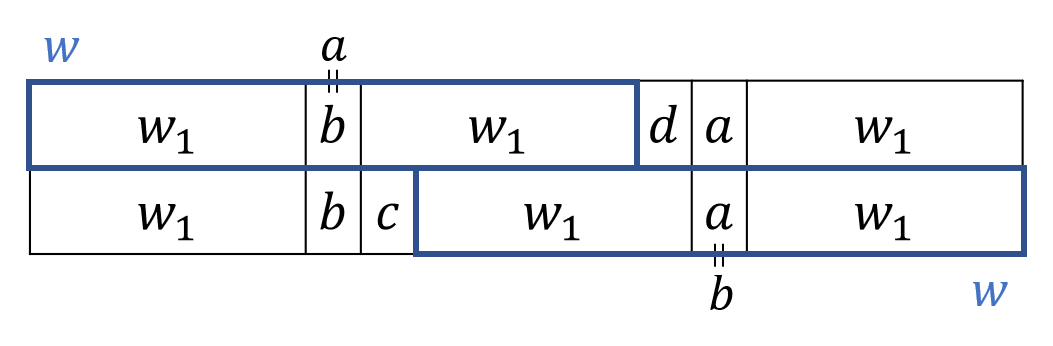
\includegraphics[scale=.4]{画像/追加部分13.png}
\vspace{-.4cm}
\caption{$|w| = 2|w_{1}|+1$における定数記号列}
\label{追加部分13}
\vspace*{.5cm}
%\vspace*{-.4cm}
%\end{figure}
%
%
%\begin{figure}[H]
%\begin{figure}
\centering
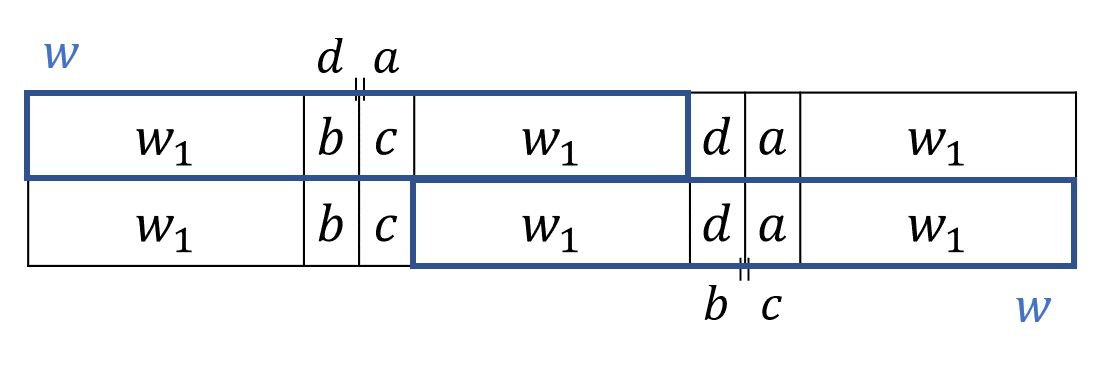
\includegraphics[scale=.4]{画像/追加部分12.png}
\vspace{-.5cm}
\caption{$|w| = 2|w_{1}|+2$における定数記号列}
\label{追加部分12}
\vspace*{.5cm}
%\vspace*{-.4cm}
%\end{figure}
%
%
%\begin{figure}[H]
%\begin{figure} 
\centering
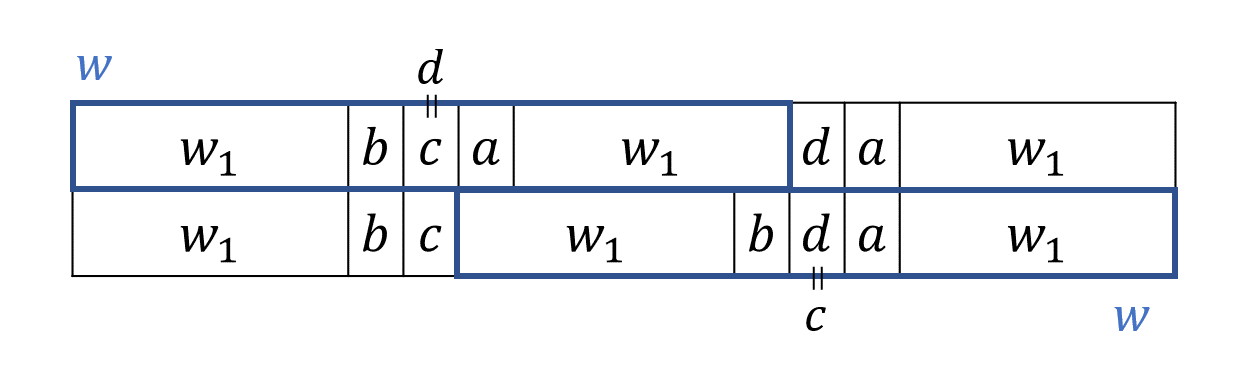
\includegraphics[width=\linewidth]{画像/追加部分11.png}
\vspace{-1cm}
\caption{$|w| = 2|w_{1}|+3$における定数記号列}
\label{追加部分11}
\vspace*{.5cm}
%\vspace*{-.7cm}
%\end{figure}
%
%
%\begin{figure}[H]
%\begin{figure}
\centering
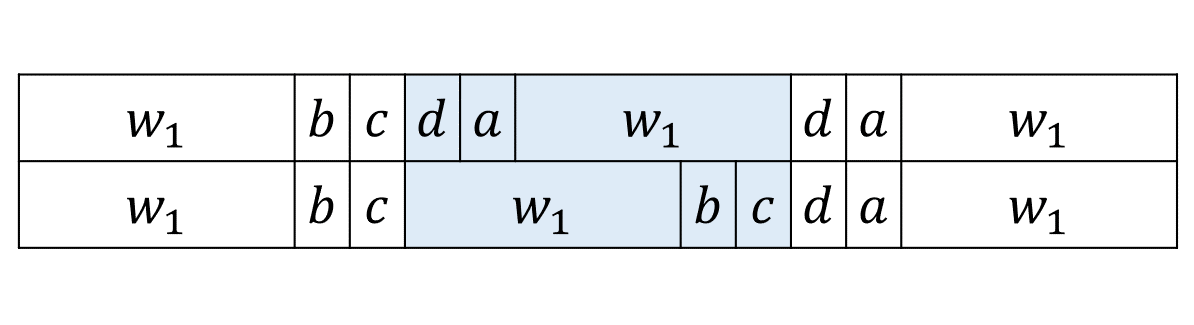
\includegraphics[width=\linewidth]{画像/追加部分10.png}
\vspace{-1.2cm}
\caption{$|w| = 2|w_{1}|+4$における定数記号列}
\label{追加部分10}
%\vspace*{-.5cm}

%\centering
%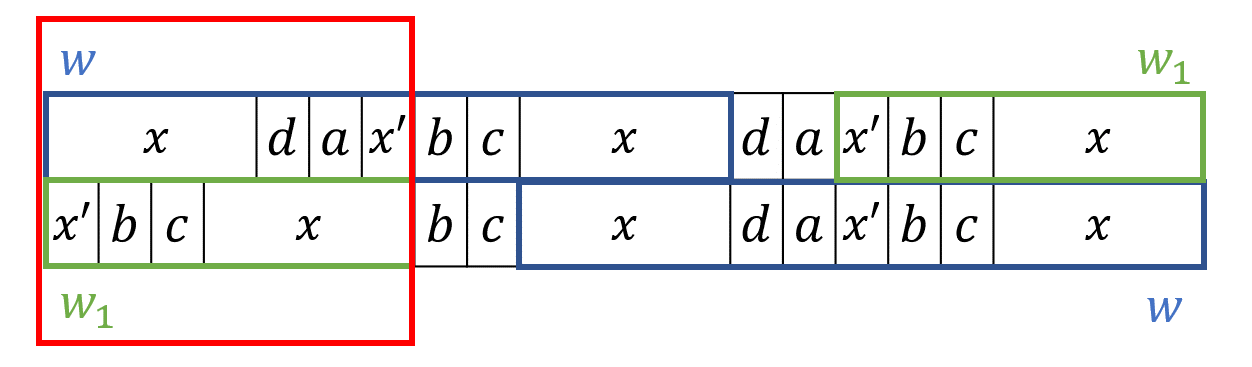
\includegraphics[width=\linewidth]{画像/w1+3.png}
%\vspace{-1cm}
%\caption{$|w_{1}|+3 \le |w| \le 2|w_{1}|-1$における定数記号列}
%\label{w1+3}
\end{figure}

$|w|=2|w_{1}|+4$のとき,$w=w_{1}bcdaw_{1}$とおける.
図\ref{追加部分10}のように,$daw_{1}=w_{1}bc$となる.
これは,主張\ref{主張1}に矛盾する.

\noindent$\textbf{(c)}$ $|w_{1}|=0$のとき,$wda \not = bcw$ $(b \not = a,d$かつ$c \not = a,d)$となる.
これは,主張\ref{主張1}に矛盾する.

上記以外の範囲$\textbf{(d)}$ $|w_{1}|+3 \le |w| \le 2|w_{1}|-1$と$\textbf{(e)}$ $|w| \ge 2|w_{1}|+5$である場合,対象とする定数記号列の長さを減らして考えることができる.

\noindent$\textbf{(d)}$ $|w_{1}|+3 \le |w| \le 2|w_{1}|-1$のとき,

%\begin{figure}[H]
%\begin{figure}
%\centering
%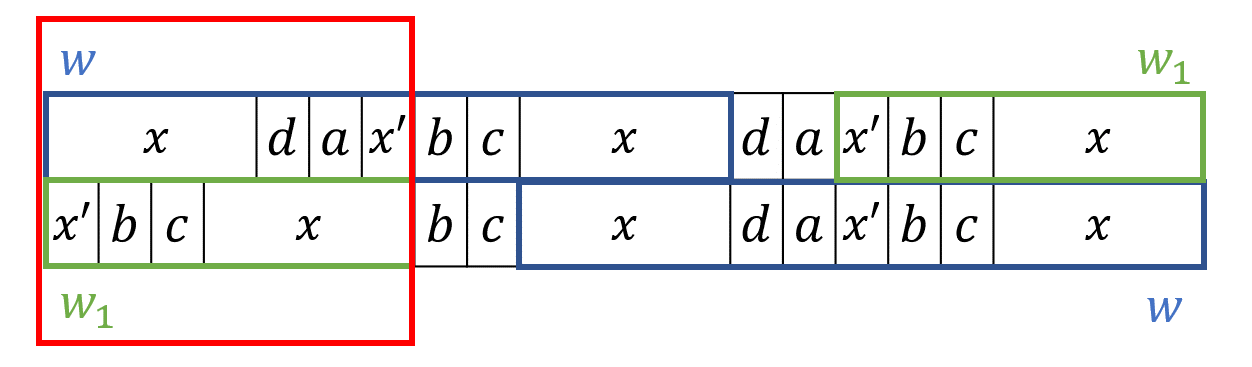
\includegraphics[width=\linewidth]{画像/w1+3.png}
%\vspace{-1cm}
%\caption{$|w_{1}|+3 \le |w| \le 2|w_{1}|-1$における定数記号列}
%\label{w1+3}
%\end{figure}

図\ref{w1+3}のように,$W$を$w$,$W^{\prime}$を$w_{1}$と置き換えて考えることができる.
よって,赤枠部分以外の定数記号列を無視できるため,対象とする定数記号列の長さを減らすことができる.

\noindent$\textbf{(e)}$ $|w| \ge 2|w_{1}|+5$のとき,

%\begin{figure}[H]
\begin{figure}
\centering
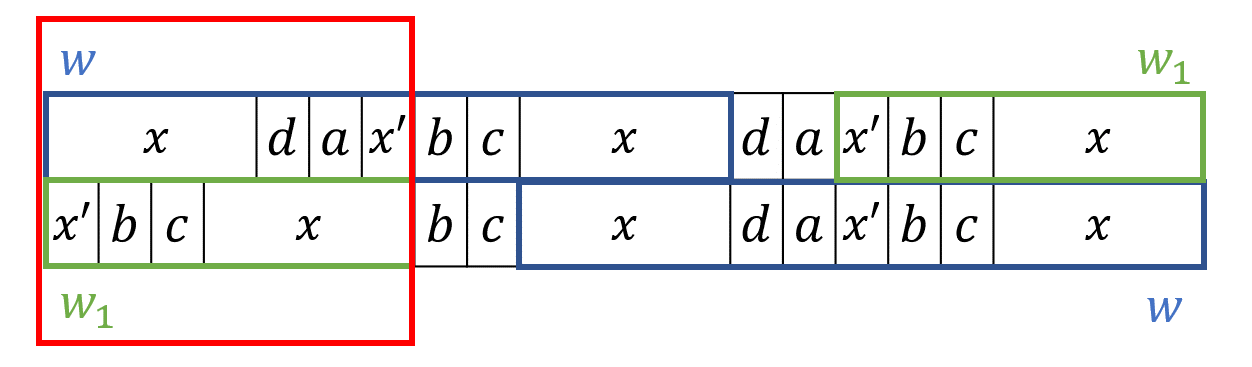
\includegraphics[width=\linewidth]{画像/w1+3.png}
\vspace{-1cm}
\caption{$|w_{1}|+3 \le |w| \le 2|w_{1}|-1$における定数記号列}
\label{w1+3}
%\vspace*{-.3cm}

\centering
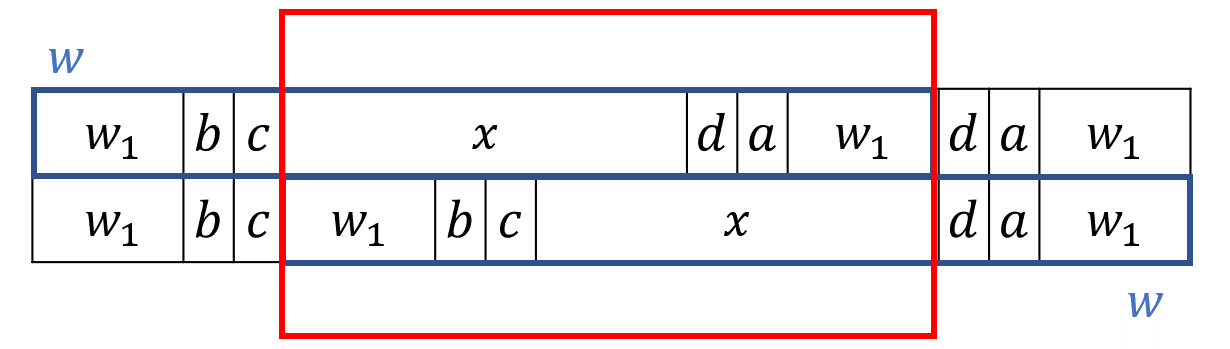
\includegraphics[width=\linewidth]{画像/2w1+5.png}
\vspace{-1cm}
\caption{$|w| \ge 2|w_{1}|+5$における定数記号列}
\label{2w1+5}
\vspace*{-.3cm}
\end{figure}

図\ref{2w1+5}のように,$W$と$w$を置き換えて考えることができる.
よって,赤枠部分以外の定数記号列を無視できるため,対象とする定数記号列の長さを減らすことができる.

したがって,$\textbf{(d)}$ $|w_{1}|+3 \le |w| \le 2|w_{1}|-1$と$\textbf{(e)}$ $|w| \ge 2|w_{1}|+5$の場合,$w,w_{1}$の長さを減らして考えることができる.
この結果より,$w$と$w_{1}$の長さの関係は,最終的に,$\textbf{(a)}$ $|w_{1}| \le |w| \le |w_{1}|+2$,$\textbf{(b)}$ $2|w_{1}| \le |w| \le 2|w_{1}|+4$,$\textbf{(c)}$ $|w_{1}|=0$のいずれかに当てはまるため,仮定に矛盾する.

\hspace{\fill}\rm{(主張\ref{主張2}のQ.E.D)}

よって,$w^{\prime}daw_{1}=w_{1}bcw^{\prime}$は,主張\ref{主張2}に矛盾する.
次に,$|w| < |w^{\prime}|$である場合を考える.

$|w^{\prime}|=|w|+1$のとき,(1')と(2')より,$p_{2}$の接頭辞は$wbcw^{\prime}d$かつ$w^{\prime}d$である.
$|wbc|=|w^{\prime}d|$より,$c=d$となる.
これは,$c \ne d$であることに矛盾する.

$|w^{\prime}|=|w|+2$のとき,(1')と(2')より,$p_{2}$の接頭辞は$wbcw^{\prime}d$かつ$w^{\prime}d$である.
$|wbc|=|w^{\prime}|$より,$w^{\prime}$の最初の記号は$d$となり,$w^{\prime}$の最後の2つの記号は$bc$となる.
(2)と(3)より,$p_{1}$の接尾辞は$awbcw^{\prime}$かつ$aw$であるため,$|w^{\prime}|-1=|aw|$より,$w^{\prime}$の最初から2つ目の記号は$a$となる.
よって,$w^{\prime}=wbc=daw$となる.
これは,主張\ref{主張1}に矛盾する.

$|w^{\prime}| \ge |w|+3$のとき,(1')と(2')より,$p_{2}$の接頭辞は$wbcw^{\prime}d$かつ$w^{\prime}d$である.
$|wbcw_{1}|=|w^{\prime}|$ ($w_{1}$は定数記号列)より,$w^{\prime}$の接頭辞は$w_{1}d$となり,$w^{\prime}$の接尾辞は$bcw_{1}$となる.
(2)と(3)より,$p_{1}$の接尾辞は$awbcw^{\prime}$かつ$aw$である.
$|w^{\prime}|-|w_{1}|-1=|aw|$より,$w^{\prime}$の最初から2つ目の記号は$a$となる.
よって,$w^{\prime}=wbcw_{1}=w_{1}daw$となる.
これは,主張\ref{主張2}に矛盾する.
\end{proof}

\begin{lem}\label{片方}
$\sharp \Sigma \ge 3$とし,$p,~q$を正規パターンとする.
正規パターンの有限集合$D$が,次の{\rm (i), (ii)}のいずれかで表されるとき,すべての$r \in D$に対して$p \{ x := r \} \preceq q$ならば,$p \{ x := xy \} \preceq q$である.

\begin{description}
\item[{\rm (i)}] $\{ ya, bc, dy \}$ $(b = a,c \not = a,d,b \not = d)$,
\item[{\rm (ii)}] $\{ ya, bc, dy \}$ $(b \not = a,d,c = d,c \not = a)$.
\end{description}
\end{lem}
\begin{proof}
$p$に変数記号が現れない場合は自明である.
したがって,$p=p_{1}xp_{2}$ ($p_{1}, p_{2}$は正規パターン, $x$は変数記号)とおく.$p \{ x := xy \} \not \preceq q$と仮定して,矛盾を導く.

\noindent\textbf{(i)}
$D=\{ ya, bc, dy \}$ $(b = a,c \not = a,d,b \not = d)$であるとする.
すべての$r \in D$に対して$p \{ x := r \} \preceq q$であるから
正規パターン$q$には,$ya, bc, dy$に対応する3つの長さ2の記号列が存在する.
その3つの記号列は一部を重複して現れることがあることに注意する.$D$の3つの記号列に対応する$q$の記号列の現れ方には次の3通り存在する.

\begin{description}
\item[(a)] $y_{1}a, bc, dy_{2}$,
\item[(b)] $y_{1}a, y_{2}c, dy_{3}$,
\item[(c)] $y_{1}a, by_{2}, dy_{3}$.
\end{description}

\textbf{(a)}
記号列$A,B,C$に対して,$\{ A,B,C \} = \{ y_{1}a,bc,dy_{2} \}$とおき,$q=q_{1}AwBw^{\prime}Cq_{2}$とする.
これに対して,次の式が成り立っているものとする.
\begin{align*}
(1)~& p_{1} \preceq q_{1} & (1')~& p_{2} \preceq wBw^{\prime}Cq_{2} \\
(2)~& p_{1} \preceq q_{1}Aw & (2')~& p_{2} \preceq w^{\prime}Cq_{2} \\
(3)~& p_{1} \preceq q_{1}AwBw^{\prime} & (3')~& p_{2} \preceq q_{2}
\end{align*}

$q^{\prime}_{1}=q_{1}A,q^{\prime}_{2}=wBw^{\prime},q^{\prime}_{3}=Cq_{2}$とおくと,(3)と(1')より,$p_{1} \preceq q^{\prime}_{1}q^{\prime}_{2},p_{2} \preceq q^{\prime}_{2}q^{\prime}_{3}$となる.
補題\ref{補題9}より,$q^{\prime}_{2}$に変数が含まれるとき,$p \preceq q$となる.
よって,$B=y_{1}a$または,$B=dy_{2}$である場合,仮定に矛盾する.
したがって,$B=bc$である場合のみを考える.

$A=dy_{2}$とすると,(2)は$p_{1} \preceq q_{1}dy_{2}w$となる.
$p_{1}=p^{\prime}_{1}p^{\prime\prime}_{1}, p^{\prime}_{1} \preceq q_{1}d$かつ$p^{\prime\prime}_{1} \preceq y_{2}w$とおくと,(1')より,$p=p_{1}xp_{2}=p^{\prime}_{1}p^{\prime\prime}_{1}xp_{2} \preceq q_{1}dp^{\prime\prime}_{1}xwbcw^{\prime}y_{1}aq_{2}=q \{ x:=p^{\prime\prime}_{1}x \}$となり,$p=q\theta$となる.
これは仮定に矛盾する.
したがって,$A=y_{1}a,B=bc,C=dy_{2}$である場合のみ考えればよい.

以上より,記号列が重複する場合を考慮して,次の2つの場合に分けて証明する.

\begin{description}
\item[(a-1)] $q=q_{1}y_{1}awbcw^{\prime}dy_{2}q_{2}$,
\item[(a-2)] $q=q_{1}y_{1}acwdy_{2}q_{2}$ ($a=b$),
\end{description}

%$p \{ x:=ya \} \preceq q$かつ$p \{ x:=bc \} \preceq q$かつ$p \{ x:=dy \} \preceq q$ならば,
\textbf{(a-1)}
補題\ref{追加部分}の証明より,$p \{ x:= xy \} \preceq q$となる.
よって,仮定に矛盾する.

\textbf{(a-2)}
$q=q_{1}y_{1}acwdy_{2}q_{2}$ ($a=b$)とする.
この$q$に対して,次の式が成り立っているものとする.
\begin{align*}
(1)~& p_{1} \preceq q_{1} & (1')~& p_{2} \preceq cwdy_{2}q_{2} \\
(2)~& p_{1} \preceq q_{1}y_{1} & (2')~& p_{2} \preceq wdy_{2}q_{2} \\
(3)~& p_{1} \preceq q_{1}y_{1}acwdy_{2} & (3')~& p_{2} \preceq q_{2}
\end{align*}

$|w|=0$であれば,(1')と(2')より,$p_{2}$の接頭辞は$cd$かつ$d$となる.
よって,$c=d$となる.
これは,$c \not = d$であることに矛盾する.

$|w|=1$であれば,(1')と(2')より,$p_{2}$の接頭辞は$cwd$かつ$wd$となる.
よって,$w=c=d$となる.
これは,$c \not = d$であることに矛盾する.

$|w| \ge 2$であれば,(1')と(2')より,$p_{2}$の接頭辞は$cwd$かつ$wd$となる.
長さ$n$の$w$を$w_{1}w_{2}w_{3} \cdots w_{n-1}w_{n}$ $(w_{i}$ $(i=1, \ldots , n)は定数記号)$とする.
$cw=wd$より,$w$の接頭辞は$c$,$w$の接尾辞は$d$となる.
よって,$cw_{2}w_{3} \cdots w_{n-1}d$となる.
$cw=ccw_{2}w_{3} \cdots w_{n-1}d,wd=cw_{2}w_{3} \cdots w_{n-1}dd$であるから,$cw=wd$より,$w_{i}=w_{i+1}$ $(i=2, \ldots , n-2)$となる.
したがって,$c=d$となる.
これは,$c \not = d$であることに矛盾する.

\textbf{(b)}の記号列を含む正規パターン$q$は,
$c \not = a$より,補題\ref{変数2つ}(i-2)に対応する記号列が現れる.
よって,$p \{ x:= xy \} \preceq q$となる.
これは,仮定に矛盾する.

\textbf{(c)}の記号列を含む正規パターン$q$は,
$b \not = d$より,補題\ref{変数2つ}(i-1)に対応する記号列が現れる.
よって,$p \{ x:= xy \} \preceq q$となる.

\noindent\textbf{(ii)}
$D=\{ ya, bc, dy \} \ (b \not = a,d,c = d$かつ$c \not = a)$のときは,記号列$p$と$q$を逆順にすることにより,\textbf{(ii)}の場合と同様に, 仮定$p \{ x := xy \} \not\preceq q$に矛盾することを証明できる.
\end{proof}

補題\ref{追加部分},補題\ref{片方}より,次の系が得られる.

\begin{col}\label{両方}
$\sharp \Sigma \ge 3$とし,$p, q$を正規パターンとする.
正規パターンの有限集合$D= \{ ya, bc, dy \}$ $(b = a$かつ$c = d)$で表されるとき,任意の$r \in D$に対して$p \{ x := r \} \preceq q$ならば,$p \{ x := xy \} \not \preceq q$となる$q$が存在する.
\end{col}
\begin{ex}
$a,b,c,d,e$を定数記号,$x,y,y_{1},y_{2}$を変数記号とする.
$p \{ x:=xy \} \not \preceq q$となる正規パターン$p,q$を$p=eabcbcadabcbcadaxbcadadabcbcadade,q=y_{1}abcbcadabcbcadady_{2}$ $(b = a$かつ$c = d)$とする.
\end{ex}

%\begin{figure}[H]
\begin{figure}
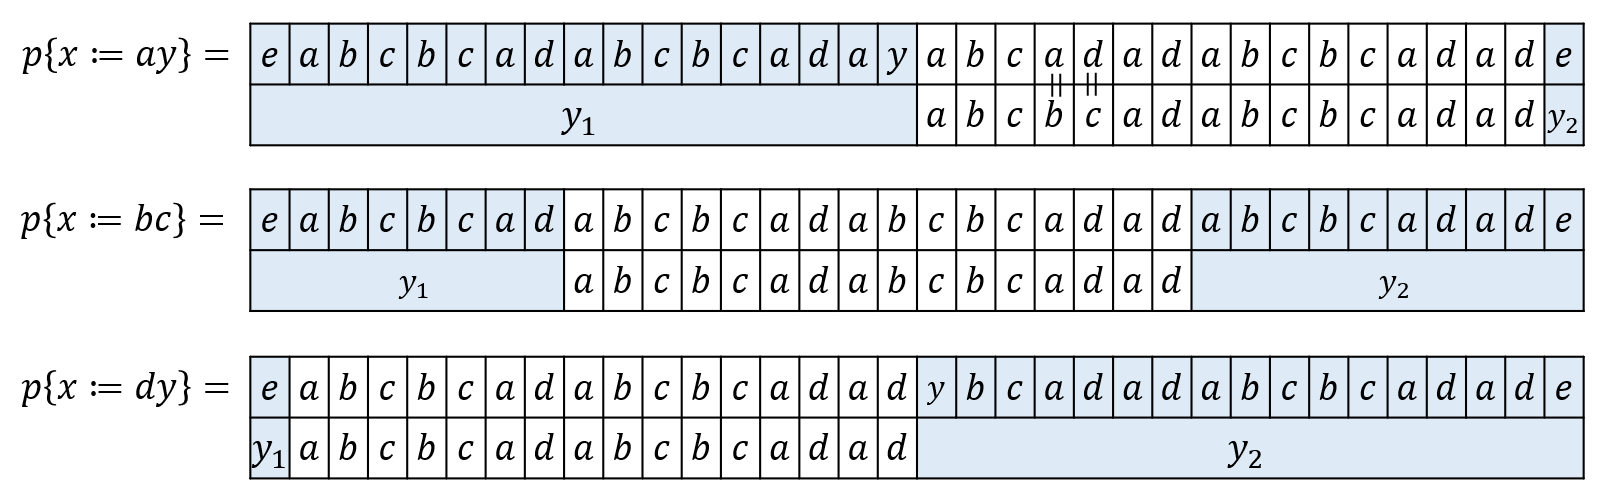
\includegraphics[width=\linewidth]{画像/b=aとc=dの例.png}
\vspace{-1cm}
\caption{$p$に対する代入と$q$の関係}
\label{b=aとc=dの例}
\end{figure}

このとき,図\ref{b=aとc=dの例}のように,
\begin{eqnarray*}
&p& \{ x:=ya \} \\ 
& = & (eabcbcadabcbcaday)abcadadabcbcadade\\
& = & q \{ y_{1} := eabcbcadabcbcaday_{1} \} \\
& \preceq & q,\\
&p& \{ x:=bc \}  \\
& = & (eabcbcad)abcbcadabcbcadad(abcbcadade) \\
& = & q \{ y_{1} := eabcbcad,y_{2} := abcbcadade \} \\
& \preceq & q,\\
&p& \{ x:=dy \}  \\
& = & eabcbcadabcbcadad(ybcadadabcbcadade) \\
& = & q \{ y_{2} := y_{2}bcadadabcbcadade \} \\
& \preceq & q.
\end{eqnarray*}
となる.
これは,系\ref{両方}の条件を満たす.
\begin{comment}
\begin{lem}\label{追加補題2}
$\sharp \Sigma \ge 3$とし,$p, q$を正規パターンとする.
正規パターンの有限集合$D= \{ ya,ab,by,cd \}$ $(cd \not = ab)$で表されるとき,すべての$r \in D$に対して$p \{ x := r \} \preceq q$ならば,$p \{ x := xy \} \preceq q$である.
\end{lem}
\begin{proof}
$p$に変数記号が現れない場合は自明である.
したがって,$p=p_{1}xp_{2}$ ($p_{1}, p_{2}$は正規パターン, $x$は変数記号)とおく.$p \{ x := xy \} \not \preceq q$と仮定して,矛盾を導く.

$c \not = a$かつ$d \not = b$であるとき,系\ref{両方}より,$p \{ x:= xy \} \preceq q$となる.
これは,仮定に矛盾する.

$c \not = a$かつ$d = b$,または,$c = a$かつ$d \not = b$であるとき,補題\ref{片方}より,$p \{ x:=xy \} \preceq q$となる.
これは,仮定に矛盾する.
\end{proof} 
\end{comment}
%\begin{lem}\label{追加補題1}
%$k \ge 3$,$m \ge \sqrt{k+1}$,$\sharp \Sigma \ge k+m$,$P \in \RPatplus$,$Q \in \RPat^{k}$とする.
%すべての定数記号$a, b \in \Sigma$に対し,ある正規パターン$q \in Q$が存在し,
%$p \{ x:=ab \} \preceq q$ならば,$p \{ x:=xy \} \preceq q$となる.
%\end{lem}

\begin{lem}\label{追加補題1}
$\sharp \Sigma \ge k+2$,$p \in \RPat$,$Q \in \RPat^{k}$とする.
任意の定数記号$a, b \in \Sigma$に対し,ある正規パターン$q \in Q$が存在し,
$p \{ x:=ab \} \preceq q$ならば,$p \{ x:=xy \} \preceq q$となる.
\end{lem}
\begin{proof}
$p$に変数記号が現れない場合は自明である.
したがって,$p=p_{1}xp_{2}$ ($p_{1},p_{2}$は正規パターン,$x$は変数記号)とおく.
また,$Q=\{ q_{1}, \ldots , q_{k} \}$とする.次のように記号を定める.
\begin{align*}
& A_{i} = \{ a \in \Sigma \mid p \{ x:=ay \} \preceq q_{i},\ y\in X\},\\ 
& B_{i} = \{ b \in \Sigma \mid p \{ x:=yb \} \preceq q_{i},\ y\in X\},\\ 
%& \tilde{B}_{i} = \{ \tilde{b} \in \Sigma \mid p \{ x:=yb \} \preceq q_{i},\ y\in X\},\\ 
& A = \bigcup_{i=1}^{k}A_{i},B = \bigcup_{i=1}^{k} B_{i},\\
& \tilde{B} = \{ \tilde{b} \mid b \in B \},\\
& A^{\prime} = \Sigma\setminus A,B^{\prime} = \Sigma\setminus B,\\
& \tilde{\Sigma} = \{ \tilde{c} \mid c \in \Sigma \},\\
& \tilde{B}^{\prime} = \{ b \mid b \in \tilde{\Sigma} \setminus \tilde{B} \}~~(i=1, \ldots , k).
\end{align*}

$p \{ x:=xy \} \not \preceq q_{i}$ \ ($i=1, \ldots , k$)と仮定する.

$k=1$のとき,$p \{ x:=a_{1}a_{i} \} \preceq q_{1}$かつ$p \{ x:=a_{2}a_{i} \} \preceq q_{1}$ ($i=1,2,3$)となる.
$p^{\prime} = p \{ x:=a_{1}y \} = p_{1}a_{1}yp_{2}$とおくと,$p \{ x:=a_{1}a_{i} \} \preceq q_{1}$より,$p^{\prime} \{ y:=a_{i} \} \preceq q_{1}$となる.
$a_{i}$は互いに異なる定数記号であるため,補題\ref{補題10}より,$p^{\prime} \preceq q_{1}$となる.
よって,$p \{ x:=a_{1}y \} \preceq q_{1}$となる.
$p \{ x:=a_{2}y \}$についても同様に考えることができ,$p \{ x:=a_{2}y \} \preceq q_{1}$となる.
したがって,$p \{ x:=a_{1}y \} \preceq q_{1}$かつ$p \{ x:=a_{2}y \} \preceq q_{1}$であるため,補題\ref{変数2つ}より,$p \{ x:= xy \} \preceq q_{1}$となる.
これは,仮定に矛盾する.

$k \ge 2$のとき,2部グラフを用いて矛盾を導く.
$G=(\Sigma,\tilde{\Sigma}; A^{\prime} \times \tilde{B}^{\prime})$
を$\Sigma$と$\tilde{\Sigma}$を部集合とし,$A^{\prime} \times \tilde{B}^{\prime}$を辺集合とする2部グラフとする.
$\Sigma$と$\tilde{\Sigma}$を部集合とし,$\tilde{E}_{i}=\{ (a, \tilde{b}) \in A^{\prime} \times \tilde{B}^{\prime} \mid p \{ x:=ab \} \preceq q_{i} \}$を辺集合とする2部グラフを$\tilde{G}_{i}=(\Sigma,\tilde{\Sigma}; \tilde{E}_{i})$とする.

$\sharp A_{i} \ge 2$または$\sharp B_{i} \ge 2$となる$i$が存在するとき,補題\ref{変数2つ}より,$p \{ x:=xy \} \preceq q_{i}$となる.
これは仮定に矛盾する.よって,任意の$i$ ($i=1, \ldots , k$)に対して,$\sharp A_{i} \le 1$かつ$\sharp B_{i} \le 1$となる.
また,$0 \le \sharp A \le k$かつ$0 \le \sharp\tilde{B} \le k$となり,$2 \le \sharp A^{\prime} \le k+2$かつ$2 \le \sharp \tilde{B}^{\prime} \le k+2$となる.
$\sharp A=k$かつ$\sharp \tilde{B}=k$である$G$を$G^{(k,k)}$と表し,$\sharp A_{i}=1$かつ$\sharp B_{i}=1$である$\tilde{G}_{i}$を$\tilde{G}^{(1,1)}_{i}$と表す.

$\sharp A$と$\sharp \tilde{B}$の関係を,次の3つの場合に分けて証明する.
\[
\begin{tabular}{ll}
$\textbf{(1)}$ $\sharp A=k$かつ$\sharp \tilde{B} \le k$,\\
$\textbf{(2)}$ $\sharp A = k-1$かつ$\sharp \tilde{B} \le k-1$,\\
$\textbf{(3)}$ $\sharp A \le k-2$かつ$\sharp \tilde{B} \le k-2$.
\end{tabular}
\]
\begin{figure*}
\centering
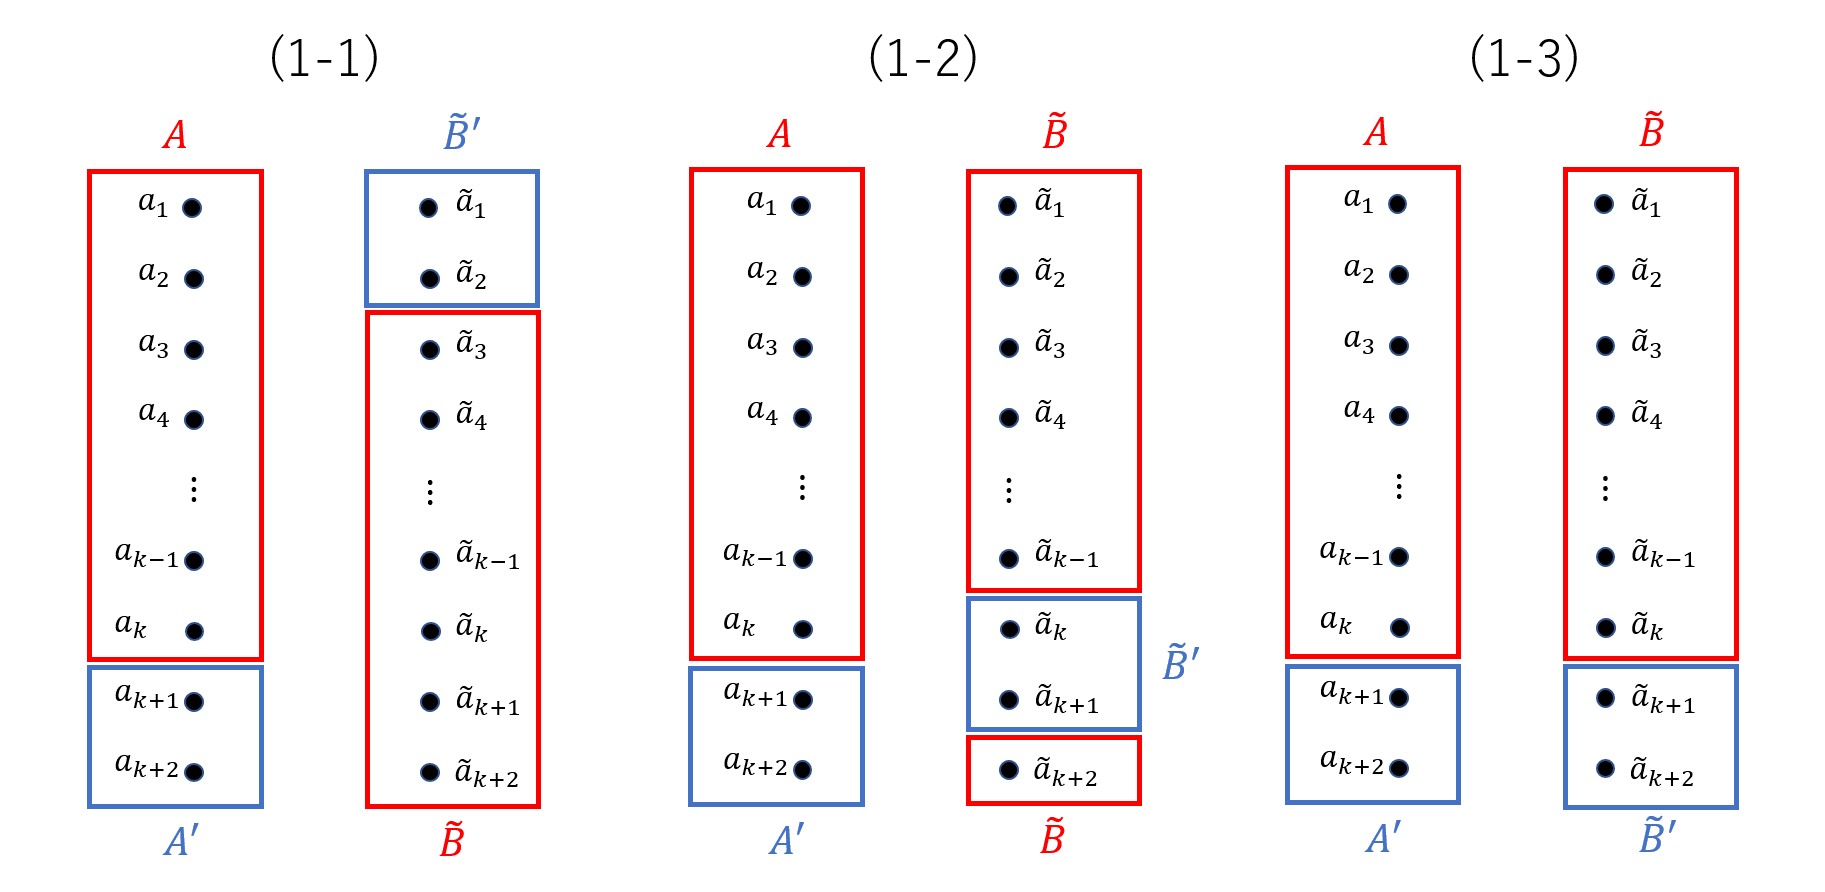
\includegraphics[width=\linewidth]{画像/グラフ比較.png}
\vspace{-1cm}
\caption{(1-1),(1-2),(1-3)の例}
\label{グラフ比較}
\end{figure*}

\noindent\textbf{(1)} 
$\sharp A=k$かつ$\sharp \tilde{B} \le k$であるとき,$\sharp A^{\prime}=2$かつ$\sharp \tilde{B}^{\prime} \ge 2$となる.
このとき,$G$には少なくとも$\sharp A^{\prime} \times \sharp \tilde{B}^{\prime}=2\times2=4$本の辺が含まれる.
図\ref{グラフ比較}のように,$| A^{\prime} \cap B^{\prime} |$の関係は,3種類に分けられる.
よって,以下のように,場合分けして証明する.
\[
\begin{tabular}{ll}
$\textbf{(1-1)}$ $| A^{\prime} \cap B^{\prime} | = 0$,$\textbf{(1-2)}$ $| A^{\prime} \cap B^{\prime} | = 1$,\\
$\textbf{(1-3)}$ $| A^{\prime} \cap B^{\prime} | = 2$.
\end{tabular}
\]

\textbf{(1-1)} 
$\sharp A = k$かつ$\sharp \tilde{B} = k$であるとき,
$p \{ x:=ya_{i} \} \preceq q_{i}$かつ$p \{ x:=a_{i}y \} \preceq q_{i}$ $(i=3,\ldots,k)$とし,$p \{ x:=a_{j}y \} \preceq q_{j}$かつ$p \{ x:=ya_{k+j} \} \preceq q_{j}$ $(j=1,2)$とする.

%\begin{figure}[H]
\begin{figure}  
\centering
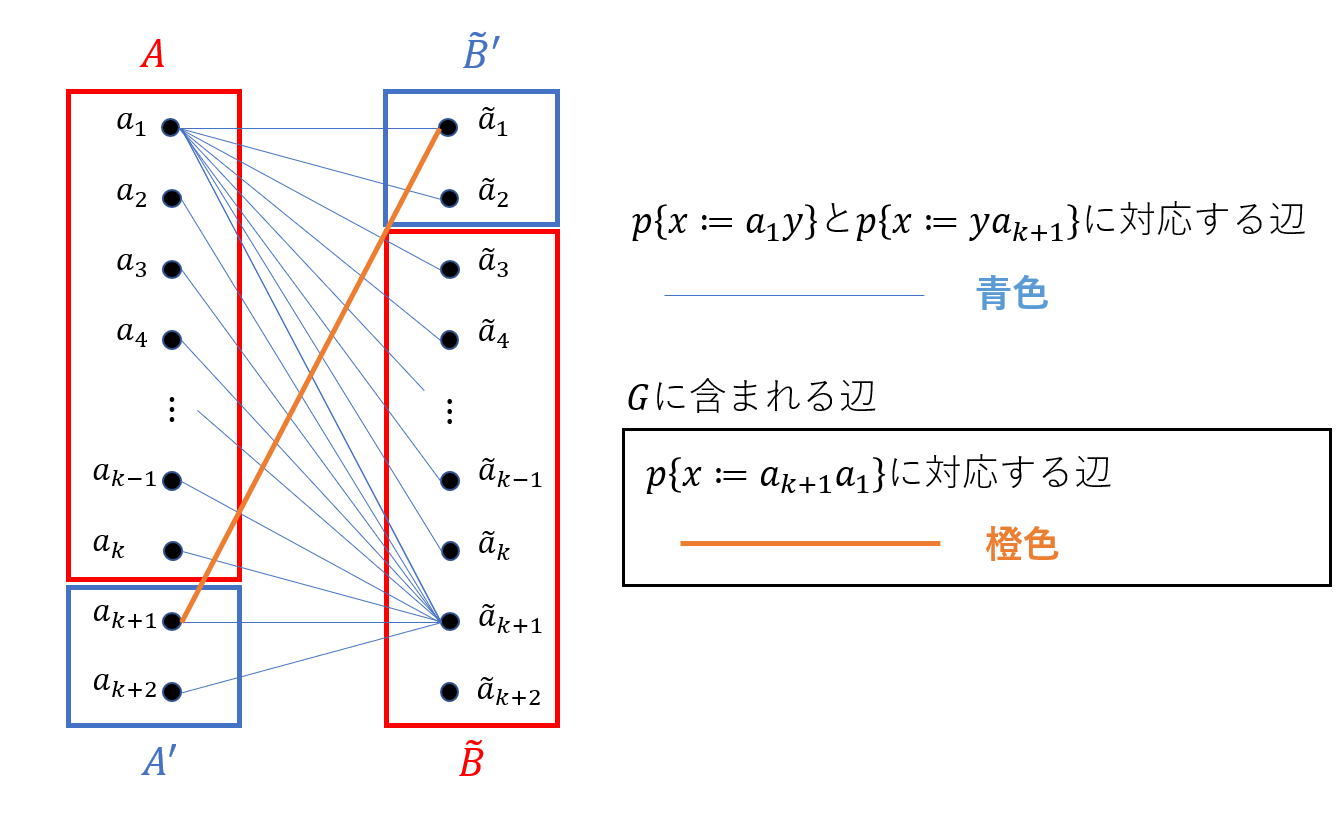
\includegraphics[width=\linewidth]{画像/系との関係.png}
\vspace{-1cm}
\caption{系\ref{両方}の条件に当てはまるパターンにおける二分グラフの例}
\label{系との関係}
%\vspace*{-.5cm}
\end{figure}

系\ref{両方}より,$p \{ x:=a_{k+1}a_{1} \} \preceq q_{1}$(図\ref{系との関係}),$p \{ x:=a_{k+2}a_{2} \} \preceq q_{2}$となる$q_{1},q_{2}$が考えられる.

このとき,$\tilde{G}_{1}$と$\tilde{G}_{2}$に含まれる辺はそれぞれ1本となる.
$G$に含まれる辺は,4本であるため,残り$4-2=2$本の辺は$\tilde{G}_{i}$ $(i=3, \ldots, k)$に含まれる.
すなわち,$p \{ x:=a_{k+1}a_{2} \} \preceq q_{i_{0}}$と$p \{ x:=a_{k+2}a_{1} \} \preceq q_{i_{1}}$となる$q_{i_{0}}$と$q_{i_{1}}$が存在する.
任意の$i$ $(i=3, \ldots, k)$に対して,$p \{ x:=ya_{i} \} \preceq q_{i}$かつ$p \{ x:=a_{i}y \} \preceq q_{i}$であるため,$q_{i_{0}},q_{i_{1}} \in Q \setminus \{ q_{1},q_{2} \}$より,$a_{k+1} \not = a_{i}$かつ$a_{2} \not = a_{i}$となる.
よって,補題\ref{追加部分}より,$p \{ x:=xy \} \preceq q_{i_{0}}$となり,仮定に矛盾する.

$\sharp A = k$かつ$\sharp \tilde{B} < k$であるとき,$\sharp A_{i}=1$かつ$\sharp B_{i}=0$となる$i$が存在する.

%\begin{figure}[H]
\begin{figure}
\centering
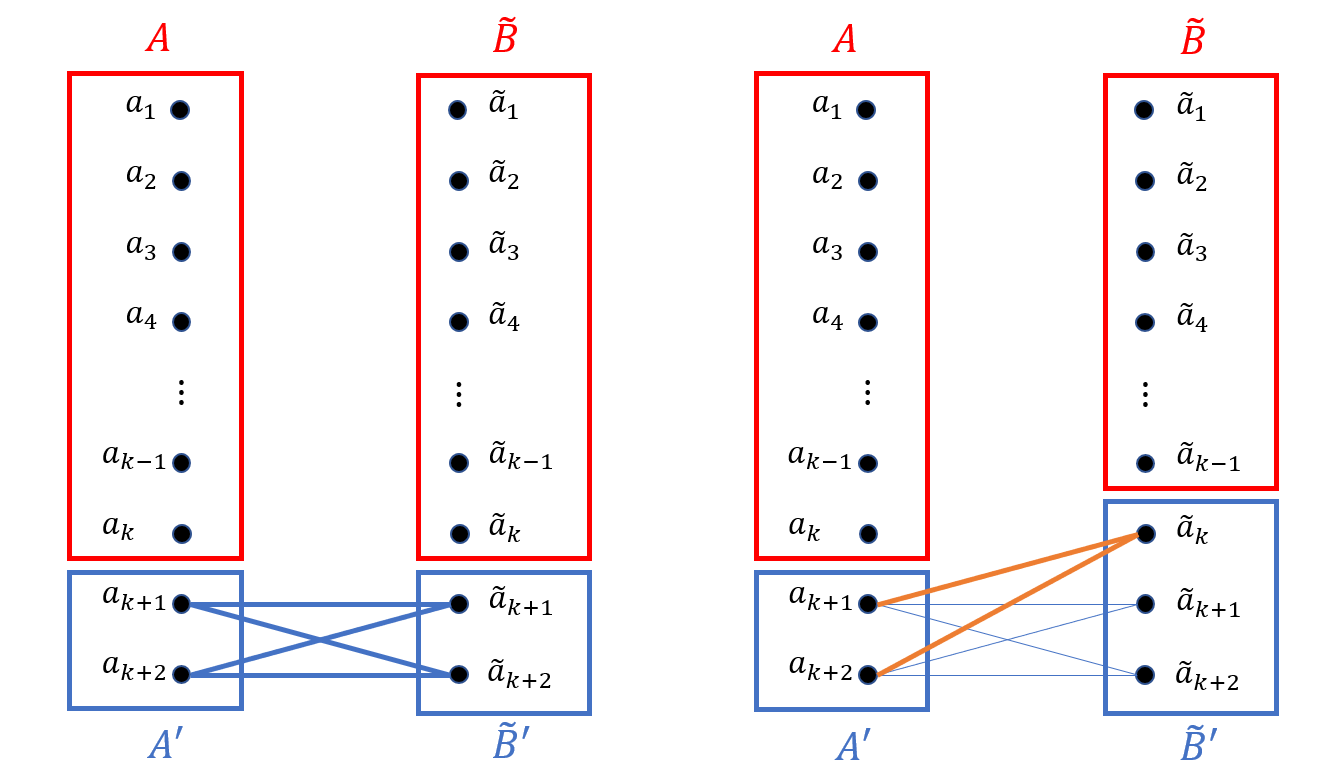
\includegraphics[width=\linewidth]{画像/abが異なる場合.png}
\vspace{-1cm}
\caption{$\sharp A_{k} =1$かつ$\sharp B_{k}=1$の場合と$\sharp A_{k}=1$かつ$\sharp B_{k}=0$の場合の$G$に含まれる辺数の違い}
\label{abが異なる場合}
\end{figure}

図\ref{abが異なる場合}のように,$G^{(k,k-1)}$に含まれる辺の本数は,$G^{(k,k)}$と比べて,$\sharp A^{\prime}$本多くなる.
すなわち,ある$\tilde{G}^{(1,1)}_{i}$が$\tilde{G}^{(1,0)}_{i}$となった場合,全体の$G$に含まれる辺の本数は,$\sharp A^{\prime}$本多くなる.
このことから,$G^{(k,k-1)}$の部分グラフ$\tilde{G}^{(1,0)}_{i}$に含まれる辺の本数が$\sharp A^{\prime}$本以下であるとき,$G^{(k,k)}$における結果と同様となる.
一方で,$G^{(k,k-1)}$の部分グラフ$\tilde{G}^{(1,0)}_{i}$に$\sharp A^{\prime}+1=2+1=3$本以上の辺が含まれるとき,$G^{(k,k)}$における結果から変化する可能性がある.

$G^{(k,k-2)}$の部分グラフ$\tilde{G}^{(1,0)}_{i_{0}}$と$\tilde{G}^{(1,0)}_{i_{1}}$が,それぞれ$3$本の辺を含むとき,以下のような例が考えられる.

\begin{ex}\label{少なくなるとき}
${G}^{(k,k-2)}$の部分グラフ$\tilde{G}^{(1,0)}_{k-1}$と$\tilde{G}^{(1,0)}_{k}$に$\sharp A^{\prime}+1=2+1=3$本の辺が含まれるとき,
\begin{description}
\item[$(\mathrm{i})$] $p \{ x:= a_{i}y \} \preceq q_{i}$かつ$p \{ x:= ya_{i} \} \preceq q_{i}$ $(i=3, \ldots , k-2)$,
\item[$(\mathrm{ii})$] $p \{ x:=a_{j}y \} \preceq q_{j},p \{ x:=ya_{k+j} \} \preceq q_{j}$かつ$p \{ x:=a_{k+j}a_{j} \} \preceq q_{j}$ $(j=1,2)$,
\item[$(\mathrm{iii})$] $p \{ x:=a_{k-1}y \} \preceq q_{k-1},p \{ x:=a_{z}a_{k-1} \} \preceq q_{k-1}$かつ$p \{ x:=a_{1}a_{k+2} \} \preceq q_{k-1}$ \\$(z=k+1,k+2)$,
\item[$(\mathrm{iv})$] $p \{ x:=a_{k}y \} \preceq q_{k},p \{ x:=a_{z}a_{k} \} \preceq q_{k}$かつ$p \{ x:=a_{2}a_{k+1} \} \preceq q_{k}$.
\end{description}
となる$p$と$q_{i}$ $(i=1,\ldots,k)$が存在し,$p \{ x:=xy \} \not \preceq q_{i}$となる.
\end{ex}
%例\ref{少なくなるとき}において,$G^{(k,k)}$の部分グラフ$\tilde{G}_{i},\tilde{G}_{j}$と$G^{(k,k-2)}$の部分グラフ$\tilde{G}_{i},\tilde{G}_{j}$に含まれる辺数は変わらない.
%よって,$\tilde{G}_{k-1}$と$\tilde{G}_{k}$に注目すればよい.
%$G^{(k,k)}$には$2 \times 2=4$本の辺が含まれ,$G^{(k,k-2)}$には$2 \times 4=8$本の辺が含まれる.
%$\sharp ((\tilde{A} \times \tilde{B}) \setminus E_{i})$は,$G^{(k,k)}$に含まれる辺の$\sharp (\tilde{A} \times \tilde{B})=4$本より少なくなる.
%(1)の場合,$\sharp\tilde{A} = 2$より,$\tilde{G}^{(1,0)}_{i}$に$2+1=3$本以上の辺が含まれるとき,$\sharp ((\tilde{A} \times \tilde{B}) \setminus E_{i})$は,$G^{(k,k)}$に含まれる辺の$\sharp (\tilde{A} \times \tilde{B})$本より少なくなる.
%$\tilde{G}^{(1,0)}_{k-1}$と$\tilde{G}^{(1,0)}_{k}$が,それぞれ$\sharp A^{\prime}+1$=3本の辺を持つ場合,$\tilde{G}_{i}$には辺は含まれない.
%よって,$p \{ x:=xy \} \not \preceq q_{i}$ $(i=1,\ldots,k)$となる.

%\begin{figure}[H]
\begin{figure}
\centering
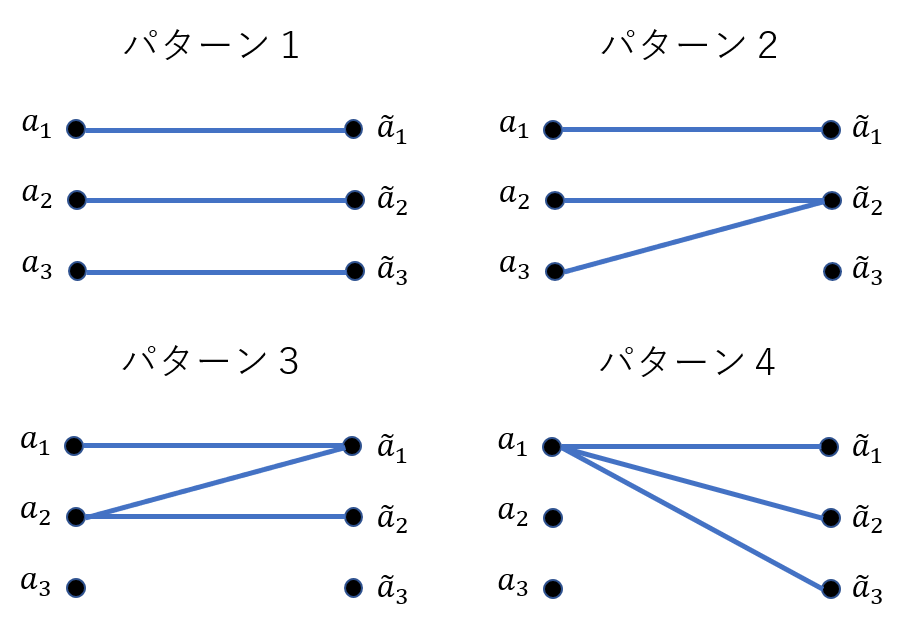
\includegraphics[width=\linewidth]{画像/辺3におけるパターン.png}
\vspace*{-1cm}
\caption{辺数が3である二分グラフの例}
\label{辺3におけるパターン}
\end{figure}

図\ref{辺3におけるパターン}のように,$\tilde{G}^{(1,0)}_{i}$に3本の辺が含まれるパターンは,4つ存在する.
パターン1の場合,補題\ref{補題14}(abc)より,$p \{ x:=xy \} \preceq q_{i}$となる.
パターン2とパターン3の場合,互いに隣接しない辺が2本存在するため,
補題\ref{補題14}(d)より,$p \{ x:=xy \} \preceq q_{i}$となる.
パターン4の場合,$p \{ x:=a_{1}a_{j} \} \preceq q_{i}$ $(j=1,2,3)$となる.
$p^{\prime} = p \{ x:=a_{1}y \} = p_{1}a_{1}yp_{2}$とおくと,$p \{ x:=a_{1}a_{j} \} \preceq q_{i}$より,$p^{\prime} \{ y:=a_{j} \} \preceq q_{i}$となる.
$a_{j}$は互いに異なる定数記号であるため,補題\ref{補題10}より,$p^{\prime} \preceq q_{i}$となり,$p \{ x:=a_{1}y \} \preceq q_{i}$となる.
これは,$A_{i}$の定義に矛盾する.
よって,$\tilde{G}^{(1,0)}_{i}$に含まれる辺は2本以下となる.
したがって,例\ref{少なくなるとき}は,$\tilde{G}^{(1,0)}_{k-1}$と$\tilde{G}^{(1,0)}_{k}$に含まれる辺がそれぞれ2本以下であることに矛盾する.

以上より,$G^{(k,k)}$において,仮定に矛盾する場合,$\sharp A=k$かつ$\sharp \tilde{B}^{\prime} < k$である場合においても,仮定に矛盾する.
(2),(3)のいずれの場合においても,$\sharp A^{\prime} > 2$であることから,同様のことが言える.

\textbf{(1-2)} 
$\sharp A = k$かつ$\sharp \tilde{B} = k$であるとき,
$p \{ x:=ya_{i} \} \preceq q_{i}$かつ$p \{ x:=a_{i}y \} \preceq q_{i}$ $(i=1,\ldots,k-1)$とし,$p \{ x:= ya_{k+2} \} \preceq q_{k}$かつ$p \{ x:= a_{k}y \} \preceq q_{k}$とする.
系\ref{両方}より,$p \{ x:=a_{k+2}a_{k} \} \preceq q_{k}$である$q_{k}$が考えられる.
このとき,$\tilde{G}_{k}$に含まれる辺は1本となる.
$G$に含まれる辺は,4本であるから,残り$4-1=3$本の辺は$\tilde{G}_{i}$ $(i=1, \ldots, k-1)$に含まれる.
すなわち,$p \{ x:=a_{k+1}a_{k+1} \} \preceq q_{i_{0}}$が存在する.
任意の$i$ $(i=1, \ldots, k-1)$に対して,$p \{ x:=ya_{i} \} \preceq q_{i}$かつ$p \{ x:=a_{i}y \} \preceq q_{i}$であるため,$q_{i_{0}} \in Q \setminus \{ q_{k} \}$より,$a_{k+1} \not = a_{i}$となる.
よって,補題\ref{追加部分}より,$p \{ x:=xy \} \preceq q_{i_{0}}$となり,仮定に矛盾する.

\textbf{(1-3)} 
$\sharp A = k$かつ$\sharp \tilde{B} = k$であるとき,
$p \{ x:=ya_{i} \} \preceq q_{i}$かつ$p \{ x:=a_{i}y \} \preceq q_{i}$ $(i=1,\ldots,k)$とする
$G$に$4$本の辺が含まれるため,$p \{ x:=a_{k+1}a_{k+1} \} \preceq q_{i_{0}}$が存在する.
よって,任意の$i$に対して,$a_{k+1} \not = a_{i}$となる.
補題\ref{追加部分}より,$p \{ x:=xy \} \preceq q_{i_{0}}$となり,仮定に矛盾する.

\begin{figure*}
\centering
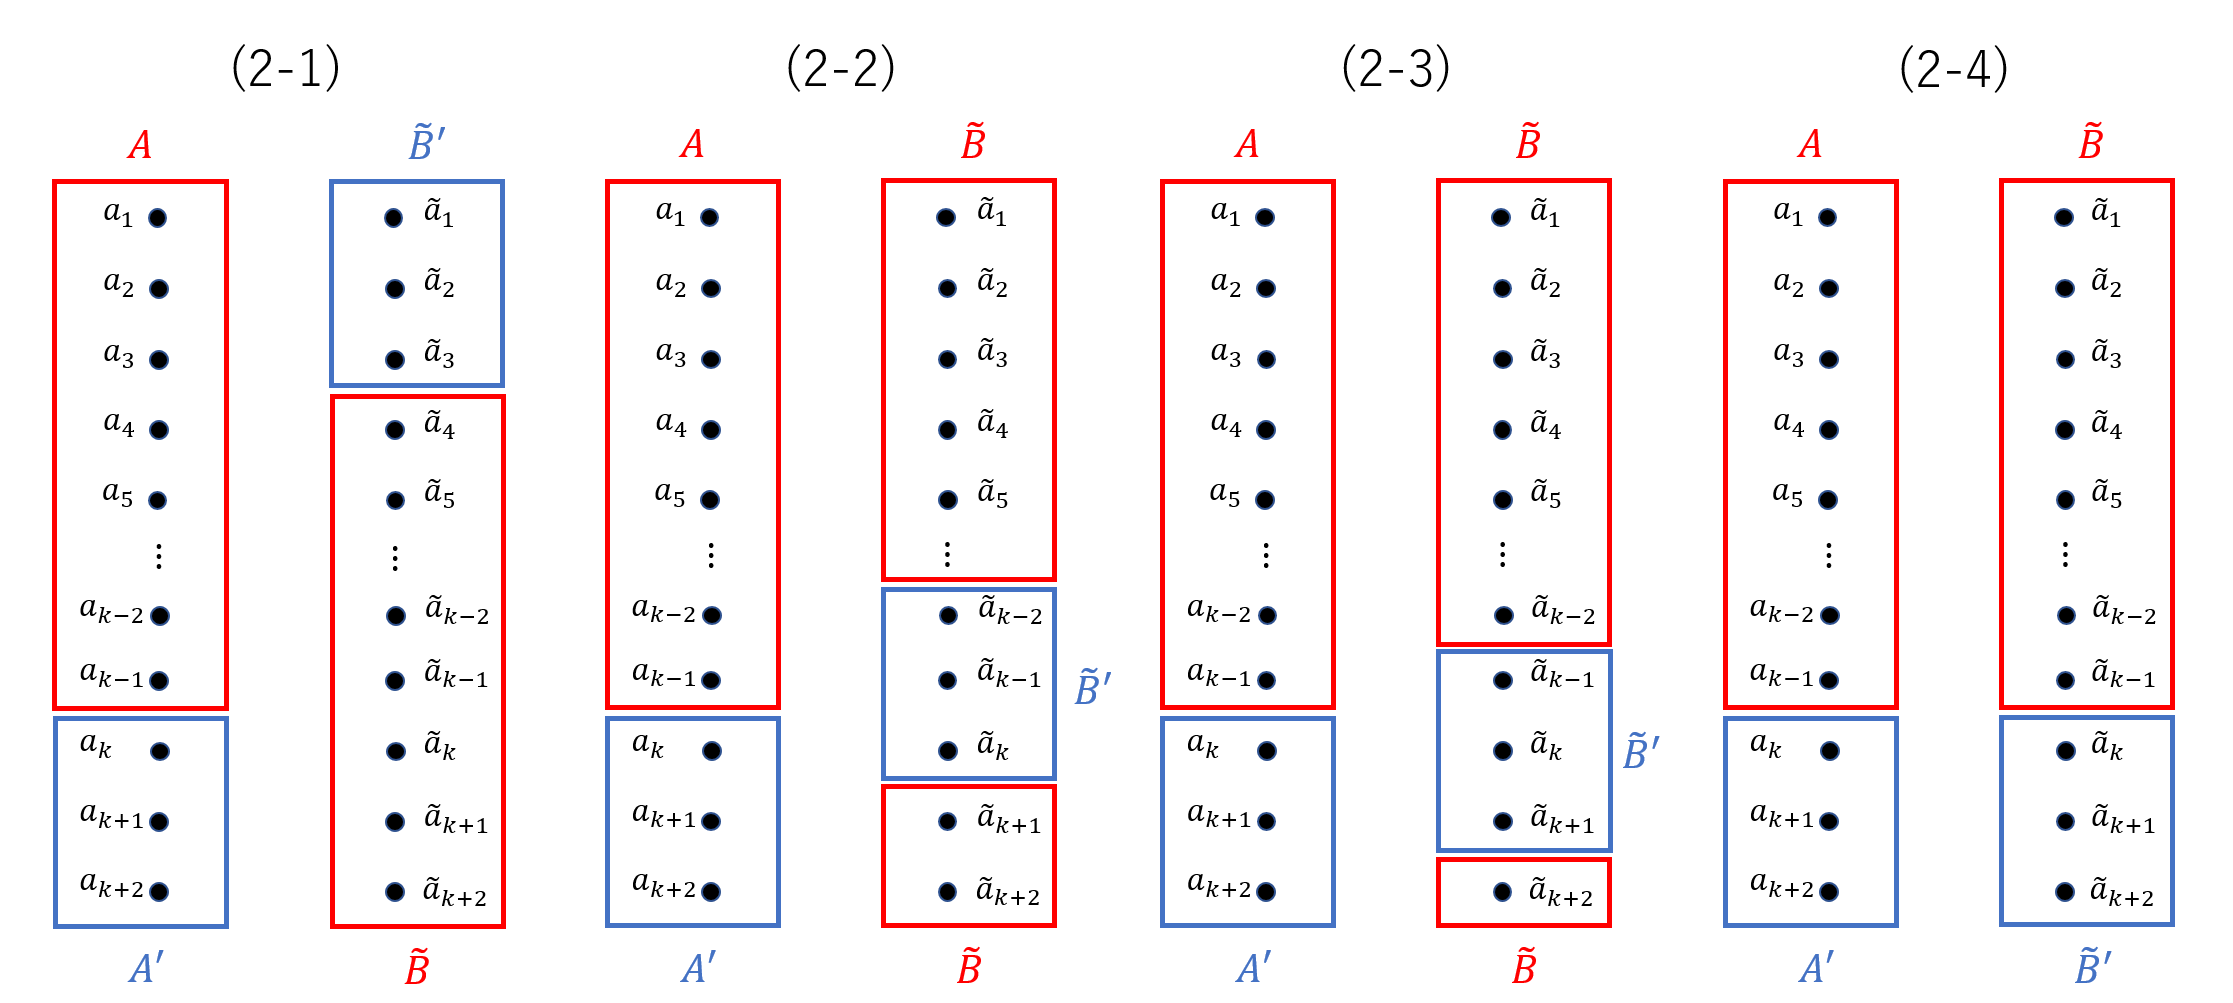
\includegraphics[width=\linewidth]{画像/(2)におけるパターン.png}
\vspace*{-1cm}
\caption{(2-1),(2-2),(2-3),(2-4)の例}
\label{(2)におけるパターン}
\end{figure*}

\noindent\textbf{(2)} 
$\sharp A=k-1$かつ$\sharp B \le k-1$であるとき,$\sharp A^{\prime}=3$かつ$\sharp \tilde{B}^{\prime} \ge 3$となる.
$G$には少なくとも$\sharp A^{\prime} \times \sharp \tilde{B}^{\prime}=3\times3=9$本の辺が含まれる.
図\ref{(2)におけるパターン}のように,$| A^{\prime} \cap B^{\prime} |$の関係は,4種類に分けられる.よって,以下のように,場合分けして証明する.
\[
\begin{tabular}{ll}
$\textbf{(2-1)}$ $| A^{\prime} \cap B^{\prime} | = 0$,$\textbf{(2-2)}$ $| A^{\prime} \cap B^{\prime} | = 1$,\\
$\textbf{(2-3)}$ $| A^{\prime} \cap B^{\prime} | = 2$,$\textbf{(2-4)}$ $| A^{\prime} \cap B^{\prime} | = 3$.
\end{tabular}
\]

\textbf{(2-1)} 
$\sharp A=k-1$かつ$\sharp \tilde{B}=k-1$であるとき,
$p \{ x:=ya_{i} \} \preceq q_{i}$かつ$p \{ x:=a_{i}y \} \preceq q_{i}$ $(i=4, \ldots, k-1)$とし,$p \{ x:=ya_{j} \} \preceq q_{j}$かつ$p \{ x:=a_{k+j-1}y \} \preceq q_{j}$ $(j=1,2,3)$とする.
このとき,系\ref{両方}より,$p \{ x:=a_{j}a_{k+j-1} \} \preceq q_{j}$となる$q_{j}$が考えられる.
よって,$\tilde{G}_{j}$には,それぞれ1本の辺が含まれる.
$G$に含まれる辺は,9本であるから,残り$9-3=6$本の辺は$\tilde{G}_{i}$ $(i=4, \ldots, k)$に含まれる.
$\tilde{G}_{i}$ $(i=4, \ldots, k-1)$のいずれかに,辺が1本以上含まれる場合,$p \{ x:=ab \} \preceq q_{i}$ $(a \not = a_{i}$かつ$b \not = a_{i})$となる.
これは,補題\ref{追加部分}より,$p \{ x:=xy \} \preceq q_{i}$となるため,仮定に矛盾する.
よって,$\tilde{G}_{k}$には$6$本の辺が含まれる.
次数が3以上である頂点$a$が$\tilde{G}_{k}$に含まれるとき,補題\ref{補題10}より,$p \{x:=ay \} \preceq q_{k}$または$p \{ x:= ya \} \preceq q_{k}$となり,$A_{k}$または$B_{k}$の定義に矛盾する.
したがって,$\tilde{G}_{k}$に含まれる頂点の次数は2以下となる.

%\begin{figure}[H]
\begin{figure}
\centering
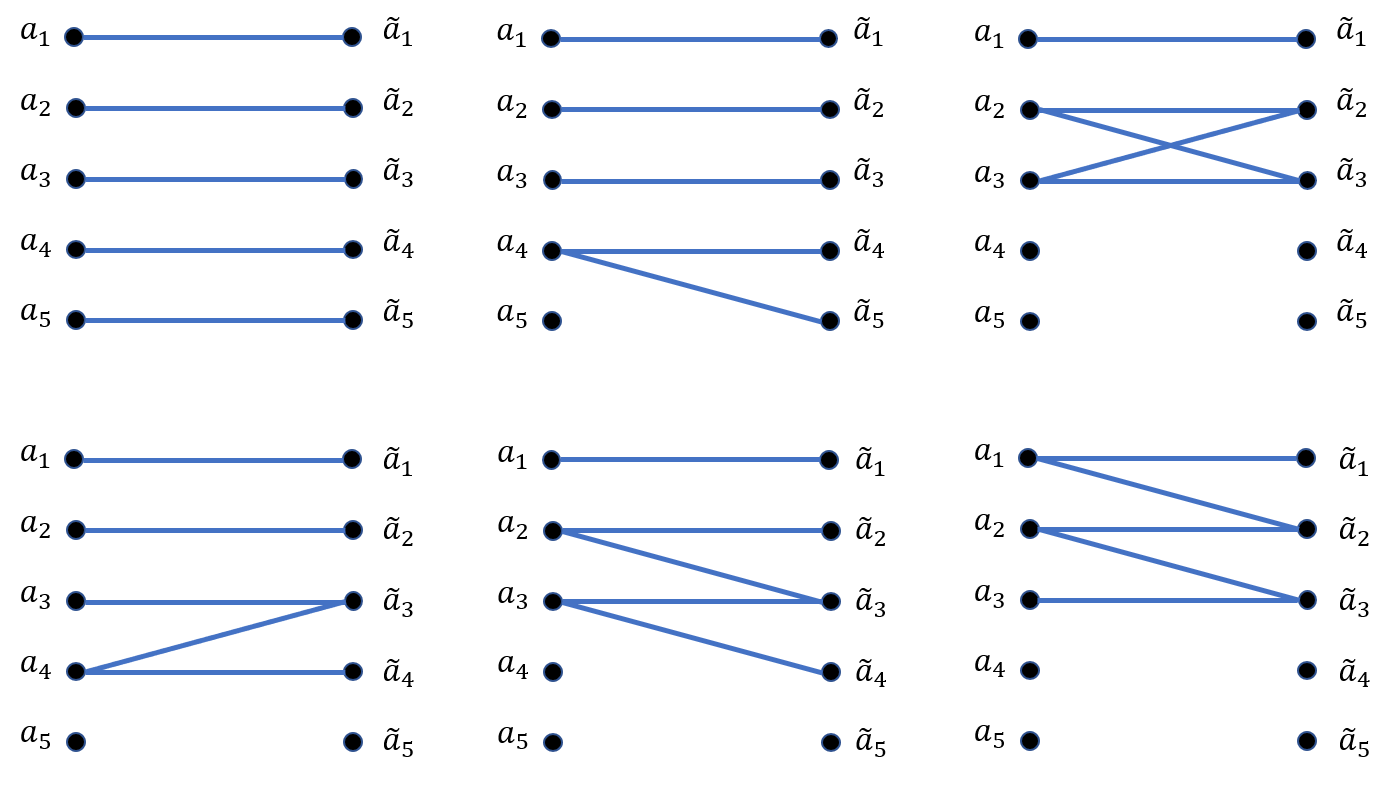
\includegraphics[width=\linewidth]{画像/辺5本の場合.png}
\vspace*{-1cm}
\caption{辺数が5である二分グラフの例(各頂点の次数は2以下)}
\label{辺5本の場合}
\end{figure}

図\ref{辺5本の場合}のように,ある$\tilde{G}_{i}$に含まれる辺が5本であるとき,互いに隣接しない辺が3本以上存在する.
よって,補題\ref{補題14}(abc)より,$p \{x:=xy \} \preceq q_{k}$となる.
これは,仮定に矛盾する.

\textbf{(2-2)} 
$p \{ x:=ya_{i} \} \preceq q_{i}$かつ$p \{ x:=a_{i}y \} \preceq q_{i}$ $(i=1, \ldots, k-3)$とし,$p \{ x:=ya_{j+3} \} \preceq q_{j}$かつ$p \{ x:=a_{j}y \} \preceq q_{j}$ $(j=k-2,k-1)$とする.
このとき,系\ref{両方}より,$p \{ x:=a_{j+3}a_{j} \} \preceq q_{j}$となる$q_{j}$が考えられる.
よって,$\tilde{G}_{j}$には,それぞれ1本の辺が含まれる.
$G$に含まれる辺は,9本であるから,残り$9-2=7$本の辺は$\tilde{G}_{i}$ $(i=1, \ldots, k-3)$と$\tilde{G}_{k}$に含まれる.
$\tilde{G}_{i}$のいずれかに,辺が1本以上含まれる場合,$p \{ x:=ab \} \preceq q_{i}$ $(a \not = a_{i}$かつ$b \not = a_{i})$となる.
補題\ref{追加部分}より,$p \{ x:=xy \} \preceq q_{i}$となる
これは,仮定に矛盾する.
よって,$\tilde{G}_{k}$には$7$本の辺が含まれる.
ある$\tilde{G}_{i}$に含まれる辺が5本以上であるとき,互いに隣接しない辺が3本以上存在する.
補題\ref{補題14}(abc)より,$p \{x:=xy \} \preceq q_{k}$となる.
これは,仮定に矛盾する.

\textbf{(2-3)} 
$p \{ x:=ya_{i} \} \preceq q_{i}$かつ$p \{ x:=a_{i}y \} \preceq q_{i}$ $(i=1, \ldots, k-2)$とし,$p \{ x:=ya_{k+2} \} \preceq q_{k-1}$かつ$p \{ x:=a_{k-1}y \} \preceq q_{k-1}$とする.
このとき,系\ref{両方}より,$p \{ x:=a_{k+2}a_{k-1} \} \preceq q_{k-1}$となる$q_{k-1}$が考えられる.
よって,$\tilde{G}_{k-1}$には,1本の辺が含まれる.
$G$に含まれる辺は,9本であるから,残り$9-1=8$本の辺は$\tilde{G}_{i}$ $(i=1, \ldots, k-2)$と$\tilde{G}_{k}$に含まれる.
$\tilde{G}_{i}$のいずれかに,辺が1本以上含まれる場合,$p \{ x:=ab \} \preceq q_{i}$ $(a \not = a_{i}$かつ$b \not = a_{i})$となる.
補題\ref{追加部分}より,$p \{ x:=xy \} \preceq q_{i}$となる.
これは,仮定に矛盾する.
よって,$\tilde{G}_{k}$には$8$本の辺が含まれる.
ある$\tilde{G}_{i}$に含まれる辺が5本以上であるとき,互いに隣接しない辺が3本以上存在する.
補題\ref{補題14}(abc)より,$p \{x:=xy \} \preceq q_{k}$となる.
これは,仮定に矛盾する.

\textbf{(2-4)} 
$p \{ x:=ya_{i} \} \preceq q_{i}$かつ$p \{ x:=a_{i}y \} \preceq q_{i}$ $(i=1, \ldots, k-1)$とする.
$\tilde{G}_{i}$のいずれかに,辺が1本以上含まれる場合,$p \{ x:=ab \} \preceq q_{i}$ $(a \not = a_{i}$かつ$b \not = a_{i})$となる.
補題\ref{追加部分}より,$p \{ x:=xy \} \preceq q_{i}$となる.
よって,$\tilde{G}_{k}$に$9$本の辺が含まれる.
ある$\tilde{G}_{i}$に含まれる辺が5本以上であるとき,互いに隣接しない辺が3本以上存在する.
補題\ref{補題14}(abc)より,$p \{x:=xy \} \preceq q_{k}$となる.
これは,仮定に矛盾する.

\noindent\textbf{(3)}
$G^{(k-2,k-2)}$には$4\times4=16$本の辺が含まれる.
$| A^{\prime} \cap B^{\prime} | = 0$であるとき,最大$4$つの$\tilde{G}_{i}$に辺が1本含まれ,$\tilde{G}^{(0,0)}_{i_{0}}$と$\tilde{G}^{(0,0)}_{i_{1}}$に,少なくとも$4 \times 4-4=12$本の辺が含まれる.
$12 > 4 \times 2 + 1$より,$\tilde{G}^{(0,0)}_{i_{0}}$または$\tilde{G}^{(0,0)}_{i_{1}}$は$5$本以上の辺を含む.
よって,$\tilde{G}^{(0,0)}_{i_{0}}$または$\tilde{G}^{(0,0)}_{i_{1}}$は,互いに隣接しない辺を3本以上含む.
したがって,補題\ref{補題14}(abc)より,$p \{x:=xy \} \preceq q_{i_{0}}$または$p \{x:=xy \} \preceq q_{i_{1}}$となる.
これは,仮定に矛盾する.  

$| A^{\prime} \cap B^{\prime} |=0$であるとき,$\tilde{G}^{(0,0)}_{i_{0}}$と$\tilde{G}^{(0,0)}_{i_{1}}$に含まれる辺数が最も少なくなる.
よって,$| A^{\prime} \cap B^{\prime} |=0$であるとき,矛盾であれば,$| A^{\prime} \cap B |=n$ $(n=1,2,3,4)$であるときも矛盾する.

一般化して考えていくと,$G$には$\sharp A^{\prime} \times \sharp\tilde{B}^{\prime}$本の辺が含まれる.
$| A^{\prime} \cap B^{\prime} |=0$であるとき,1本の辺を持つ$\tilde{G}^{(1,1)}_{i_{n}}$ $(n=1,\ldots, \ell$ $(0 \le \ell \le \sharp A^{\prime}))$が最大$\sharp A^{\prime}$個存在する.
このとき,$\tilde{G}^{(0,0)}_{j_{m}}$ $(m=1,\ldots, \sharp A^{\prime}-2)$には$\sharp A^{\prime} \times \sharp\tilde{B}^{\prime} - \ell$本の辺が含まれる.
よって,$\ell \le \sharp A^{\prime}$より,少なくとも$\sharp A^{\prime} \times \sharp\tilde{B}^{\prime} - \sharp A^{\prime}$本の辺が含まれる.
$\sharp A^{\prime}-2$個の$\tilde{G}^{(0,0)}_{j_{m}}$に対して,合計$4(\sharp A^{\prime}-2) +1$本の辺を追加していくと,少なくとも1個のグラフは,5本以上の辺を含む.
%\begin{equation*}\label{ine}
  %\begin{split}

\begin{center}
  \begin{tabular}{l}
  $\sharp A^{\prime} \times \sharp\tilde{B}^{\prime} -\sharp A^{\prime} \ge 4(\sharp A^{\prime}-2)+1$\\
  $\sharp A^{\prime 2}-\sharp A^{\prime} \ge 4\sharp A^{\prime}-8+1$\\
%  &\sharp A^{\prime 2}-\sharp A^{\prime}-4\sharp A^{\prime}+7 \ge 0\\
  $\sharp A^{\prime 2}-5\sharp A^{\prime}+7 \ge 0$~~~~~~~~~~~~~~~~~~~~~~~~~(1)
\end{tabular}
\end{center}
  %\end{split}
  %\end{equation*}


(1)式の判別式を$D$とすると,$D=25-4\times7=-3$となる.
$D<0$より,任意の$\sharp A^{\prime}$について不等式が成り立つ.
よって,ある$\tilde{G}^{(0,0)}_{i}$に含まれる辺は5本以上となり,互いに隣接しない辺が3本以上存在する.
したがって,補題\ref{補題14}(abc)より,$p \{x:=xy \} \preceq q_{i}$となる.
これは,仮定に矛盾する.  

以上より,$k \ge 2$においても,仮定に矛盾する.
\end{proof}

\begin{lem}[Sato et al.\cite{Sato1}]\label{補題15}
$\sharp \Sigma \ge 3$とし,$p,q$を正規パターンとする.
このとき,ある$a \in \Sigma$に対して,
$p \{ x := a \} \preceq q$かつ$p \{ x := xy \} \preceq q$ならば$p \preceq q$である.
ただし,$y$は$q$に含まれない変数記号である.
\end{lem}

補題\ref{追加補題1},補題\ref{補題15}より,次の定理が成り立つ.

\begin{thm}\label{定理17}
$k \ge 3$,$\sharp \Sigma \ge 2k-1$,$P \in \RPatplus,Q \in \RPat^{k}$とする.
このとき,以下の{\rm (i),(ii),(iii)}は同値である.
\[
\begin{tabular}{ll}
$(\mathrm{i})$ $S_{2}(P) \subseteq L(Q),$
$(\mathrm{ii})$ $P \sqsubseteq Q,$
$(\mathrm{iii})$ $L(P) \subseteq L(Q).$
\end{tabular}
\]
\end{thm}

\begin{proof}
(ii) $\Rightarrow$ (iii)と(iii) $\Rightarrow$ (i)は自明である.
定理\ref{定理10}より,$\sharp\Sigma \ge 2k+1$のとき,(i) $\Rightarrow$ (ii)は成り立つ.
よって,$\sharp Q=k$のとき,$\sharp\Sigma = 2k-1$または$\sharp\Sigma = 2k$の場合,(i) $\Rightarrow$ (ii)が成り立つことを,$p$に含まれる変数記号の数$n$に関する数学的帰納法により証明する.

$n=0$のとき,$S_{2}(p)= \{ p \}$であり,$p \in L(Q)$となる.よって,ある$q \in Q$に対して,$p \preceq q$となる.

$n \ge 0$個の変数記号を含む任意の正規パターンに対して題意が成り立つと仮定する.
$p$を$S_{2}(p) \subseteq L(Q)$を満たす$n+1$個の変数記号を含む正規パターンとする.
$p \not \preceq q_{i}$ ($i=1, \ldots, k$)と仮定する.
$p=p_{1}xp_{2}$ ($p_{1},p_{2}$は正規パターン,$x$は変数記号),$Q=\{ q_{1}, \ldots , q_{k} \}$を考える.
$a, b \in \Sigma$に対して,$p_{a}=p \{ x := a \}$と$p_{ab}=p \{ x := ab \}$とおく.
このとき,$p_{a},p_{ab}$は$n$個の変数記号が含まれ,$S_{2}(p_{a}) \subseteq L(Q)$かつ$S_{2}(p_{ab}) \subseteq L(Q)$が成り立つことに注意する.
帰納法の仮定より,任意の$a,b \in \Sigma$に対して,$p_{a} \preceq q_{i}$かつ$p_{ab} \preceq q_{i^{\prime}}$を満たすような$i, i^{\prime} \le k$が存在する. 
$D_{i}=\{ a \in \Sigma \mid p \{ x:=a \} \preceq q_{i} \}$ \ ($i=1, \ldots, k$)とする.
ある$i$に対して,$\sharp D_{i} \ge 3$であるとき,補題\ref{補題10}より,$p \preceq q_{i}$となる.これは仮定に矛盾する.
よって,$\sharp D_{i} \le 2$ ($i=1, \ldots, k$)となる場合を考える.
$\sharp\Sigma = 2k-1$のとき,任意の$i$に対して,$\sharp D_{i}=2$または$\sharp D_{i}=1$,$\sharp\Sigma = 2k$のとき,任意の$i$に対して,$\sharp D_{i}=2$となる.
$k \ge 3$であるとき,$2k+1 \ge k+2$となる.
よって,補題\ref{追加補題1}より,$p \{ x:=xy \} \preceq q_{i}$となる$i$が存在する.
したがって,補題\ref{補題15}より,$p \preceq q_{i}$となる.
これは仮定に矛盾する.
  
以上より,(i) $\Rightarrow$ (ii)が成り立つ.
\end{proof}

この定理\ref{定理17}より,次の系が得られる.

\begin{col}\label{命題18}
$k \ge 3$,$\sharp\Sigma \ge 2k-1$,$P \in \mathcal{RP}^{+}$とする.このとき,$S_{2}(P)$は$\mathcal{RPL}^{k}$における$L(P)$の特徴集合である.
\end{col}

\begin{lem}[Sato et al.\cite{Sato1}]\label{補題19}
$\sharp\Sigma \le 2k-2$とする.このとき,$\mathcal{RP}^{k}$は包含に関するコンパクト性を持たない.
\end{lem}

\begin{proof}
$\Sigma = \{ a_{1}, \ldots , a_{k-1}, b_{1}, \ldots , b_{k-1} \}$を$(2k-2)$個の定数記号から成る集合,$p, q_{i}$を正規パターン,$w_{i}~(i = 1, \ldots , k-1)$を例\ref{例題1}と同様に定義された記号列とする.
$q_{k} = x_{1}a_{1}w_{1}xyw_{1}b_{1}x_{2}$とする.
例\ref{例題1}で示した通り,$p \{ x := a_{i} \} \preceq q_{i}$かつ$p \{ x := b_{i} \} \preceq q_{i}~(i=1,2, \ldots ,k-1)$であるとき,$S_{1}(p) \subseteq \bigcup^{k-1}_{i=1} L(q_{i})$となる. 
一方で,任意の$w$ $(|w| \ge 2)$に対して,$p \{ x:= w \} \preceq q_{k}$となる. 
すなわち,$L(p) \subseteq L(Q)$である.
しかし,$p \not \preceq q_{i}$であるため,$L(p) \not \subseteq L(q_{i}) (i=1,2, \ldots k)$である.
したがって,$\RPatkei$は包含に関するコンパクト性を持たない.
\end{proof}

定理\ref{定理17}と補題\ref{補題19}より,次の定理が成り立つ.

\begin{thm}
$k \ge 3$とし,$\sharp\Sigma \ge 2k-1$とする.
このとき,$\RPat^{k}$は包含に関してコンパクト性を持つ.
\end{thm}

$k=2$のとき,次の定理が成り立つ.

\begin{thm}\label{補題21}
$\sharp \Sigma \ge 4$とし,$P \in \RPatplus$,$Q \in \RPat^{2}$とする.
このとき,以下の{\rm (i),(ii),(iii)}は同値である.
\[
\begin{tabular}{ll}
$(\mathrm{i})$ $S_{2}(P) \subseteq L(Q),$
$(\mathrm{ii})$ $P \sqsubseteq Q,$
$(\mathrm{iii})$ $L(P) \subseteq L(Q).$
\end{tabular}
\]
\end{thm}

\begin{proof}
(ii) $\Rightarrow$ (iii)と(iii) $\Rightarrow$ (i)は自明に成り立つ.
よって,(i) $\Rightarrow$ (ii)が成り立つことを示す.
$Q= \{ q_{1}, q_{2} \}$とするとき,$p$に含まれる変数記号の数$n$に関する数学的帰納法で示す.\\
\noindent (1) $n=0$のとき,$p$は定数記号列となるので$S_{2}(p)= \{ p \}$となり
(i)より,$p \in L(Q)$となる.
よって,ある$q \in Q$に対して$p \preceq q$となる.\\
\noindent (2) $n=k$個の変数記号を含むすべての正規パターンに対して有効であると仮定する.
そして,$p$を$S_{2}(p) \subseteq L(Q)$を満たす$(n+1)$個の変数記号を含む正規パターンとする.

$p \not \preceq q_{i}$ ($i=1, 2$)と仮定する.
$p=p_{1}xp_{2}$ ($p_{1}, p_{2}$は正規パターン,$x$は変数記号)を考える.
$a, b \in \Sigma$に対して,$p_{a}=p \{ x := a \}$,$p_{ab}=p \{ x := ab \}$とおく.
このとき,$p_{a},p_{ab}$は$n$個の変数記号が含まれ,$S_{2}(p_{a}) \subseteq L(Q)$,$S_{2}(p_{ab}) \subseteq L(Q)$が成り立つことに注意する.
帰納法の仮定より,任意の$a, b \in \Sigma$に対して,$p_{a} \preceq q_{i}, p_{ab} \preceq q_{i^{\prime}}$を満たすような$i, i^{\prime} \le k$が存在する.

ある$i$に対して$\sharp D_{i} \ge 3$のとき,補題\ref{補題10}より,$p \preceq q_{i}$となる.
よって,任意の$i$に対して,$\sharp D_{i} \le 2$となる.
したがって,$\sharp D_{1}=2$かつ$\sharp D_{2}=2$となる場合を考える.

$\sharp \Sigma = k+2$であるとき,$k=2$より,$\sharp \Sigma =4$となる.
よって,補題\ref{追加補題1}より,ある$i$に対して,$p \{ x:=xy \} \preceq q_{i}$となる.
したがって,補題\ref{補題15}より,$p \preceq q_{i}$となる.
これは,仮定に矛盾する.

以上より,(i) $\Rightarrow$ (ii)が成り立つ.
\end{proof}

次の例は,$k = 2$における定理\ref{補題21}の反例である.
\begin{ex}\label{反例thm17}
$\Sigma= \{a, b, c \}$を$3$つの定数記号から成る集合,$p,q_{1},q_{2}$を正規パターン,$x,x^{\prime},x^{\prime\prime}$を変数記号とする.
\begin{eqnarray*}
p = x^{\prime}axbx^{\prime\prime},
q_{1} = x^{\prime}abx^{\prime\prime},
q_{2} = x^{\prime}cx^{\prime\prime}.
\end{eqnarray*}
$w \in \Sigma^{+}$とする.$w$に$c$が含まれるとき,$p \{ x:=w \} \preceq q_{2}$となり,$c$が含まれないとき,$p \{ x:=w \} \preceq q_{1}$となる.
よって,$L(p) \subseteq L(q_{1}) \cup L(q_{2})$である.
しかし,$p \not \preceq q_{1}$かつ$p \not \preceq q_{2}$である.
\end{ex}

定理\ref{補題21}より,次の2つの系が成り立つ.
\begin{col}
$\sharp\Sigma \ge 4$とし,$P \in \RPatplus$とする.
このとき,$S_{2}(P)$は,$\RPatL^{2}$における$L(P)$の特徴集合である.
\end{col}

\begin{col}
$\sharp\Sigma \ge 4$とする.このとき,クラス$\mathcal{RP}^{2}$は包含に関してコンパクト性を持つ.
\end{col}



\section{非隣接変数正規パターン}

隣接した変数記号を持たない正規パターンを\textbf{非隣接変数正規パターン}という.
例えば,パターン$axybc$は正規パターンであるが,非隣接変数正規パターンではない.パターン$axbcy$は非隣接変数正規パターンである.
$\NAVRP$を非隣接変数正規パターン全体の集合とする.
$\NAVRP$の空でない有限部分集合の集合を$\NAVRPplus$で,
高々$k~(k\geq 1)$個のパターンから成る$\NAVRP$の部分集合$\{P\in \NAVRPplus \mid \sharp P \leq k\}$を$\NAVRPkei$で表す.
このとき,次の定理が成り立つ.

\begin{thm}\label{非隣接kが4以上}
$\sharp \Sigma \ge k+2,P\in \NAVRPplus,Q \in \NAVRPkei$とする.
このとき,以下の{\rm (i), (ii), (iii)}は同値である.
\[
\begin{tabular}{ll}
$(\mathrm{i})$ $S_{2}(P) \subseteq L(Q),$
$(\mathrm{ii})$ $P \sqsubseteq Q,$
$(\mathrm{iii})$ $L(P) \subseteq L(Q).$
\end{tabular}
\]
\end{thm}

\begin{proof}
定義より,
(ii) $\Rightarrow$ (iii)と(iii) $\Rightarrow$ (i)は自明に成り立つ.
よって,(i) $\Rightarrow$ (ii)が成り立つことを,$p$に現れる変数記号の数$n$に関する数学的帰納法で証明する.

$n=0$のとき,$S_{2}(p)= \{ p \}$であり,$p \in L(Q)$となる.よって,ある$q \in Q$に対して,$p \preceq q$となる.

$n \ge 0$個の変数記号を含む任意の正規パターンに対して,題意が成り立つと仮定する.
$p$を$S_{2}(p) \subseteq L(Q)$を満たす$n+1$個の変数記号を含む非隣接変数正規パターンとする.
$p \not \preceq q_{i}$ ($i=1, 2$)と仮定する.
非隣接変数正規パターン$p$を$p=p_{1}xp_{2}$, $Q=\{ q_{1}, \ldots , q_{k} \}$とおく.
ここで,$p_{1}$は末尾が定数記号である非隣接変数正規パターンであり,$p_{2}$は先頭が定数記号である非隣接変数正規パターン,$x$は変数記号,任意の$i$ ($i=1, \ldots, k$)に対して,$q_{i}$は非隣接変数正規パターンである.
$a, b \in \Sigma$に対して,$p_{a}=p \{ x := a \}$,$p_{ab}=p \{ x := ab \}$とおく.
このとき,$p_{a}, p_{ab}$は$n$個の変数記号が含まれ,$S_{2}(p_{a}) \subseteq L(Q)$かつ$S_{2}(p_{ab}) \subseteq L(Q)$が成り立つことに注意する.
帰納法の仮定より,任意の$a, b \in \Sigma$に対して,$p_{a} \preceq q_{i}$かつ$p_{ab} \preceq q_{i^{\prime}}$を満たすような$i, i^{\prime} \le k$が存在する.

補題\ref{追加補題1}より,ある$i$に対して$p \{ x:=xy \} \preceq q_{i}$が成り立つ.
このとき,$p \{ x:=xy \} =p_{1}xyp_{2}$の部分パターン$xy$は$q_{i}$の変数記号を置き換えることで生成できない.
このことは,$q_{i}$に$xy$が含まれることを示している.
これは,$q_{i}$が非隣接変数正規パターンであることに矛盾する.

以上より,(i) $\Rightarrow$ (ii)が成り立つ.
\end{proof}

\begin{col}
$\sharp\Sigma \ge k+2$,$P \in \NAVRPplus$とする.このとき,$S_{2}(P)$は$\mathcal{RPL^{\mbox{$k$}}_{NAV}}$における$L(P)$の特徴集合である.
\end{col}

\begin{lem}\label{k+2のとき}
$\sharp\Sigma \le k+1$とする.このとき,$\NAVRPkei$は包含に関してコンパクト性を持たない.
\end{lem}
\begin{proof}
$\Sigma = \{ a_{1}, \ldots , a_{k+1} \}$を$k+1$個の定数記号から成る集合,$p, q_{i}$を正規パターンとする.
$p \{ x := a_{i}y \} \preceq q_{i}$かつ$p \{ x := ya_{i+1} \} \preceq q_{i}~(i=1,2, \ldots ,k)$とする.
$p \{ x:= a_{k+1}a_{1} \} \preceq q_{1}$であるとき,$S_{2}(p) \backslash S_{1}(p) \subseteq \bigcup^{k}_{i=1} L(q_{i})$となる. 
すなわち,$L(p) \subseteq L(Q)$である.
しかし,$p \not \preceq q_{i}$であるため,$L(p) \not \subseteq L(q_{i})~(i=1,2, \ldots k)$である.
したがって,$\NAVRPkei$は包含に関するコンパクト性を持たない.
\end{proof}

コンパクト性をもたない例を例\ref{反例k+1}に示す.
\begin{figure*}[tb]
\begin{ex}\label{反例k+1}
$\Sigma= \{a_{1}, a_{2}, a_{3},a_{4} \}$を$4$つの定数記号から成る集合,$p,q_{1},q_{2},q_{3}$を正規パターン,$x,x^{\prime},x^{\prime\prime}$を変数記号とする.
$p,q_{1},q_{2},q_{3}$を以下のように定義する.
\begin{align*}
p & = x^{\prime}a_{3}a_{1}a_{4}a_{1}a_{4}a_{1}a_{1}a_{4}a_{1}a_{3}a_{2}a_{1}a_{4}a_{1}a_{4}a_{1}a_{1}a_{4}a_{1}xa_{1}a_{4}a_{1}a_{4}a_{1}a_{1}a_{4}a_{1}a_{3}a_{2}a_{1}a_{4}a_{1}a_{4}a_{1}a_{1}a_{4}a_{1}a_{2}x^{\prime\prime},\\
q_{1} & = x^{\prime}a_{3}a_{1}a_{4}a_{1}a_{4}a_{1}a_{1}a_{4}a_{1}a_{3}a_{2}a_{1}a_{4}a_{1}a_{4}a_{1}a_{1}a_{4}a_{1}a_{2}x^{\prime\prime},\\
q_{2} & = x^{\prime}a_{2}a_{1}a_{4}a_{1}a_{4}a_{1}a_{1}a_{4}a_{1}a_{3}x^{\prime\prime},\\
q_{3} & = x^{\prime}a_{1}a_{1}a_{4}a_{1}a_{4}x^{\prime\prime}.
\end{align*}

これは,$L(p) \subseteq L(q_{1}) \cup L(q_{2}) \cup L(q_{3})$となる.
しかし,$p \not \preceq q_{1},p \not \preceq q_{2}$かつ$p \not \preceq q_{3}$である.
\end{ex}
\end{figure*}

定理\ref{非隣接kが4以上}と補題\ref{k+2のとき}より,次の定理が成り立つ.

\begin{thm}
$\sharp\Sigma \ge k+2$とする.
このとき,$\RPat^{k}$は包含に関してコンパクト性を持つ.
\end{thm}

\section{おわりに}
本稿では,高々$k$ $(k\ge 2)$個の正規パターン集合全体のクラス$\RPatkei$について,(1) 正規パターン集合$P\in\RPatkei$から得られる記号列の集合$S_2(P)$が$P$により生成される言語$L(P)$の特徴集合となること,
および(2) $\RPatkei$が包含に関してコンパクト性を持つこと
を示したSatoら\cite{Sato1}の結果の証明の誤りを修正した.
次に,隣接する変数がない正規パターンである非隣接変数正規パターンについて,
高々$k(k\ge 3)$個の非隣接変数正規パターン集合全体のクラス$\NAVRPkei$から得られる記号列の集合$S_2(P)$が,
正規パターン言語の有限和に対する特徴集合と,定数記号の数が$k+2$以上のとき,
$\NAVRPkei$が包含に関してコンパクト性をもつことを示した.
これらにより,Arimuraら\cite{Arimura1994}が示した$\RPatkei$に対する学習アルゴリズムを非隣接変数正規パターン言語の有限和に関する効率的な学習アルゴリズムが設計できることを示した.

今後の課題として,$\NAVRPkei$に対する特徴集合を活用し,非隣接変数正規パターン言語の有限和を正例から極限同定する多項式時間帰納推論アルゴリズム
および一つの正例と多項式回の所属性質問を用いて同定する質問学習アルゴリズムの高速化が考えられる.
また,正規パターン言語の有限和に対する特徴集合の概念を
線形項木パターン言語\cite{Suzuki2006}の有限和や正則FGS言語\cite{Uchida1994}に拡張することが考えられる.



\section*{謝辞}
本研究はJSPS科研費 19K12103, 20K04973, 21K12021, 22K12172の助成を受けたものである.

\input{LA-summer.bib}

\end{document}
